\documentclass[11pt]{article}
\usepackage[margin=0.85in]{geometry}
\usepackage[T1]{fontenc}
\usepackage{lmodern}
\usepackage{microtype}
\usepackage{amsmath,amssymb,mathtools}
\usepackage{booktabs,longtable,array,tabularx}
\usepackage{xcolor}
\usepackage{tikz}
\usetikzlibrary{arrows.meta,positioning,calc}
\definecolor{pfnblue}{RGB}{36,76,117}
\definecolor{pfngreen}{RGB}{41,103,86}
\definecolor{pfnamber}{RGB}{145,93,30}
\tikzset{
 pfnbox/.style={draw=pfnblue!75,fill=pfnblue!4,rounded corners=2pt,
   align=center,inner sep=6pt,font=\small,minimum height=13mm},
 pfndata/.style={pfnbox,draw=pfngreen!80,fill=pfngreen!5},
 pfnhidden/.style={pfnbox,draw=pfnamber!85,fill=pfnamber!5,dashed},
 pfnarrow/.style={-{Latex[length=2.2mm]},thick,draw=pfnblue!85},
 pfnloss/.style={-{Latex[length=2.2mm]},thick,dashed,draw=pfnamber!90}
}
\usepackage{enumitem}
\usepackage{needspace}
\usepackage{hyperref}
\usepackage{fancyhdr}
\usepackage{listings}
\hypersetup{colorlinks=true,linkcolor=blue!45!black,urlcolor=blue!55!black,citecolor=blue!45!black,pdftitle={Tabular In-Context Learning: Priors, Architecture, and Training}}
\setlength{\parskip}{5pt}
\setlength{\parindent}{0pt}
\setlist{nosep,leftmargin=*}
\setlength{\emergencystretch}{2em}
\renewcommand{\arraystretch}{1.16}
\newcolumntype{Y}{>{\raggedright\arraybackslash}X}
\newcommand{\E}{\mathbb{E}}
\newcommand{\R}{\mathbb{R}}
\newcommand{\ind}{\mathbf{1}}
\newcommand{\given}{\,\vert\,}
\newcommand{\evidence}{\textbf{Evidence.} }
\newcommand{\proposal}{\textbf{Proposal.} }
\newcommand{\risk}{\textbf{Failure mode.} }
\pagestyle{fancy}
\fancyhf{}
\fancyhead[L]{\small Tabular in-context learning: recipe and evidence}
\fancyhead[R]{\small Research assessment / 3 October 2026}
\fancyfoot[C]{\thepage}
\setlength{\headheight}{14pt}
\lstset{basicstyle=\ttfamily\small,breaklines=true,columns=fullflexible,frame=single,rulecolor=\color{black!20}}
\title{Tabular In-Context Learning:\protect\\Priors, Architecture, and Training\protect\\[6pt]\large A research proposal for standard benchmarks and rare-event prediction}
\author{Research assessment prepared for Niraj Kumar}
\date{3 October 2026}
\begin{document}
\maketitle
\thispagestyle{empty}

\begin{abstract}
\noindent Prior-fitted tabular models learn a prediction procedure from synthetic tasks and apply it to new tables through in-context learning. Their performance depends jointly on the training distribution, the representation of features and targets, and the use of labeled context. This report develops a pretraining proposal for binary classification, multiclass classification and regression, with an additional emphasis on large financial tables containing missing values and fraud rates near $10^{-4}$.

The proposed model uses a dense 317M-parameter backbone, categorical hash-bit inputs, a quantile regression head and shared query KV heads. Its executable reference pilot combines the released TabICLv2 graph generator with a small hierarchical-category extension. We propose a broader challenger that allocates 50/20/15/10/5 percent of requested tasks to graph, direct-forest, hierarchical-category, smooth/local and sparse-interaction mechanisms, each subject to an explicit observation law. The challenger sampler and a compact persistent-cell comparator are implemented. Staged comparisons will select the weights and architecture. A separate fraud continuation uses finite populations with delayed labels and the context-selection policy intended for deployment.

The proposal draws on recent tabular foundation models and analyses of finite-context information, loss estimation and representation precision. It specifies the generators, architecture, optimization, curriculum and evaluation within a 50,000 GPU-hour budget. Local tests verify implementation properties and reproduce diagnostic counterexamples. Benchmark accuracy, optimal training scale and GPU latency remain to be established.
\end{abstract}

\begin{center}
\fbox{\begin{minipage}{0.93\linewidth}
\textbf{Research and training sequence.} Select the standard prior using the costed comparisons in Section~\ref{sec:prior-selection}, then train the chosen prior--architecture pair and retain a separate fraud specialist. The existing 64M standard-task and 1.024M finance-task targets are provisional ceilings for planning, not evidence selecting the R/P1 pilot as the final bank.
\end{minipage}}
\end{center}
\clearpage
{\small\setlength{\parskip}{0pt}\tableofcontents}
\clearpage

\section{Problem setting and research strategy}
\label{sec:decision}

A tabular in-context learner uses the labeled rows of a new table as evidence for predicting its unlabeled rows. Its parameters stay fixed during this process. The reusable object learned in pretraining is therefore a prediction procedure: it must recognize which relationships are supported by the available examples and use them on the query rows. We consider binary classification, multiclass classification and regression, and evaluate each separately whether the tasks share a checkpoint or use task-specific models. Context retrieval and permutation ensembles are explicit inference variants. Per-dataset gradient fine-tuning provides a separate adaptation baseline.

Two settings motivate the design. Standard tabular benchmarks test whether the learned procedure transfers across heterogeneous numerical and categorical tables. Financial prediction adds a different constraint: a table can contain millions of records while offering little evidence about a rare outcome. Missing features, delayed labels and bursts of arriving records further determine what can be used at prediction time. Both settings use the same table interface, but they place different demands on the prior and the way context is assembled.

The proposed training sequence retains a general tabular checkpoint and initializes a second checkpoint for binary fraud detection. An 80\% standard and 20\% finance mixture is retained as a comparison for parameter sharing. A \emph{macroepisode} denotes one supervised prediction task from a sampled world; in finance, its queries may be divided among several selected contexts.


The design links the generated task to the evidence the predictor can use. The prior determines which relationships occur and whether the available context can identify them. Numerical and category encoding, followed by row compression, determine how much of that evidence reaches the transformer. Optimization determines how the model spends its finite capacity and compute. These choices must therefore be studied together. The 317M model combines a broad reference prior with category occupancy, finer target representation and context selection matched to deployment. Comparisons with the unchanged reference and smaller architectures will test whether the additions justify their cost.

The report follows the same progression. Section~\ref{sec:prior-philosophy} explains how a distribution of synthetic tasks can teach inference from context. The literature review and analysis then motivate the generator and model specifications. Sections~\ref{sec:compute} and~\ref{sec:evaluation} give the compute allocation and empirical comparison; Section~\ref{sec:experiments} maps the method to executable code and records the completed checks.

The executable reference pilot and the implemented selection experiment are distinguished throughout. Section~\ref{sec:prior-selection} gives the current recommendation for choosing a stronger bank; earlier R/P1 volumes describe the runnable pilot, not a scientifically selected winner. A \emph{control} is a specified comparison, such as the original authored prior or coarse regression head. An \emph{extension} is a separate experiment whose implementation status is stated where it is introduced. Their full parameters are retained so that the comparisons are reproducible, but they are not additional components to turn on in the main run.

\subsection{Executable model and reference pilot}
\label{sec:main-candidate}

The model first represents individual cells, then forms row representations that can interact through labeled context. Two cell-encoding stages feed a 24-layer, width-1,024 row transformer. Categorical inputs use \texttt{hash\_bits}, ordinary regression uses 999 quantiles, and logarithmic length scaling adjusts attention with context size. The query path shares two KV heads, while support processing retains full-head attention. Section~\ref{sec:architecture-terms} explains these three architectural choices before their detailed specifications.

The compressed model has \textbf{317,116,304 parameters}. The implemented \texttt{persistent\_small} comparator has \textbf{41,089,248}; its geometry is specified in Section~\ref{sec:persistent-comparator}. This count includes an optional realized-loss head with a zero atom and a 1,025-bin positive density, reserved for a separate finance-regression experiment. The 94M model and released compact architectures provide lower-cost comparisons. Section~\ref{sec:compute} describes the experiments that will determine whether the additional capacity is useful.

For the executable standard pilot, the starting distribution is the released TabICLv2 graph generator, denoted R. Hierarchical category tasks, denoted P1, add repeated identities and shared effects that can be studied through category occupancy. The sampler fixes the task and table shape before choosing P1 with probability .05 when the requested width is at least eight; the remaining draws use R. Classification and regression each receive half the task mass in expectation.

R keeps its native filters. P1 uses validity checks without teacher filtering, keeping the acceptance law explicit for each source. In stages two and three, 20\% of requests use expanded feature and class limits. Together with the new model representation, these choices define an extension of the released system.

The finance model begins with the standard checkpoint and continues training on finite fraud populations. The original checkpoint is retained for general tabular prediction. During continuation, context selection and query weighting follow Section~\ref{sec:finance}, so the specialist learns from the same kinds of historical evidence it will receive at deployment. Its weights remain fixed when applied to a customer dataset. Final training reserves 9,000 GPU-hours for the standard model and 3,000 for the binary specialist. The architecture and generators also support finance regression, which requires an evaluation separate from the initial binary specialization.

The optimizer follows the parameter partition in Section~\ref{sec:optimizer}: Muon updates hidden matrices and AdamW updates the remaining parameters. Weight decay is zero in the candidate, following the released TabICLv2 script, and .01 in the authored control. Auxiliary, contrastive and adaptive-mixture losses are disabled in the main run, so the initial comparison concerns the prior and representation under supervised prediction losses.

The supplied \path{configs/candidate_standard.json} and \path{configs/candidate_fraud.json} configurations are bounded pilots. Section~\ref{sec:volume} specifies the proposed full task volumes and their throughput requirements; \path{docs/main_recipe.md} gives the run procedure.

\subsection{Categorical inputs, regression outputs and query attention}
\label{sec:architecture-terms}

The three terms describe different parts of the predictor. Categorical hash bits specify how a category enters the network. The quantile head specifies what the network predicts for a numerical target. Shared query KV heads specify how an unlabeled row reads information from labeled support.

\paragraph{Categorical hash-bit inputs.}
A categorical value identifies a group, such as a merchant or product, without defining a numerical order. Assigning merchant IDs 1, 2 and 3 does not make the third merchant three times the first. The encoder therefore gives each category a deterministic bit pattern. For a fixed feature namespace and recoding seed, the same category receives the same pattern in support and query.

The implementation takes 64 bits from a SHA-256 hash of the typed category key, feature identity and seed, then represents each bit by $-1$ or $+1$. For illustration, the four-bit pattern \texttt{1010} would become $(+1,-1,+1,-1)$; the actual representation has 64 coordinates. It appends support frequency, an unseen-category flag and a missing-value flag, giving 67 input coordinates. A learned linear projection converts these coordinates into the cell representation used by the transformer. Thus the hash is fixed, while the network learns how to use its output.

This representation accommodates categories absent from pretraining without allocating a separate learned lookup entry to every possible ID. It also keeps each raw identity bit exactly representable in BF16, unlike nearby scalar codes that can become indistinguishable after rounding. The bit pattern itself carries no merchant semantics or target risk: those relationships must be inferred from the other features and labeled context. Hash collisions and information loss after the learned projection remain possible. Section~\ref{sec:codec} specifies the support-only collision checks, missing-category encoding and precision tests.

\paragraph{A quantile regression head.}
A prediction head is the final learned mapping from a query's hidden representation to its outputs. For classification, those outputs determine class probabilities. For regression, the selected head predicts conditional percentiles of the numerical target, given the query features and labeled support. The 0.5 quantile is a median; the 0.9 quantile is an upper percentile intended to place approximately 90\% of conditional outcomes at or below it, with the usual qualification for discrete distributions.

For example, predicted 0.1, 0.5 and 0.9 quantiles of 20, 35 and 80 describe a median prediction of 35 and an intended central 80\% prediction interval from 20 to 80. This is an interval for an individual outcome, not a confidence interval for a fitted mean. Its actual coverage must be checked on held-out data. The model predicts 999 such values, at levels $\tau_k=k/1000$ for $k=1,\ldots,999$, through one shared network.

Each output is trained with the asymmetric absolute-error loss called the \emph{pinball loss}. If $e=z-\widehat q_\tau$ is the difference between the support-standardized target and its predicted quantile, then
\[
 \rho_\tau(e)=
 \begin{cases}
  \tau e,& e\geq0,\\
  (\tau-1)e,& e<0.
 \end{cases}
\]
At $\tau=0.9$, an underestimate has nine times the penalty of an equally large overestimate. This asymmetry makes the population loss favor the requested percentile. Training averages the 999 losses on the raw outputs. Prediction transforms them back to the target's original units and sorts them to give an ordered quantile curve. The point prediction averages the grid, approximating a conditional mean; it is distinct from taking the median. A finite grid does not specify a complete density or resolve arbitrarily rare tails. Section~\ref{sec:heads} gives the head specification, its comparison with histogram outputs and a rare-tail counterexample.

\paragraph{Shared query key/value heads.}
Attention uses learned \emph{query} (Q), \emph{key} (K) and \emph{value} (V) vectors. In the row transformer's prediction path, an unlabeled row supplies Q, and labeled support rows supply K and V. Comparing Q with each K determines attention weights; the weighted combination of V supplies information from support. An attention head performs this operation in one learned subspace. Different query heads can assign different weights to the same support rows.

The candidate retains 16 query heads but shares two sets of support K/V vectors among them. The first eight query heads use the first K/V head, and the remaining eight use the second. Their Q vectors are still distinct, so sharing K/V does not force their attention weights or outputs to be identical. The implementation first computes support self-attention with all 16 heads, then keeps the first two K/V heads in the cache used for queries. This is query-only grouped attention, applied consistently during training and inference.

At fixed support size and head dimension, retaining two K/V heads instead of sixteen makes the persistent trunk K/V cache eight times smaller. It does not remove support rows, reduce the number of query heads, or make the complete model eight times faster. Support preparation still uses full-head attention, other caches and activations remain, and backend kernels determine the realized bandwidth benefit. It also changes the predictor relative to independent K/V heads, so predictive quality requires comparison. Section~\ref{sec:latency-moe} gives the exact cache sizes and latency protocol.

\Needspace{4\baselineskip}
These mechanisms are implemented in \path{codec.py}, \path{model.py} and \path{distributions.py}: the codec constructs category identities, the model projects inputs and produces quantiles and attention states, and the loss module evaluates pinball scores. Section~\ref{sec:code-map} locates these modules in the repository.

\subsection{Scope of the empirical claims}

The mathematical arguments describe particular estimators, representations and attention patterns. To assess predictive performance, we need trained checkpoints compared with current methods on the same splits and within declared inference budgets. Binary classification, multiclass classification, regression and financial detection must therefore be reported separately, with uncertainty, failure coverage and latency.

A component is first compared on a matched backbone, then confirmed with independent seeds and dataset lineages. The complete configuration is subsequently tested across model sizes and training horizons. This sequence addresses two sources of uncertainty: a component can behave differently at larger scale, and improvements measured separately may fail to combine. The final comparison evaluates the resulting system rather than attributing its entire gain to any one component.



\section{How a prior teaches in-context prediction}
\label{sec:prior-philosophy}

In prior-based pretraining, we choose a distribution of prediction problems before training the network. A draw specifies relationships among columns, the target mechanism, noise and the observation process. It then produces a table on which the network must predict withheld outcomes from labeled examples. Repeating this process teaches the network how evidence in a new context should affect its predictions.

For example, the target may depend almost linearly on one feature, change sharply at a threshold, or share an effect across records with the same product code. Support observations help distinguish these explanations. The prior controls how often the learner encounters each possibility, including ambiguous cases in which several explanations fit the observed rows. This is why the bank is more than a source of training volume: it defines the inference problems that pretraining can teach.

\subsection{Prior, world, table and episode}

\begin{table}[ht]
\centering\small
\begin{tabularx}{\linewidth}{@{}p{.15\linewidth}Y@{}}
\toprule Object & Meaning in this project\\
\midrule
Prior family & A distribution over possible rules and data sets, such as R or P1. A family is a generator, not one stored table.\\
World $\phi$ & One sampled set of hidden rules: graph/functions, category effects, noise parameters, or a finite finance population.\\
Table & Records produced under a world. Their features and outcomes obey the same sampled mechanism, subject to its declared observation law.\\
Episode & A prediction exercise: labeled support, query features, and separate query targets used to score the prediction. A finance macroepisode may use several routed support contexts.\\
Neural weights $\theta$ & The shared predictor learned across many episodes. These are different from the hidden parameters $\phi$ of a particular synthetic world.\\
\bottomrule
\end{tabularx}
\caption{Generating 64 million tasks counts accepted episodes, not 64 million prior families, independent rows or parameters.}
\end{table}

A world is sampled before its records. For the rule $y=ax+\epsilon$, the coefficient $a$ stays fixed while new $x$ values and noise are drawn for each row. Another world can use a different $a$. If an unrelated slope were drawn for every record, support labels would generally cease to reveal a relationship that transfers to the query. The same principle applies to P1: an entity's latent effect is shared across its support and query occurrences. In finance, four macroepisodes reuse one finite population, giving four uses of the same world rather than four independent populations.

Sharing a world does not imply independent rows. Finite populations, time effects and sampling without replacement can introduce dependence. The native R source also transforms complete tables and applies acceptance tests. These operations change the prediction problem seen during training and are included in the prior specification.

\begin{figure}[htbp]
\centering
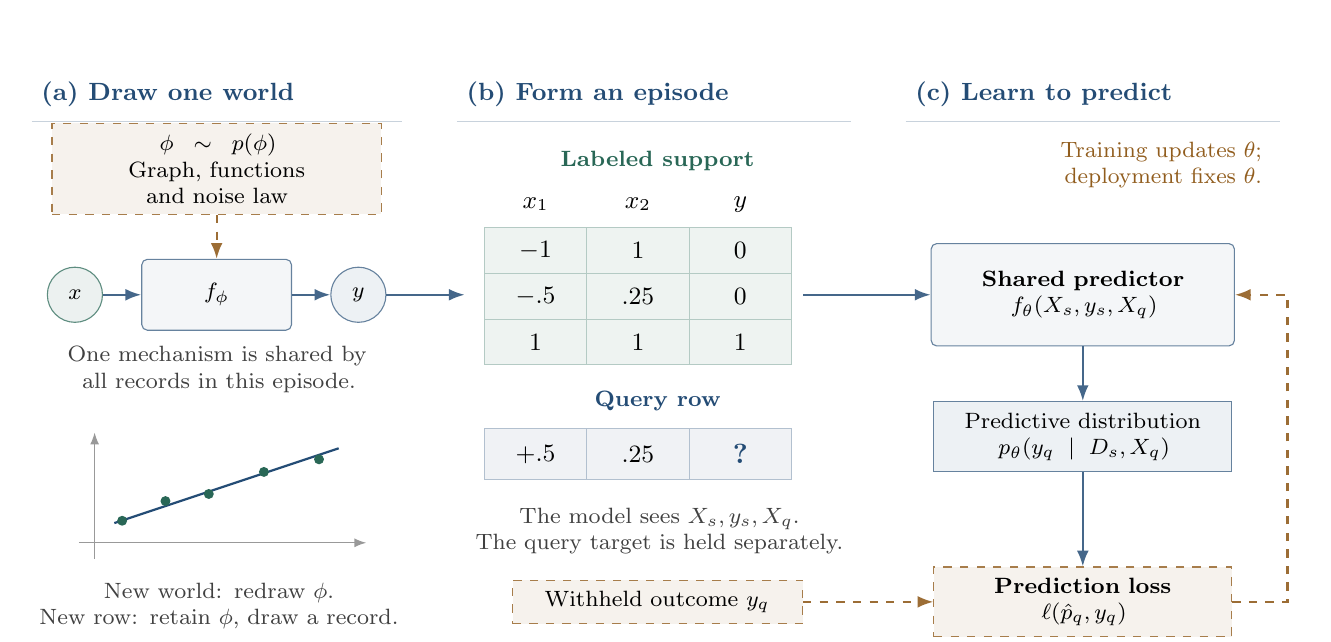
\begin{tikzpicture}[x=1cm,y=1cm,
  font=\small,
  panel/.style={draw=pfnblue!20,line width=.5pt,rounded corners=2pt,fill=white},
  title/.style={font=\small\bfseries,text=pfnblue,anchor=west},
  note/.style={font=\footnotesize,align=center,text=black!75},
  process/.style={font=\footnotesize,draw=pfnblue!70,fill=pfnblue!5,rounded corners=2pt,align=center,inner sep=5pt},
  support/.style={font=\footnotesize,draw=pfngreen!75,fill=pfngreen!9,align=center,inner sep=4pt},
  query/.style={font=\footnotesize,draw=pfnblue!70,fill=pfnblue!8,align=center,inner sep=4pt},
  hidden/.style={font=\footnotesize,draw=pfnamber!80,fill=pfnamber!8,align=center,inner sep=4pt,dashed},
  flow/.style={-{Latex[length=2mm]},draw=pfnblue!85,line width=.8pt},
  target/.style={-{Latex[length=2mm]},draw=pfnamber!90,line width=.8pt,dashed},
  reuse/.style={-{Latex[length=2mm]},draw=pfngreen!90,line width=.8pt,dashed}]

\path[use as bounding box] (0,.2) rectangle (16.2,-7.25);
\node[title] at (.05,-.15) {(a) Draw one world};
\node[title] at (5.45,-.15) {(b) Form an episode};
\node[title] at (11.15,-.15) {(c) Learn to predict};
\draw[pfnblue!25] (.05,-.5)--(4.75,-.5);
\draw[pfnblue!25] (5.45,-.5)--(10.45,-.5);
\draw[pfnblue!25] (11.15,-.5)--(15.9,-.5);
\node[hidden,text width=3.9cm] (phi) at (2.4,-1.1)
  {$\phi\sim p(\phi)$\\Graph, functions and noise law};
\node[support,circle,minimum size=7mm] (x) at (.6,-2.7) {$x$};
\node[process,text width=1.55cm,minimum height=9mm] (fun) at (2.4,-2.7) {$f_\phi$};
\node[query,circle,minimum size=7mm] (y) at (4.2,-2.7) {$y$};
\draw[flow] (x)--(fun);
\draw[flow] (fun)--(y);
\draw[target] (phi)--(fun);
\node[note,text width=4.5cm] at (2.4,-3.65)
  {One mechanism is shared by all records in this episode.};
\draw[-{Latex[length=1.5mm]},black!40] (.65,-5.85)--(4.3,-5.85);
\draw[-{Latex[length=1.5mm]},black!40] (.85,-6.05)--(.85,-4.45);
\draw[pfnblue,line width=.8pt] (1.1,-5.6)--(3.95,-4.65);
\foreach \xx/\yy in {1.2/-5.57,1.75/-5.32,2.3/-5.23,3/-4.95,3.7/-4.79}
  \fill[pfngreen] (\xx,\yy) circle (1.8pt);
\node[note,text width=4.5cm] at (2.4,-6.65)
  {New world: redraw $\phi$.\\New row: retain $\phi$, draw a record.};
\draw[flow] (4.55,-2.7)--(5.55,-2.7);
\node[font=\footnotesize\bfseries,text=pfngreen] at (8,-1) {Labeled support};
\foreach \xx/\lab in {6.45/$x_1$,7.75/$x_2$,9.05/$y$}
  \node at (\xx,-1.55) {\lab};
\foreach \rr in {0,1,2}{
  \foreach \cc in {0,1,2}{
    \draw[draw=pfngreen!35,fill=pfngreen!8] (5.8+1.3*\cc,-1.85-.58*\rr)
      rectangle ++(1.3,-.58);
  }
}
\foreach \xx/\yy/\val in {6.45/-2.14/-1,7.75/-2.14/1,9.05/-2.14/0,6.45/-2.72/-.5,7.75/-2.72/.25,9.05/-2.72/0,6.45/-3.30/1,7.75/-3.30/1,9.05/-3.30/1}
  \node at (\xx,\yy) {$\val$};
\node[font=\footnotesize\bfseries,text=pfnblue] at (8,-4.05) {Query row};
\foreach \cc in {0,1,2}
  \draw[draw=pfnblue!35,fill=pfnblue!7] (5.8+1.3*\cc,-4.4) rectangle ++(1.3,-.65);
\node at (6.45,-4.725) {$+.5$};
\node at (7.75,-4.725) {$ .25$};
\node[text=pfnblue,font=\bfseries] at (9.05,-4.725) {?};
\node[note,text width=4.6cm] at (8,-5.7)
  {The model sees $X_s,y_s,X_q$.\\The query target is held separately.};
\node[hidden,text width=3.4cm] (truth) at (8,-6.6) {Withheld outcome $y_q$};
\node[process,text width=3.5cm,minimum height=13mm] (model) at (13.4,-2.7)
  {\textbf{Shared predictor}\\$f_\theta(X_s,y_s,X_q)$};
\draw[flow] (9.85,-2.7)--(model.west);
\node[query,text width=3.5cm] (pred) at (13.4,-4.5)
  {Predictive distribution\\$p_\theta(y_q\mid D_s,X_q)$};
\node[hidden,text width=3.5cm] (loss) at (13.4,-6.6)
  {\textbf{Prediction loss}\\$\ell(\hat p_q,y_q)$};
\draw[flow] (model)--(pred);
\draw[flow] (pred)--(loss);
\draw[target] (truth)--(loss);
\draw[target] (loss.east)--(16,-6.6)--(16,-2.7)--(model.east);
\node[note,text=pfnamber,anchor=east,align=right] at (15.8,-1.05)
  {Training updates $\theta$;\\deployment fixes $\theta$.};

\end{tikzpicture}
\caption{Synthetic pretraining episode. A sampled mechanism generates both support and query records. The predictor receives support labels and query features; withheld query outcomes supply the loss. Outcomes may also enter the declared acceptance or query-sampling procedure. Pretraining updates $\theta$, whereas deployment follows the prediction path with fixed weights. The miniature table and line are illustrative, not outputs of a particular generator.}
\label{fig:episode-generation}
\end{figure}

\subsection{A Bayesian example}

A simple example makes the Bayesian interpretation explicit. Suppose a world is a coin with unknown positive probability $p$, drawn from $p\sim\operatorname{Beta}(1,1)$, the uniform distribution on $[0,1]$. Outcomes within that world are independent conditional on the shared $p$. After observing eight positives and two negatives in support, Bayes' rule gives
\[
 p\mid D_s\sim\operatorname{Beta}(9,3),
 \qquad P(Y_{\rm next}=1\mid D_s)=\E[p\mid D_s]=\frac{9}{12}=0.75.
\]
The empirical fraction is $0.8$, while the predictive probability is $0.75$. The prior contributes one count on either side, pulling the estimate toward $0.5$ when only a few outcomes are available. Those two counts become less influential as support grows. A different prior would change the prediction most when evidence is scarce.

A network trained across many such worlds can approximate this mapping from support observations to predictions without containing a programmed Beta-distribution update. Tabular pretraining applies the same idea to feature-dependent rules, interactions, categories and observation patterns; the transformer is not hard-coded to perform the analytic calculation above. The sampling assumption also matters. Eight positives among ten selectively reviewed transactions are not a representative binomial sample, so the review process must enter the inference problem.

\subsection{Amortized Bayesian prediction}

Let $I$ denote the information available to the predictor: labeled support, one query's features, legal class information and permitted metadata. The target law $q$ specifies how a world and its support are drawn and which query population the loss represents. For standard tasks, this law includes table acceptance and query-row sampling. For finance, the target is a uniformly selected finite-future record conditional on the world and history. Balanced training proposals estimate that objective through importance weighting; leaving them unweighted would define a different law.

Under classification log loss, the ideal unrestricted predictor minimizes
\[
 \mathcal L(\theta)=\E_{(I,Y)\sim q}[-\log f_\theta(Y\mid I)].
\]
For a fixed $I$, expected log loss is the entropy of $q(Y\mid I)$ plus the KL divergence from $q(Y\mid I)$ to the prediction. It is minimized by $f^*(Y\mid I)=q(Y\mid I)$. Bayes' rule writes this prediction as an average over hidden worlds:
\[
 q(y\mid I)=\int q(y\mid I,\phi)\,q(\phi\mid I)\,d\phi.
\]
The posterior $q(\phi\mid I)$ weights worlds according to their compatibility with the evidence. Query features are part of $I$ because they can also inform which world generated the table. Several rules may remain plausible, in which case the predictive distribution averages their consequences. The per-query objective concerns predictive marginals and does not require the head to represent joint dependence among all query outcomes.

This learned approximation is \emph{amortized inference}. Generating a table is often straightforward, whereas integrating over all compatible graphs, functions and latent variables is expensive. Pretraining learns a procedure that can be reused across tables. At deployment, a forward pass replaces explicit integration: the support set changes activations and predictions while the weights remain fixed. The posterior interpretation concerns task-generating worlds, rather than neural weights, as in TabPFN and related prior-fitted models \cite{tabpfn,tabicl2}.

Finite capacity, optimization error and mismatch between synthetic and real tasks limit the approximation. The loss also determines what is approximated. Pinball loss targets conditional quantiles, whereas the optional hurdle likelihood represents a zero atom and a positive density. Averaging 999 quantiles approximates a predictive mean, with a limitation for outcomes so rare that they fall beyond the finite quantile grid.

\subsection{Observation and selection mechanisms}

Real tables expose measurements rather than a simulator's complete state. A value may be rounded or missing, and a category may occur only in the query set. The relevant uncertainty is then conditional on these observations. For this reason, the generator first draws latent structure and separately determines what the learner can see. Missingness and rendering are part of the statistical problem, not merely preprocessing details.

Acceptance changes the training distribution as well. Let an outer contract $c$ fix the task, shape and source, let $q_0(e\mid c)$ be the proposed episode law after any split repair, and let $a(e,c)$ be its acceptance probability. Within that contract, the accepted law is
\[
 q_{\rm accepted}(e\mid c)=
 \frac{a(e,c)q_0(e\mid c)}{\int a(e',c)q_0(e'\mid c)\,de'}.
\]
A retry leaves the outer sampling probability of $c$ unchanged. Low-acceptance contracts consequently cost more generation time instead of receiving less nominal task mass. R's graph checks, split repair and predictability filter determine which proposed tables reach the learner. Generated outcomes can enter those construction steps while remaining excluded from predictor inputs. P1 retains arithmetically valid tasks without the native teacher filter.

The finance setting adds evidence selection. Enriching support with known fraud can make a bounded context more useful, but its event fraction no longer estimates the population rate. The generator must therefore preserve the relationship among selected support, any valid historical reference and naturally rare future outcomes. Population-weighted query losses target that future population despite oversampling rare training queries. The observation and selection mechanisms are thus as consequential as the response equation.

\subsection{The role of each implemented starting generator}

\begin{table}[ht]
\centering\small
\begin{tabularx}{\linewidth}{@{}p{.13\linewidth}p{.36\linewidth}Y@{}}
\toprule Source & What varies across worlds & What the learner practices\\
\midrule
R & Vector-valued graphs, nonlinear mechanisms, feature/target positions, noise and native transformations & Inferring broad numerical relationships, interactions and dependence from a labeled table.\\
P1 & Entity frequencies, shared group effects, entity-specific effects and their relationship to observable metadata & Combining repeated-category evidence with group/feature information when a category is rare or unseen.\\
Finance & Finite risk regions, temporal populations, event counts, missingness, delayed labels and selected contexts & Predicting rare future events from the evidence actually available at a cutoff.\\
\bottomrule
\end{tabularx}
\caption{The executable pilot uses R/P1 for the standard checkpoint and the finance law for a separate binary specialist. P0 and P4 remain comparison controls; they do not add hidden extra sample quotas to the main plan.}
\end{table}

The earlier reference pilot covers three related inference problems. R supplies broad compositional structure. P1 adds repeated category identities and partial pooling under controlled occupancy. The finance generator makes rare outcomes inseparable from the way historical evidence becomes available. Their value depends on preserving the resulting information through representation and context selection, which motivates evaluating prior and architecture changes together.

\section{Previous work: priors, model scale and architecture}
\label{sec:evidence}

The review covers nineteen retained papers, supplemented by official repositories and checkpoint metadata. Source fingerprints and page-level notes are stored in \path{papers/source_manifest.json} and \path{research/reviews}. Local papers and searchable extractions are retained under \path{papers/}; page references below refer to those PDFs.


Recent models usually change the generator, representation and training scale together. A stronger benchmark result therefore identifies a better system, but does not by itself identify the component responsible. The review below separates disclosed methods from system-level results so that the proposed comparisons can hold the relevant factors fixed.

\Needspace{10\baselineskip}
\subsection{Synthetic task distributions and their limits}

\begin{longtable}{@{}p{0.17\linewidth}p{0.46\linewidth}p{0.30\linewidth}@{}}
\toprule Work & Prior/model evidence & Consequence\\\midrule\endfirsthead
\toprule Work & Prior/model evidence & Consequence\\\midrule\endhead
TabPFN v1/v2 & Simplicity-biased BNN/SCM priors; v2 expands tasks, types and missingness alongside architecture changes \cite{tabpfn,tabpfn2}. & Bayesian task pretraining and mixed causal structures are established ingredients.\\
TabPFN-2.5 & Improved priors/training and separate real-data continuation variants \cite{tabpfn25}. & Preserve synthetic-only versus real-continuation provenance.\\
TabPFN-3 & Graph/function composition, categoricals, dynamic/spatial/high-frequency and extrapolation priors; Sec.\ 2.5, pp.\ 10--12 \cite{tabpfn3}. & Adding a named function or shift family alone is weak differentiation.\\
TabPFN-3.5 & High-cardinality categories and wide tables; Fourier/rank features and shared classification/regression training, pp.\ 8--11 \cite{tabpfn35}. & Encoding, capacity and prior changes need separate controls.\\
TabICL/v2 & Open row-compressed ICL; v2 has eight mechanism classes, structured hyperparameter sampling and ExtraTrees filtering, pp.\ 5--7 and App.\ E \cite{tabicl,tabicl2}. & Use the current open generator as the strong reference, rather than a weak MLP-only baseline.\\
TabFM & September 400M-scale release combines spectral feature encoding, two column/row stages and deep ICL; Table 1 and Sec.\ 3 \cite{tabfm}. & A larger row trunk is credible, but the earlier 1.64B release is a different artifact.\\
Xiaomi & Compositional SCMs plus feature grouping, attention changes, sparse experts and staged training \cite{xiaomi}. & Prior gains cannot be inferred from full-system gains.\\
EXAONE & Small architecture with feature/item interaction and synthetic SCM training; architecture/pretraining sections \cite{exaone}. & A more expressive interaction path may outperform indiscriminate parameter growth.\\
Kumo Tabular & Mixed SCMs, missingness, coarsening, conflicting labels, high cardinality and tails, pp.\ 5--6 \cite{kumo}. & These imperfections are already competitive baseline ingredients. Its 35/71/137M numbers count training tables.\\
\bottomrule
\end{longtable}

Mitra-v2 combines base/hybrid SCMs with five tree generators. Its negative-results appendix reports limited gains from changing outer mixture weights and losses from some correlation-matched continuation settings \cite{mitra2}. O'Prior reaches a similar caution at a smaller scale: in its nanoPFN experiment, Table 2 reports TabArena AUC 0.8194 for the full G4 composition and 0.8335 for hybrid G1b \cite{oprior}. These experiments are specific to their models and training conditions, but both motivate testing additions individually before combining them.

Other studies ask what makes a prior useful. ``Mind the Gap?'' and controlled prior comparisons find that measured real--synthetic similarity explains only part of downstream transfer \cite{mindgap,prioreval}. Structural coverage is another useful diagnostic, although it too leaves relevant structure unmeasured \cite{structuralcoverage}. Together, these findings suggest examining the prediction problem presented by a finite context. Function names, marginal histograms and the number of generated tables do not fully describe that problem.

\subsection{Implications for experimental design}

Separate reviews examined priors, architecture, and training and evaluation across the nineteen retained papers, then compared the proposal with the executable generators and predictor. This internal review informed the experimental design; its source-level findings are recorded in \path{research/reviews/independent_audit.md}.

TabICLv2 gives a direct example of interaction between a prior and a backbone. In Section 7 and Appendix C, the new prior on the older architecture only matches the older system, while the newer architecture trained with the older prior degrades \cite{tabicl2}. A prior that improves a small proxy therefore need not be the best prior for another architecture.

The current screen crosses two priors with two architectures: compressed rows and persistent cells. Heads, optimizer, shape schedule and total cost remain fixed within each causal comparison. The prior screen keeps the current shared checkpoint and head conventions fixed. A separately trained classifier/regressor package remains an available control, but its dedicated sharing study is deferred in the revised allocation.

Several mechanisms of interest here already appear in competitive systems. Kumo includes coarsened observations, conflicting duplicates, structured missingness, high-cardinality categories and heavy-tailed regression \cite{kumo}; TabPFN-3/3.5 extends composition, shifts, high-dimensional structure and categorical coverage \cite{tabpfn3,tabpfn35}. At the same time, O'Prior's hybrid-only generator beats its full composition on TabArena AUC/F1 in the reported nano-scale setting, and Mitra-v2's mixture adjustments have relatively small effects within its complete training and adaptation system \cite{oprior,mitra2}. The proposal therefore starts with a strong reference and studies controlled extensions, with realism assessed by its effect on transfer.

Reproduction follows the released implementation. The official TabICL repository states that cautious weight decay was not connected to the released Muon runs and leaves it disabled in the v2 scripts \cite{tabicl-code}. Appendix E also records implementation discrepancies in correlated categorical sampling and feature warping. The unchanged source revision defines the reference; repairs toward the intended algorithm are separate experiments.

Other releases require similar care in identifying the comparison. TabFM's model card and inspected weight metadata disagree in some width descriptions, so tensor shapes and checkpoint configuration determine the artifact being evaluated. RTFM reports 90,000 datasets alongside batch 64, 3,000 steps and 30 iterations, which would imply 5.76 million nominal tasks if interpreted literally \cite{rtfm}. Its headline count therefore cannot provide an unambiguous compute estimate.

\subsection{Checkpoint size and disclosed training scale}

\begin{longtable}{@{}p{0.25\linewidth}p{0.28\linewidth}p{0.39\linewidth}@{}}
\toprule Model/version & Size per checkpoint & Qualification/source\\\midrule\endfirsthead
\toprule Model/version & Size per checkpoint & Qualification/source\\\midrule\endhead
TabPFN-3.5 & 220M shared; Fast 84M & Supplied p.\ 4; both classification and regression in the main model \cite{tabpfn35}.\\
TabICLv2 & 27.55M classifier / 28.54M regressor & Official weight metadata; distinct checkpoints \cite{tabicl-weights}.\\
Kumo Tabular & Approximately 28M / 62M / 215M sizes & Small/medium/large; separate task files, not 35/71/137M parameters \cite{kumo-weights}.\\
Xiaomi-TabLDM & 70.08M / 71.08M total & Active weights about 61.67M / 62.68M; sparse expert design, supplied App.\ A \cite{xiaomi}.\\
EXAONE & 20.81M / 21.11M & Small separate classifier/regressor, supplied Table 2 \cite{exaone}.\\
TabFM 1.1.0 & 410.22M / 412.29M & Current public metadata consistent with September paper's roughly 400M label \cite{tabfm11-weights,tabfm}.\\
TabFM 1.0.0 & 1.639B / 1.648B & Older public artifacts; explains billion-scale references in earlier comparisons \cite{tabfm10-weights}.\\
LimiX-2 & Roughly 400M; measured grid to 406.2M & Capacity scaling through 406.2M is measured; 2B extrapolation is not \cite{limix2}.\\
Mitra-v2 & 75.7M / 76.7M & Default inference includes task fine-tuning/bagging; separate from frozen-ICL comparison \cite{mitra2}.\\
TabDPT v1.3 & 63.04M stored elements & Current official artifact differs from original 78M paper model \cite{tabdpt-weights,tabdpt}.\\
\bottomrule
\end{longtable}

Checkpoint size measures stored tensor elements. Frozen positional parameters can contribute to this count, and exact trainable counts additionally require module-registration and alias checks; small positional tensors do not materially affect the rounded sizes above. The metadata audit, with release revisions and headers, is in \path{research/reviews/model_scale_audit.md}. It did not run the models. Ensembles, frozen text encoders and task-specific fine-tuned copies introduce additional storage and computation that must be counted separately.

TabICLv2 discloses 35.2M nominal episodes per task model and a staged schedule implying approximately 48.15B expected row presentations, at about 588 H100 GPU-hours per model \cite{tabicl2}. A row presentation differs from both a raw cell and an independent world, and H100 hours cannot be converted directly to MI355X hours. TabPFN-3 reports more than 8T ``tokens'', but the public tokenizer and stage details are insufficient for a reliable comparison; v3.5 does not establish an equivalent disclosed total \cite{tabpfn3,tabpfn35}. These missing quantities remain unknown in the compute analysis.

\subsection{Availability of pretraining code}
\label{sec:repo-release}

Access to model weights or inference code does not necessarily provide a reproducible pretraining method. We inspected the complete public repository trees for PriorLabs, NVIDIA Kumo, Xiaomi and AutoGluon's Mitra, and traced Mitra-v2 to its separate Hugging Face source. Revision identifiers and file inventories are recorded in \path{research/results/upstream_repository_audit.json}; function-level findings and permanent links are in \path{research/reviews/upstream_code_audit.md}. The table distinguishes generator and pretraining releases from code for inference or downstream fine-tuning.

\begin{longtable}{@{}p{.19\linewidth}p{.73\linewidth}@{}}
\toprule Release & Finding at the inspected public revision\\\midrule\endfirsthead
\toprule Release & Finding at the inspected public revision\\\midrule\endhead
PriorLabs 3.5 & Architecture, preprocessing, caching and downstream fine-tuning are exposed. No complete current synthetic generator and pretraining entry point was found. The actual ICL code uses full support heads and a query-only KV prefix \cite{priorlabs-code}.\\
Kumo Tabular & \texttt{recipe.py} is a processing/ensemble pipeline, not the synthetic prior. The release article explicitly says training recipe and generators will follow. The inspected medium/large models use two query KV heads \cite{kumo,kumo-code}.\\
Xiaomi & \texttt{learning.py} implements contextual prediction. \texttt{moe.py} provides expert routing and initialization components. The inspected tree does not include a complete generator/optimizer/launcher recipe \cite{xiaomi-code}.\\
Mitra & AutoGluon contains a pretrain configuration schema, but its available trainer and neighboring YAML concern fine-tuning. The v2 package supplies adaptation and results; Appendix A explicitly excludes synthetic pretraining \cite{mitra2,mitra-code}.\\
TabICLv2 & The actual prior, training scripts and trainer are available. The retained source is pinned at \texttt{0dbff3ec8fc68c123c87af77b0ea8b25cd2d23f3}; hashes are verified before execution \cite{tabicl-code}.\\
\bottomrule
\end{longtable}

Recent alternatives inform the comparison without resolving it. A controlled sparse-prior study reports an advantage for alternating-axis attention over row compression on sparse linear tasks, with a much smaller gap on dense tasks \cite{sparsealignment}. This supports testing architecture families under different priors. A quantization study reduces compressed weight size substantially while leaving inference memory and speed largely unchanged, so weight compression alone does not resolve the context-latency problem \cite{memoryefficient}. A less-constrained latent-prior synthesis method learns a generator for an existing table; it addresses a different objective from a distribution of supervised ICL tasks and does not establish that this bank should be replaced \cite{lessconstrained}.

\subsection{Representation and attention designs}

TabICLv2 illustrates how a compact model separates table representation from contextual inference. Appendix A, pp.~18--19, specifies three induced column-attention blocks at width 128 with 128 inducing points, followed by three row blocks and four summary tokens, then twelve ICL blocks at width 512. Classifiers and regressors are trained separately. Its optimizer experiment favors Muon over AdamW, but the depth experiments in Appendix C do not find a reliable log-loss improvement from simply deepening the column, row and ICL stacks. This motivates testing capacity together with the generator.

TabPFN-3.5 combines standardized values, learned Fourier features and support-fitted empirical ranks, shares a backbone across classification and regression, normalizes queries and keys, and uses eight summary tokens to form a width-1,024 row representation (supplied paper \S3.1, pp.~8--9). Its query-path grouped attention also motivates a controlled efficiency comparison. TabFM offers a related larger design: Table~1, p.~4, and the mask description on p.~5 specify two column/row stages, eight summary tokens and 24 width-1,024 ICL blocks, with 408.7M parameters in total. These architectures establish precedents for the proposed components; their optimal combination depends on the present prior and budget.

LimiX-2 instead retains feature-cell states through 24 dual-axis blocks. It separates feature and target pathways and uses four target slots at cell width 256. Its asymmetric attention and shallow reconstruction loss illustrate how a predictive target stream can differ from the feature stream. This makes persistent feature representations an alternative to permanent row compression and motivates the optional feedback comparison in Section~\ref{sec:feature-feedback}. The comparison remains empirical; the architectural description alone does not establish superiority. Details are in the \href{https://arxiv.org/abs/2609.17488}{LimiX-2 report}, \S2, pp.~4--7.

\subsection{Sparse experts and the Xiaomi comparison}

Xiaomi's sparse architecture is useful to examine at the level of active computation. Appendix A, Tables 6--10, specifies 24 width-512 ICL blocks. In the final eight, one width-1,024 two-layer FFN is replaced by \emph{two routed experts, top-1 selection, and one always-on shared expert}, each with the width of the dense FFN. A routed expert and the shared expert both execute. Across the trunk, this corresponds to 32 FFN units rather than 24 in the associated dense design, before routing overhead. The classifier contains 70.08M total and 61.67M active parameters, a modest expansion of stored capacity relative to active computation \cite{xiaomi}.

The reported regression prediction time is 3.12 seconds per 1,000 rows for Xiaomi and 9.67 for TabFM. These are complete-system measurements, including architecture, preprocessing and inference settings, rather than an isolated dense-versus-MoE comparison. The benchmark's dataset ``training time'' also refers to task-side fit or setup, not foundation-model pretraining. The results therefore motivate measuring sparse experts without attributing the latency difference to routing alone. Here the proposed benefit is \textbf{greater conditional capacity at similar active FFN arithmetic}; measured runtime determines whether that benefit is practical.


\section{Research hypotheses and supporting analysis}
\label{sec:edge}

The evidence points to two requirements: the context must contain useful information about the sampled relationship, and the model must retain that information. We study four aspects of these requirements: mechanism complexity relative to support size, hierarchical category effects, conditional-label supervision and information lost through row compression. The main configuration prioritizes the reference-prior extension and representation changes. Complexity caps and additional objectives remain separate comparisons. The following analysis explains the proposed mechanisms before giving their implementations.

\subsection{Context size and learnable mechanism complexity}
\label{sec:learnability}

A rich mechanism can produce little learnable signal when the context rarely revisits its relevant regions. To isolate this effect, consider a known tree with $L$ equally likely leaves, each assigned an independent fair binary label. The label is deterministic within a leaf, and the learner is given the leaf identity. With $n$ support examples, the probability that the query falls in an unseen leaf is
\begin{equation}
P_{\rm empty}=(1-1/L)^n.
\end{equation}
An unseen leaf retains posterior class probability one-half, so expected Bayes error is $P_{\rm empty}/2$. For $n=128$, $L=32$ yields $P_{\rm empty}=0.01718$ and an accuracy ceiling of $0.99141$. With $L=1024$, the corresponding values are $P_{\rm empty}=0.88244$ and $0.55878$. Inferring an unknown tree structure can only make this problem harder. Correlated leaf labels, unequal occupancy, simple shared boundaries or larger contexts can change the result; nominal depth by itself does not measure the information available for learning.

The relation between dimension and evidence is also visible in correctly specified Gaussian linear regression without an intercept. Let inputs be isotropic and $d$-dimensional, with independent noise variance $\sigma^2$. For ordinary least squares with $n>d+1$, prediction risk is
\begin{equation}
\E[(Y_q-X_q^\top\widehat w)^2]=\sigma^2\left(1+\frac{d}{n-d-1}\right).
\end{equation}
At $n=64$ and unit noise, the risks are $1.068,1.340,2.032,4.200,21.000$ for $d=4,16,32,48,60$. This is the OLS risk under the stated assumptions; it is neither the Bayes risk of a sparse prior nor a prediction of neural-model error. It shows, however, that sampling width, active dimension and context size independently can move training between very different inference regimes.

The \texttt{context\_v1} comparison in Section~\ref{app:staticrecipe} consequently couples active dimension and nominal tree depth to support size, while retaining an uncapped replay branch. The control samples complexity independently. For asymmetric or correlated trees, calibration occupancy determines the relevant coverage; $2^{\rm depth}$ is not the number of useful occupied leaves. Wide-table development results decide whether the cap removes unidentifiable tasks or excludes useful high-dimensional structure.

The proposed diagnostics include effective rank, conditional entropy, category occupancy and the improvement available to a finite-context teacher. Marginal similarity is only one descriptor. Structural-coverage work reports associations with performance while omitting some local and higher-order structure \cite{structuralcoverage}. A task-centric study finds transfer from small real corpora and connects performance to learned retrieval \cite{taskcentric}. These findings motivate task-level measurements, but do not identify a universally optimal synthetic distribution or make benchmark-fitted density matching an automatic objective.

\subsection{Conditional targets as a lower-variance training estimator}
\label{sec:conditional-analysis}

Synthetic generation sometimes provides a conditional outcome distribution in addition to one sampled label. This can reduce supervision noise without exposing hidden parameters to the predictor. Let $H=(X_s,Y_s,x_q)$ be the learner's information, and let $Z$ contain world parameters and any additional simulator state needed for a valid conditional label law. Only $H$ enters the network. If rendering hides values, $Z$ retains the prerendered query coordinates and random effects; conditional resampling holds these quantities and $H$ fixed while varying fresh outcome noise. Thus the available law need not be an observational oracle conditioned only on visible features.

For classification, suppose the generator computes $q_Z(c\mid H)$ exactly. Expected supervised loss can then be written
\begin{equation}
\E[-\log p_\theta(Y\mid H)]
=\E_{H,Z}\left[-\sum_c q_Z(c\mid H)\log p_\theta(c\mid H)\right].
\end{equation}
The true label distribution appears only as a \emph{loss target}. Averaging over worlds drawn from the specified law integrates their posterior ambiguity without supplying $Z$ to the network. Under the usual differentiation/interchange and finite-second-moment conditions, the conditional gradient $\bar g=\E[g\mid H,Z]$ satisfies
\begin{equation}
\E[\bar g]=\E[g],\qquad
\operatorname{Cov}(g)-\operatorname{Cov}(\bar g)
=\E[\operatorname{Cov}(g\mid H,Z)]\succeq0.
\end{equation}
This is the standard conditional-expectation variance-reduction identity. Synthetic-data distillation has applied the same principle to time-series models \cite{sdd}; the question here is when a tabular ICL generator provides a valid conditional law and whether evaluating it is cost-effective. The numerical gains reported for time series do not predict the gains for this model.

Forward logistic and multinomial worlds provide exact row probabilities after intercept calibration and label-noise mixing. The first ablation replaces half of the eligible classification losses with soft cross-entropy and retains realized query labels for independent accuracy evaluation. The full comparison uses 0/50/100\% replacement at equal total generation and training cost. Only \emph{query label noise} is integrated out: support labels remain realized observations because softening them would change the contextual prediction problem.

For regression, the corresponding target is the full conditional expected loss. When this expectation is intractable, four labels can be resampled independently given the same world, features and realized support, and their losses averaged. The estimator is unbiased and reduces conditional sampling variance by four under independence. Mean-target MSE does not train calibrated uncertainty, and bin probabilities alone omit learned within-tail density terms. The comparison therefore uses full-loss samples where necessary, keeps the head fixed and includes the extra generation work in its cost.

Eligibility depends on the conditional law, not simply on access to a forward simulator. In a target-to-feature SCM, conditioning on descendants generally makes the target's structural equation different from $p(Y\mid X_s,Y_s,x_q,Z)$. Label-dependent selection can alter this law as well. These worlds retain \texttt{label\_law\_valid=false} and ordinary hard-target training unless a correct conditional sampler is implemented. A privileged teacher used for \emph{difficulty selection} serves a different purpose: low teacher error does not show that the same prediction is available from finite context.

\subsection{Numerical check of the gradient identity}

\path{research/probes/algorithmic_probes.py} simulates 30,000 logistic worlds with a random positive/negative coefficient, 32 realized support labels and eight queries, using seed 20261003. A fixed two-parameter context-statistic predictor sees support and query features; only the loss receives the generating probabilities. Across 32 resamplings of the query labels, the measured removed label-noise gradient mean-square was $0.02187749$, versus the analytic $0.02183528$, with Monte Carlo standard error $0.00002784$. The six-standard-error identity check passed. The soft-gradient variance trace across worlds was $0.00134728$; residual variation remains because contexts/worlds differ.

The numerical result agrees with the conditional variance identity in this toy setting. Whether the reduction improves transformer training depends on its generation cost and on the remaining variation across worlds; the proposed equal-cost comparison tests that question.

\subsection{Adaptive sampling as a controlled hypothesis}

The reference uses a fixed bank. An optional later sampler would give more weight to mechanisms for which a fixed portfolio of teachers finds a reproducible prediction gap, while retaining broad replay. This requires more than a large loss: noise, hidden information or a weak teacher can all produce high loss without identifying a useful training opportunity. Section~\ref{sec:adaptive-training} specifies a policy using independent diagnostic worlds. The sampler remains outside the selected executable baseline.

Calibration and scored worlds remain separate under this policy. The realized label or loss of an emitted query does not determine task admission to the nominal prior. Changes in sampling weights are evaluated on development tasks with disjoint source lineages and against the unchanged mixture.

\subsection{Preserving information and choosing auxiliary objectives}

Row compression makes a wide contextual transformer affordable, but the summary is formed before all target-relevant interactions have been resolved. A rare threshold or interaction may become important only after conditioning on support labels. The funded persistent-cell comparison tests whether retaining feature-level states improves over compressed rows at the available budget. The smaller feedback mechanism in Section~\ref{sec:feature-feedback} is a deferred alternative and does not update feature-cell states at every trunk layer. Its extra computation is justified by downstream improvement rather than representation capacity alone.

Auxiliary losses have coefficient zero in the main recipe. A consistency objective is considered for feature-order changes and nominal recodings that preserve the prediction problem. Feature deletion, arbitrary monotone transformations and additional observations can change available information or useful metric structure, so invariance to these operations is not assumed. Similarly, rows from different simulated worlds do not automatically form valid contrastive negatives. Section~\ref{sec:auxiliary-training} specifies the limited consistency and masked-conditional experiments.


\section{Selecting a stronger standard prior}
\label{sec:prior-selection}

The R/P1 recipe gives us a reproducible baseline, but the evidence reviewed so far does not establish it as the best distribution for the final model. We therefore propose a broader candidate bank and an experiment to decide which additions are useful. The existing generators, configurations and volume calculations remain the controls for that experiment. The sampler specified below is implemented in \path{challenger_prior.py}, with its response and observation laws in \path{selection_laws.py}. It is connected to the same trainer as the reference. The experiment planner, phase materializer and paired real-data evaluator provide the remaining interfaces for running the comparison.

\subsection{What the evidence supports}

The case for extending R rests on complementary inference problems. In Mitra's prior ablation, SCM plus ExtraTrees scores 1063 Elo against 1000 for SCM alone; adding gradient boosting reaches 1076, while the full bank scores 1062 \cite{mitra}. This motivates testing a direct-tree prior, although it does not show that another tree generator will improve R, which already contains tree mechanisms. O'Prior gives a similar reason to test additions selectively: its hybrid-only configuration scores .8335 AUC in the small TabArena experiment, compared with .8194 for the full composition \cite{oprior}. Increasing diversity can spread a fixed training budget too thinly. Mitra-v2 also reports limited benefit from coarse outer-mixture reweighting \cite{mitra2}.

The leading models suggest several gaps to address. Kumo includes structured missingness, coarsened observations, high-cardinality categories and heavy-tailed targets. TabPFN-3.5 emphasizes categorical, wide and grouped data while also changing its representation and architecture \cite{kumo,tabpfn35}. Their descriptions identify useful coverage, but do not reveal an optimal allocation of tasks. We address these properties within ordinary single-table classification and regression. Financial label delay and support acquisition remain part of the separate specialist.

We expect the most useful additions to teach the model when to favor a simple rule, how strongly to pool rare category effects, and how much uncertainty to retain after information is lost. Direct trees and smooth functions make these questions easier to control than they are inside a randomly composed graph. Sparse interactions add a test of feature selection when individual features have little predictive value. The encoder must preserve the information needed to solve these tasks. TabICLv2's ablations show why this matters: gains from changing the prior and architecture need not be independent \cite{tabicl2}.

\subsection{A specified starting mixture}

Let Q denote the challenger. Its requested mechanism probabilities are
\[
 (w_R,w_F,w_H,w_S,w_I)=(.50,.20,.15,.10,.05).
\]
Half the draws retain the broad reference, leaving half for additions whose behavior we can examine directly. Forests receive the largest added share because controlled experiments support testing tree complementarity. Hierarchical tasks receive enough mass to train the nominal representation on repeated and rare identities. Smooth/local functions and sparse interactions receive smaller shares because R already includes related mechanisms. These coarse weights define the starting experiment; they were not recovered from competitor checkpoints and have not been estimated as optimal.

\begin{table}[ht]
\centering\small
\begin{tabularx}{\linewidth}{@{}p{.10\linewidth}p{.12\linewidth}Y@{}}
\toprule Source & Requested share & Inference problem emphasized\\\midrule
R & 50\% & Broad vector-valued graph composition, with the native response and filtering laws.\\
F & 20\% & Direct axis-aligned or oblique piecewise rules, beyond their occurrence inside a random DAG.\\
H & 15\% & Repeated, rare and unseen category identities with observable metadata and group structure.\\
S & 10\% & Additive smooth responses and local functions with controlled intrinsic dimension.\\
I & 5\% & Sparse feature interactions, including cases with little marginal feature signal.\\\bottomrule
\end{tabularx}
\caption{Proposed exploration mixture. F, H, S and I denote the versions specified in this section; similarly named authored controls do not implement all these laws.}
\end{table}

The task and requested shape are drawn first, using the same reference law in every comparison. Classification and regression retain equal package probability; class budgets, row ranges and the declared later-stage width envelopes remain fixed. An H request with fewer than eight columns returns to R. F, S and I support any positive width. If $e$ is the probability of H eligibility, the realized source probabilities in expectation become
\[
 w'_H=.15e,\qquad w'_R=.50+.15(1-e),
 \qquad (w'_F,w'_S,w'_I)=(.20,.10,.05).
\]
The fallback changes the number of tasks contributed by each source. The planner therefore integrates the stage-specific width law and reports both requested and eligibility-adjusted exposure. With a provisional total of 64M tasks, the requests are 32M R, 12.8M F, 9.6M H, 6.4M S and 3.2M I; the fallback changes only the R/H counts. These figures describe an allocation, while hardware measurements determine whether that total volume fits the budget.

Independently of the mechanism, we draw an observation mode: identity with probability .50, MCAR .15, MAR .15, MNAR .10 and coarsening .10. Identity adds no measurement corruption, although the mechanism can still contain noise and hidden variables. Before the eligibility fallback, 25\% of all tasks are therefore unchanged R with identity observation. The reference control uses R with identity probability one. This gives the experiment an unchanged baseline against which both new mechanisms and observation changes can be assessed.

The mixture is over learning problems, not over fixed prediction-time votes. Conditional on a requested contract $c$, let $q_j$ be a component's joint law and $w_j(c)$ its eligibility-adjusted probability. Its ideal Bayesian predictive weights depend on the evidence:
\[
 q_w(y\mid I,c)=\sum_j
 \frac{w_j(c)q_j(I\mid c)}{\sum_k w_k(c)q_k(I\mid c)}
 q_j(y\mid I,c).
\]
Consequently, allocating half the episodes to R does not guarantee half of every prediction comes from R, or bound the loss relative to R on arbitrary real tables. The reference mass provides training coverage. The empirical comparison must establish whether the resulting inference procedure transfers better.

\subsection{Generating the proposed mechanisms}

Each new family has separate keyed random streams for world parameters, 4,096 calibration rows, support rows, query rows, measurements and category relabeling. The calibration rows are independent observations from the same world. They determine generator scales and thresholds and never enter the model context. R requires a different treatment because its unchanged adapter does not expose an independent same-world pool. For R, the observation wrapper fits scales, quantiles and mask-rate intercepts to clean support X without labels, then freezes them for queries. Appending native rows as calibration would change R's shape and filter law. The input codec remains fitted on the observed support alone.

Numerically invalid worlds are retried within the same source, task and shape, with an abort after 100 attempts. R keeps its existing native attempt limit and acceptance rules. The new families retain valid realizations with missing classes, noisy labels or constant outcomes.

\paragraph{Features and effective dimension.}
For F, S and I, 80\% of worlds draw $\rho\sim\operatorname{LogUniform}(8,128)$ and set
\[
 d=\min\{F,\max(1,\lfloor n_s/\rho\rfloor)\}.
\]
The other 20\% draw $d$ discrete-log-uniformly from one through $F$. These draws preserve exposure to difficult or weakly determined problems and remove the universal sixteen-feature cap of the older authored bank. The relation between dimension and context size is a sampling hypothesis, not a sample-complexity theorem. A matched complexity-off alternative uses the latter dimension law for every draw.

Draw the active categorical fraction from $\{0,.25,.5,1\}$. Its probabilities are $\{.35,.30,.25,.10\}$. Round this fraction to a count and select the coordinates at random. Numerical coordinates use four-coordinate equicorrelated Gaussian blocks, with correlation $0,.3,.8$ at probabilities $.4,.4,.2$; a common Student-$t_5$ row scale is enabled with probability .2.

For categorical coordinates, the cardinality is drawn from $2,3,5,10,32,128$. The respective probabilities are $.25,.15,.20,.20,.15,.05$. Frequencies follow a randomly ranked power law with exponent $U(0,1.5)$. A centered, unit-variance random lookup supplies a category's latent mechanism coordinate. Its numerical effect is not supplied to the model in place of the category ID.

Each remaining column is a proxy for a sampled active coordinate with probability 30\% and an independent distractor with probability 70\%, giving $F-d$ such columns in total. Numerical proxies add noise of scale $\operatorname{LogUniform}(.01,.3)$; categorical proxies replace the value with probability .05 under the same marginal law. Numerical rendering multiplies each column by an independent random sign and a scale drawn from $\operatorname{LogUniform}(.1,10)$, without an offset. Columns and type flags are then permuted together. Category names are recoded independently by column and world, with a consistent map across support and query. R continues to expose numerical columns: applying an observation wrapper cannot recover the nominal types discarded by its adapter.

\paragraph{F: directly sampled forests.}
The forest family assigns equal probability to axis-aligned and sparse-oblique forests and draws the number of trees uniformly from $\{1,4,16,64\}$. In the context-conditioned branch, nominal support occupancy $m\sim\operatorname{LogUniform}(8,128)$ determines the depth
\[
 D=\operatorname{clip}\bigl(\lfloor\log_2\max(1,n_s/m)\rfloor,1,10\bigr).
\]
Broad replay draws depth uniformly from one through ten. The conditioned rule describes a balanced tree; random thresholds generally produce unequal leaf masses. We therefore measure actual occupancy rather than treating the depth rule as a guarantee.

A numerical split uses a calibration quantile drawn from $U(.1,.9)$ among records reaching the node. A categorical split uses a uniformly sampled nonempty proper subset of the levels observed among calibration records reaching that node, so category IDs carry no ordering. If only one level is present in the chosen coordinate, the node is left unsplit. Oblique splits combine two through $\min(4,d)$ latent mechanism coordinates with unit-normalized Gaussian weights; width one uses an axis-aligned split. A node with fewer than sixteen calibration rows is left unsplit. Each leaf receives independent Gaussian scores for every output coordinate. The sum across trees is divided by $\sqrt{T}$, then each coordinate is calibrated to zero mean and unit variance. This defines a directly sampled forest prior, rather than a reproduction of Mitra's fitted ExtraTrees or gradient-boosting generators.

\paragraph{H: support-dependent categorical hierarchy.}
The hierarchy family retains P1's observable entity ID, parent-group ID and two metadata coordinates, together with the shared group effects, entity intercepts and optional slopes described in Section~\ref{sec:p1-full}. Half the worlds use the existing catalog-size law. The other half draw target mean occupancy $m\sim\operatorname{LogUniform}(.5,64)$ and use a catalog of size $\operatorname{clip}(\operatorname{round}(n_s/m),8,262144)$. The uniform/power-law frequency mixture and effect scales are unchanged. Large catalogs use effects generated lazily from a deterministic world/identity key, while the frequency law remains fixed and finite.

P1's base mechanism uses the remaining $F-4$ coordinates; the dimension rule for F/S/I does not consume its four reserved columns. Category counts and class coverage fluctuate naturally. This variant bypasses all information-losing parts of the legacy P1 renderer, including its masking branch, grid rounding and clipped exponential warping. Only invertible feature rendering and consistent category relabeling are retained before the common observation draw. Consequently, identity has no hidden legacy corruption, and the other modes are applied once.

An unseen identity separates two kinds of uncertainty. Its observed metadata and parent group may predict shared effects, but its independent residual remains unknown. An arbitrary category name supplies no additional similarity information. Evaluation therefore distinguishes warm, rare and unseen identities and includes worlds in which metadata carries little signal.

\paragraph{S: smooth and local responses.}
Half the smooth/local worlds use additive piecewise-linear splines. For each active mechanism coordinate, the generator chooses four, eight or sixteen knots uniformly, places them at equally spaced calibration quantiles including zero and one, assigns Gaussian heights and extrapolates linearly at the endpoints. Tied knots are deduplicated before heights are assigned, with a minimum spacing of $10^{-6}$ in standardized units. One remaining knot gives a constant function. Independent Gaussian coefficients, normalized by their joint Euclidean norm, combine the coordinate functions.

The other half uses local RBF functions. An intrinsic rank $r$ is drawn discrete-log-uniformly from one through $\min(8,d)$, and a Gaussian matrix with unit-norm columns projects the mechanism coordinates. The generator draws $J\in\{16,32,64,128\}$ uniformly and takes $J$ independent same-world anchor rows in addition to the 4,096 response-calibration rows. With independent $a_j\sim N(0,1)$, the score is
\[
 f(z)=J^{-1/2}\sum_{j=1}^{J}a_j
             \exp\{-\|z-c_j\|^2/(2\ell^2)\}.
\]
The length scale is tied approximately to context density. Draw intended neighbor count $k\sim\operatorname{LogUniform}(4,64)$ and a further independent projected calibration sample of 512 rows. Excluding each row itself, find its neighbor at rank $\operatorname{clip}(\operatorname{round}(512k/n_s),1,511)$; the median of those distances sets $\ell$, subject to a positive numerical floor. Actual neighbor counts are recorded because this rule only approximates the intended occupancy. The final score is calibrated before the response is sampled.

\paragraph{I: sparse interactions.}
The interaction family draws order from $\{2,3,4,6\}$ with probabilities $.45,.30,.20,.05$, capped by $d$. It requests uniformly between one and eight distinct coordinate subsets, using all available subsets when fewer exist. Each term has equal probability of being a product of bounded $\tanh$ coordinates or a parity function of threshold/category-subset bits. Numerical thresholds are independent calibration quantiles in $U(.2,.8)$, while categorical subsets are nonempty proper subsets. The final column permutation allows predictive coordinates to appear anywhere in the table.

Let $h$ denote the calibrated interaction score and $g$ an independently drawn linear score with Gaussian coefficients normalized to unit Euclidean norm. With $\alpha\sim U(.25,1)$, the combined score is $\sqrt\alpha h+\sqrt{1-\alpha}g$ and is recalibrated before response sampling. Exact pure parity and independent random truth tables are kept as diagnostics rather than given large ordinary pretraining shares. They help distinguish high interaction order from the absence of learnable structure.

\paragraph{Responses.}
R retains its native response law. For each new classification world, the generator draws one score coordinate per requested class $K$, temperature $T\sim\operatorname{LogUniform}(.25,4)$ and target masses from a symmetric Dirichlet distribution with concentration $a\sim\operatorname{LogUniform}(.2,5)$. Sum-zero intercepts are fitted on the independent calibration pool so that the mean softmax of $s/T+b$ matches the target masses to absolute tolerance $10^{-3}$, using at most 200 damped Newton iterations. The audit records requested and achieved masses, maximum absolute error, total variation and solver failures. The absolute tolerance does not imply small relative error for rare classes. A failed solve aborts that world; a successful solve is followed by independent support and query label draws, without resampling to enforce class coverage.

New regression worlds add standardized noise at scale $\operatorname{LogUniform}(.03,1)$. The noise is Gaussian, Student-$t_5$ or centered lognormal with probabilities $.6,.3,.1$; the lognormal log-scale is one. Half the worlds have constant noise variance. In the other half, noise is multiplied by $\exp\{\operatorname{clip}(a^Tz,-2,2)\}$ and normalized by its calibration RMS, where $a$ is a unit-normalized Gaussian vector on a uniformly sampled number of coordinates from one through $\min(4,d)$.

The target is then rendered by identity, asinh or signed-square with probabilities $.6,.2,.2$. H uses identity/asinh with probabilities $.75/.25$ instead. Its unbounded pair interactions can have an infinite fourth moment under shared Student-$t_5$ features, so signed-square rendering could give an infinite MSE. Target standardization at the model interface uses support only. A calibration standard deviation below $10^{-6}$ produces a retained zero score and a no-signal flag, and every scale denominator has a $10^{-6}$ floor. Finite tail draws are retained without clipping. Initial training uses sampled-label supervised losses; conditional supervision remains a separately justified estimator.

\subsection{Observation law and information boundaries}

The observation process acts after labels have been drawn from the complete world. This ordering matters: recomputing labels from damaged inputs would remove the uncertainty that the model is meant to learn. Each episode receives one observation mode. Its parameters are shared across support and query, while row-level realizations are independent. The initial challenger introduces neither additional support/query shift nor compounded corruption.

All half-column selections round upward. Under MCAR, a nonempty random half of the columns has cells masked independently at rate $r\sim U(.01,.30)$. MAR instead reserves one through $\min(3,F-1)$ driver columns that remain observed and targets half the remaining columns. Mask probabilities are a sigmoid of a unit-normalized linear combination of standardized drivers. Nominal drivers use fixed Gaussian-effect lookup tables, standardized on the declared calibration source; category IDs are never treated as ordered values. The intercept is fitted to the sampled rate using independent same-world calibration rows for new families and clean support X for R. At $F=1$, MAR falls back to MCAR and the decision is recorded.

MNAR uses a random half of the columns and makes masking depend on each column's own complete standardized value or nominal effect. Its slope is drawn from $\{-2,-1,1,2\}$ and its intercept is calibrated using the same source rule as MAR. Missingness can therefore carry information about the outcome through the covariates without consulting a query label.

Coarsening also selects a nonempty random half of the columns. A numerical column is divided into two, four, eight, sixteen or thirty-two equiprobable calibration bins, with the bin count chosen uniformly. Each bin is represented by its calibration median, using support medians for R. Tied edges are deduplicated, a single observed value remains constant, and an empty requested bin takes the nearest existing representative. Nominal columns with more than two levels are merged through a random map to $\max(2,\lceil C/2\rceil)$ groups.

This can give distinct latent records identical visible features but different outcomes. Those contradictions, and explicit missing-value flags, are retained. No ExtraTrees filter is applied after observation. R's native filtering occurs earlier, while the new families use numerical validity checks alone. Any gain from the proposed bank must therefore be attributed to the specified distribution as a whole unless an additional comparison isolates function choice from filtering.

\subsection{What can be established without pretraining}

Without pretraining, we can still ask whether a generator contains the intended information and whether a proposed learning problem has a solution. Four calculations address those questions. The executable script \path{research/probes/prior_information_analysis.py} reports exact values and checks them with independent Monte Carlo simulation; seeds, uncertainty and results are recorded in \path{research/results/prior_information_analysis.json}. These calculations constrain the design, but cannot determine real-data mixture weights.

For a category effect $\theta\sim N(0,\tau^2)$ and observations $y_i\mid\theta\sim N(\theta,\sigma^2)$, with known mean and variances,
\[
 \E[\theta\mid D]=\frac{n\tau^2}{\sigma^2+n\tau^2}\bar y,
 \qquad R_\theta(n)=\frac{\tau^2\sigma^2}{\sigma^2+n\tau^2}.
\]
At $\tau^2=1,\sigma^2=4$, the latent-effect Bayes MSE is .8 for one observation, .2 for sixteen and .05882 for sixty-four. The useful amount of pooling changes with both the number of observations and the ratio of noise to effect variance. This motivates varying those quantities jointly. The calculation assumes known hyperparameters and does not determine how many hierarchical tasks the training mixture should contain.

For category probabilities $p_j$, the probability that an independent query belongs to a category absent from $n$ independent support draws is
\[
 U(n)=\sum_j p_j(1-p_j)^n.
\]
With 128 categories and 128 support rows, uniform frequencies give $U=.36644$, whereas a Zipf exponent of 1.25 gives $U=.17770$, despite 69.73\% of category identities remaining unseen. At 512 support rows, the ordering reverses: .01803 for uniform and .06520 for Zipf. Cardinality and the fraction of unseen identities therefore cannot replace query-mass coverage.

An exactly enumerated measurement example takes $Z$ uniform on $\{-2,-1,1,2\}$, $Y=\ind[Z>0]$, independent sensor error $E\in\{-2,0,2\}$ with probabilities $.2,.6,.2$, and $W=Z+E$. Quantize $W$ into $X=0$ below $-1$, $X=1$ on $[-1,1]$ and $X=2$ above one. Even with the mechanism known, the visible-input Bayes error is .25, binary Brier risk .125 and log loss .346574 nats. Observing unquantized $W$ reduces log loss to .294249; observing $Z$ gives zero. A latent oracle and the posterior given visible features answer different questions. Correct loss-only conditional-label averaging can remain unbiased, but evaluating a model against unattainable latent certainty would misdiagnose uncertainty as model failure.

Finally, consider twelve uniform binary features and thirty-two noiseless context rows. A prior assigning independent fair labels to all $2^{12}$ input cells has Bayes error
\[
 \tfrac12(1-2^{-12})^{32}=.4961085.
\]
For a uniformly drawn affine parity rule on the same inputs, exact propagation of the binary design-matrix rank gives error $4.7672\times10^{-7}$. The feature occupancy is identical. Shared algebraic structure makes the inference problems radically different. Occupancy is useful within a specified mechanism family; it cannot rank all priors or justify rejecting every high-order task.

The checks use seed 20261003, with 50,000 independent replicates for the normal/coarsening calculations and 4,000 for occupancy/parity. Seven independent identity tests include exhaustive small-state enumeration. This is evidence that the stated toy calculations are correct; neural transfer and latency remain unmeasured.

% Exact integer-n diagnostic curves generated from prior_information_analysis.py
% All scientific results are idealized Bayes calculations, not model scores.
\begin{figure}[htbp]
\centering
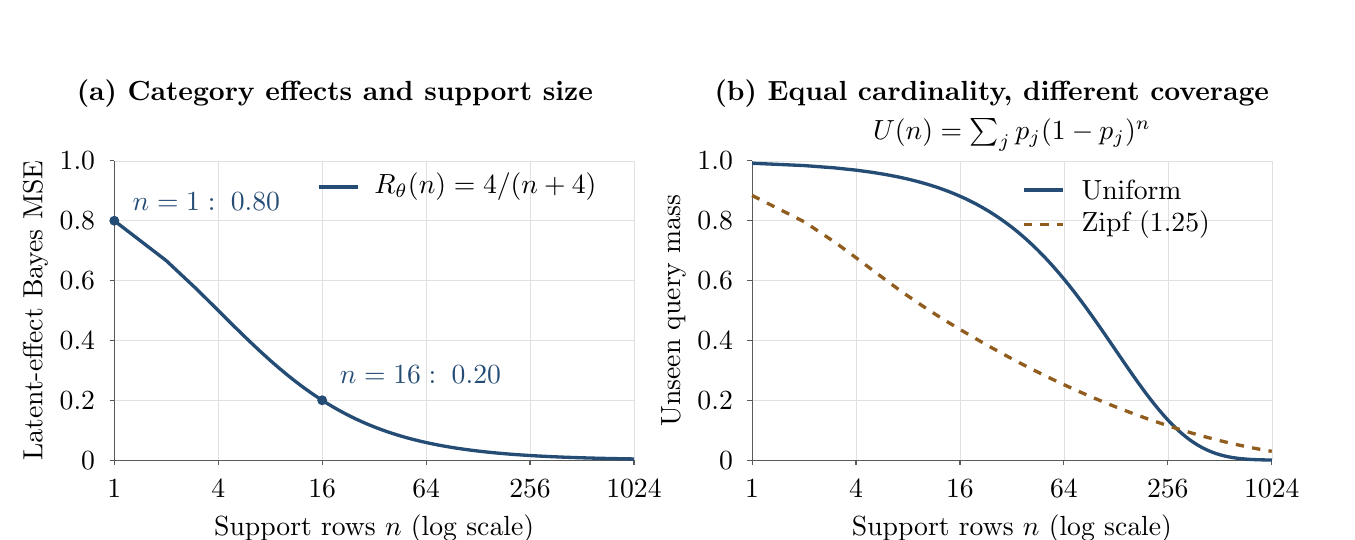
\begin{tikzpicture}[x=1cm,y=1cm,font=\fontsize{10}{12}\selectfont]
\path[use as bounding box] (0,-.05) rectangle (16.5,6.1);
\begin{scope}[shift={(1.1,1.1)}]

  \foreach \yy/\yl in {0/0,0.76/0.2,1.52/0.4,2.28/0.6,3.04/0.8,3.8/1.0} {
    \draw[black!12,very thin] (0,\yy) -- (6.6,\yy);
    \draw[black!65] (-.06,\yy) -- (0,\yy);
    \node[anchor=east] at (-.12,\yy) {\yl};
  }
  \foreach \xx/\xl in {0/1,1.32/4,2.64/16,3.96/64,5.28/256,6.6/1024} {
    \draw[black!12,very thin] (\xx,0) -- (\xx,3.8);
    \draw[black!65] (\xx,-.06) -- (\xx,0);
    \node[anchor=north] at (\xx,-.12) {\xl};
  }
  \draw[black!65] (0,3.8) -- (0,0) -- (6.6,0);
  \node[anchor=north] at (3.3,-.57) {Support rows $n$ (log scale)};

  \node[anchor=west,font=\fontsize{10}{12}\selectfont\bfseries] at (-.6,4.65)
    {(a) Category effects and support size};
  \node[rotate=90] at (-1.0,1.9) {Latent-effect Bayes MSE};
  \draw[pfnblue,line width=1.2pt] plot coordinates {(0.00000,3.04000) (0.66000,2.53333) (1.04608,2.17143) (1.32000,1.90000) (1.53247,1.68889) (1.70608,1.52000) (1.85285,1.38182) (1.98000,1.26667) (2.09215,1.16923) (2.19247,1.08571) (2.28322,1.01333) (2.36608,0.95000) (2.44229,0.89412) (2.51285,0.84444) (2.57855,0.80000) (2.64000,0.76000) (2.69773,0.72381) (2.75215,0.69091) (2.80363,0.66087) (2.85247,0.63333) (2.89893,0.60800) (2.98555,0.56296) (3.02608,0.54286) (3.06495,0.52414) (3.13823,0.49032) (3.20627,0.46061) (3.23855,0.44706) (3.30000,0.42222) (3.35773,0.40000) (3.41215,0.38000) (3.46363,0.36190) (3.51247,0.34545) (3.58133,0.32340) (3.62462,0.31020) (3.68608,0.29231) (3.74380,0.27636) (3.79823,0.26207) (3.84971,0.24918) (3.89855,0.23750) (3.96000,0.22353) (4.01773,0.21111) (4.07215,0.20000) (4.12363,0.19000) (4.18430,0.17882) (4.23020,0.17079) (4.29514,0.16000) (4.34608,0.15200) (4.40380,0.14340) (4.45823,0.13571) (4.50971,0.12881) (4.56645,0.12160) (4.62000,0.11515) (4.67773,0.10857) (4.73215,0.10270) (4.78363,0.09744) (4.83841,0.09212) (4.89578,0.08686) (4.94990,0.08216) (5.00608,0.07755) (5.05912,0.07343) (5.11381,0.06941) (5.16971,0.06552) (5.22645,0.06179) (5.28000,0.05846) (5.33422,0.05527) (5.38884,0.05223) (5.44363,0.04935) (5.50136,0.04648) (5.55578,0.04393) (5.60990,0.04153) (5.66608,0.03918) (5.71912,0.03707) (5.77602,0.03494) (5.82971,0.03304) (5.88448,0.03121) (5.94000,0.02946) (5.99422,0.02784) (6.05050,0.02625) (6.10520,0.02480) (6.15988,0.02342) (6.21439,0.02213) (6.26990,0.02088) (6.32483,0.01971) (6.38029,0.01860) (6.43491,0.01757) (6.48971,0.01659) (6.54547,0.01565) (6.60000,0.01479)};
  \draw[pfnblue,line width=1.2pt] (2.6,3.47) -- (3.1,3.47);
  \node[anchor=west] at (3.18,3.47) {$R_\theta(n)=4/(n+4)$};
  \fill[pfnblue] (0,3.04) circle (1.8pt);
  \node[anchor=south west,text=pfnblue] at (.11,3.04) {$n=1:\;0.80$};
  \fill[pfnblue] (2.64,.76) circle (1.8pt);
  \node[anchor=south west,text=pfnblue] at (2.74,.85) {$n=16:\;0.20$};
\end{scope}
\begin{scope}[shift={(9.2,1.1)}]

  \foreach \yy/\yl in {0/0,0.76/0.2,1.52/0.4,2.28/0.6,3.04/0.8,3.8/1.0} {
    \draw[black!12,very thin] (0,\yy) -- (6.6,\yy);
    \draw[black!65] (-.06,\yy) -- (0,\yy);
    \node[anchor=east] at (-.12,\yy) {\yl};
  }
  \foreach \xx/\xl in {0/1,1.32/4,2.64/16,3.96/64,5.28/256,6.6/1024} {
    \draw[black!12,very thin] (\xx,0) -- (\xx,3.8);
    \draw[black!65] (\xx,-.06) -- (\xx,0);
    \node[anchor=north] at (\xx,-.12) {\xl};
  }
  \draw[black!65] (0,3.8) -- (0,0) -- (6.6,0);
  \node[anchor=north] at (3.3,-.57) {Support rows $n$ (log scale)};

  \node[anchor=west,font=\fontsize{10}{12}\selectfont\bfseries] at (-.6,4.65)
    {(b) Equal cardinality, different coverage};
  \node at (3.3,4.13) {$U(n)=\sum_j p_j(1-p_j)^n$};
  \node[rotate=90] at (-1.0,1.9) {Unseen query mass};
  \draw[pfnblue,line width=1.2pt] plot coordinates {(0.00000,3.77031) (0.66000,3.74086) (1.04608,3.71163) (1.32000,3.68263) (1.53247,3.65386) (1.70608,3.62532) (1.85285,3.59700) (1.98000,3.56889) (2.09215,3.54101) (2.19247,3.51335) (2.28322,3.48590) (2.36608,3.45867) (2.44229,3.43165) (2.51285,3.40484) (2.57855,3.37824) (2.64000,3.35184) (2.69773,3.32566) (2.75215,3.29967) (2.80363,3.27390) (2.85247,3.24832) (2.89893,3.22294) (2.98555,3.17278) (3.02608,3.14799) (3.06495,3.12340) (3.13823,3.07479) (3.20627,3.02693) (3.23855,3.00328) (3.30000,2.95654) (3.35773,2.91052) (3.41215,2.86522) (3.46363,2.82063) (3.51247,2.77673) (3.58133,2.71216) (3.62462,2.66995) (3.68608,2.60786) (3.74380,2.54721) (3.79823,2.48798) (3.84971,2.43012) (3.89855,2.37361) (3.96000,2.30030) (4.01773,2.22925) (4.07215,2.16040) (4.12363,2.09367) (4.18430,2.01316) (4.23020,1.95098) (4.29514,1.86129) (4.34608,1.78971) (4.40380,1.70744) (4.45823,1.62895) (4.50971,1.55407) (4.56645,1.47105) (4.62000,1.39246) (4.67773,1.30778) (4.73215,1.22824) (4.78363,1.15354) (4.83841,1.07492) (4.89578,0.99384) (4.94990,0.91887) (5.00608,0.84292) (5.05912,0.77324) (5.11381,0.70379) (5.16971,0.63556) (5.22645,0.56947) (5.28000,0.51025) (5.33422,0.45362) (5.38884,0.40012) (5.44363,0.35017) (5.50136,0.30169) (5.55578,0.25992) (5.60990,0.22219) (5.66608,0.18698) (5.71912,0.15734) (5.77602,0.12933) (5.82971,0.10630) (5.88448,0.08601) (5.94000,0.06851) (5.99422,0.05415) (6.05050,0.04180) (6.10520,0.03202) (6.15988,0.02414) (6.21439,0.01792) (6.26990,0.01299) (6.32483,0.00927) (6.38029,0.00646) (6.43491,0.00444) (6.48971,0.00297) (6.54547,0.00193) (6.60000,0.00124)};
  \draw[pfnamber,line width=1.2pt,dashed] plot coordinates {(0.00000,3.36100) (0.66000,3.02787) (1.04608,2.77135) (1.32000,2.57061) (1.53247,2.41076) (1.70608,2.28111) (1.85285,2.17401) (1.98000,2.08392) (2.09215,2.00683) (2.19247,1.93981) (2.28322,1.88071) (2.36608,1.82794) (2.44229,1.78030) (2.51285,1.73690) (2.57855,1.69704) (2.64000,1.66019) (2.69773,1.62594) (2.75215,1.59394) (2.80363,1.56393) (2.85247,1.53568) (2.89893,1.50901) (2.98555,1.45981) (3.02608,1.43703) (3.06495,1.41533) (3.13823,1.37480) (3.20627,1.33764) (3.23855,1.32018) (3.30000,1.28723) (3.35773,1.25664) (3.41215,1.22812) (3.46363,1.20144) (3.51247,1.17638) (3.58133,1.14149) (3.62462,1.11981) (3.68608,1.08937) (3.74380,1.06115) (3.79823,1.03486) (3.84971,1.01028) (3.89855,0.98721) (3.96000,0.95854) (4.01773,0.93196) (4.07215,0.90722) (4.12363,0.88410) (4.18430,0.85721) (4.23020,0.83712) (4.29514,0.80906) (4.34608,0.78736) (4.40380,0.76309) (4.45823,0.74053) (4.50971,0.71946) (4.56645,0.69656) (4.62000,0.67526) (4.67773,0.65263) (4.73215,0.63161) (4.78363,0.61201) (4.83841,0.59146) (4.89578,0.57027) (4.94990,0.55061) (5.00608,0.53052) (5.05912,0.51186) (5.11381,0.49294) (5.16971,0.47394) (5.22645,0.45499) (5.28000,0.43743) (5.33422,0.41997) (5.38884,0.40271) (5.44363,0.38573) (5.50136,0.36821) (5.55578,0.35204) (5.60990,0.33630) (5.66608,0.32032) (5.71912,0.30556) (5.77602,0.29011) (5.82971,0.27588) (5.88448,0.26172) (5.94000,0.24775) (5.99422,0.23447) (6.05050,0.22107) (6.10520,0.20843) (6.15988,0.19617) (6.21439,0.18434) (6.26990,0.17269) (6.32483,0.16155) (6.38029,0.15071) (6.43491,0.14044) (6.48971,0.13053) (6.54547,0.12086) (6.60000,0.11181)};
  \draw[pfnblue,line width=1.2pt] (3.45,3.43) -- (3.95,3.43);
  \node[anchor=west] at (4.06,3.43) {Uniform};
  \draw[pfnamber,line width=1.2pt,dashed] (3.45,2.99) -- (3.95,2.99);
  \node[anchor=west] at (4.06,2.99) {Zipf ($1.25$)};
\end{scope}
\end{tikzpicture}
\caption{Exact diagnostics for the distribution of evidence in a synthetic prior. (a) For a category effect $\theta\sim\mathcal N(0,1)$ and $y_i\mid\theta\sim\mathcal N(\theta,4)$, the posterior-mean risk for $\theta$ is $4/(n+4)$; risk for a new noisy response adds $4$. (b) Support and query categories are independent draws from the same law over $128$ categories: either uniform or $p_j\propto j^{-1.25}$. Curves connect exact values at integer support sizes. Unseen query mass weights categories by their population frequency and therefore differs from the fraction of category identities absent from context. Neither calculation estimates benchmark accuracy or identifies optimal mixture weights.}
\label{fig:prior-information-diagnostics}
\end{figure}

\subsection{Choosing the mixture within the compute budget}

The first phase, P, compares eight distributions: unchanged R; R with the observation mixture; R with 20\% F; R with 15\% H; R with 10\% S; R with 5\% I; full Q with identity observation; and full Q with the observation mixture. The individual mechanism additions use identity observation. Each arm uses seeds 0 and 1 and a 300 GPU-hour allowance per seed, totaling 4,800 hours. Classification and regression share that allowance. This phase tests the additions separately, then asks whether their combination and the observation process produce further benefit.

Phase M varies the graph share across $.70,.50,.30$, preserving the F/H/S/I ratio $4:3:2:1$ in the remainder. The vectors are $(.70,.12,.09,.06,.03)$, $(.50,.20,.15,.10,.05)$ and $(.30,.28,.21,.14,.07)$. All three use the same observation law and fresh seeds 2 and 3 at 300 hours per seed, totaling 1,800 hours. Fresh seeds prevent the central mixture from repeating the identical Q run in phase P. Before launch, one recorded slot may instead test complexity-on/off or filter sensitivity if the diagnostics make that uncertainty more pressing. The replacement uses the existing allowance. Removing a family likewise creates a newly identified candidate, whose weights must be recorded before the run.

Phase A crosses R and the selected challenger with the authored compressed architecture and a compact persistent-cell alternative. Four cells, two seeds and 400 hours per run require 3,200 hours. Both architectures are implemented. Their different parameter counts make this an equal-cost system comparison; it does not isolate topology at equal model size. Phase V then confirms the complete reference and finalist using fresh seeds 4 and 5 at 700 hours per run, totaling 2,800 hours.

The remaining 2,400 hours form phase F: three continuations from a common standard parent, each using seeds 6 and 7 and 400 hours per seed. The continuations are standard replay, fraud training with reservoir-plus-observed-positive context, and fraud training with the full selector. Both fraud arms hide H, retain the legal label-availability rules and use correct population weights.

The five phases use 15,000 GPU-hours and replace the earlier screening allocation in Section~\ref{sec:revised-budget}. Optimizer, head, codec, length-scaling and sharing settings remain fixed; separate sweeps of these factors are deferred. The existing 10,000-hour size/bridge phase is retained: two sizes by two seeds at 500 hours, reference and challenger bridges at 3,000 hours each, and two 1,000-hour runs to resolve remaining questions. R reaches the longer bridge even if a small pilot ranks it lower, since early rankings may change with training scale. Including final training, evaluation and reserve, the project remains within 50,000 hours.

\paragraph{Real-data selection.}
The search requires separate development, confirmation and final evaluation data. Before training, register at least twenty independent dataset lineages for each of binary classification, multiclass classification and regression in the development panel, and at least ten per task type in the confirmation panel. These are coverage targets, not a power calculation. The panels should span the intended feature types, widths, context sizes and missingness patterns. Duplicates, derived targets and related datasets belong to the same lineage. Official final benchmark folds and customer evaluation periods remain outside mixture selection. If sufficiently disjoint data are unavailable, the scope of the claim must be reduced rather than the final benchmark reused.

For each dataset, average folds within training seed, then compare paired seed averages. The primary normalized improvement is reduction in log loss for classification and MSE for regression relative to the reference, divided by the constant-predictor loss estimated from that dataset's training split. Fix denominator floors before evaluation and report raw metrics as well. Average datasets equally within each task type and the three task types equally overall. Report binary AUC, multiclass log loss, regression RMSE and distributional calibration separately so an aggregate cannot hide a regression in one objective.

Development results rank the exploratory arms, with uncertainty retained. A finalist is assessed on the untouched confirmation panel: the 95\% paired dataset-lineage bootstrap interval must exclude zero overall improvement, and its lower bound must exceed $-.005$ normalized units for each task type. The .005 tolerance is a declared design choice. All paired predictions are resampled together by lineage, using 10,000 bootstrap draws. Training-seed variation is reported separately because two seeds estimate it poorly. If no candidate passes, the search has not selected a stronger bank. Once confirmation results are repeatedly used to revise the recipe, that panel becomes development data and another holdout is required.

Preprocessing, support size and inference policy remain fixed during prior selection. The surviving systems are then compared for cold context setup, cached GPU batch prediction, peak memory and accuracy at 1/4/8 views. Predictive performance takes priority on the measured accuracy--latency frontier. A prior changes what the model learns, not its arithmetic at a fixed shape. It can improve latency indirectly if the resulting model reaches comparable accuracy with less context, fewer views, a smaller architecture or a more efficient implementation.

For reproducibility, the classification constant predictor uses training class counts with Jeffreys smoothing, $(n_k+1/2)/(n+K/2)$. Regression losses in the search objective are computed after the existing support-only target standardization. For both objectives, divide the paired loss reduction by $\max(10^{-6},L_0)$, where $L_0$ is the training loss of the corresponding constant predictor in those units. This fixes the denominator before query evaluation. Raw-unit regression RMSE remains a separate reported endpoint. Bootstrap conclusions are conditional on the trained checkpoints; the small number of training seeds remains a distinct source of uncertainty.

\paragraph{Cheap diagnostics before GPU screens.}
Before GPU training, the generators are audited on at least 1,000 independent worlds per family and stage, stratified by observation mode and task type. The audit records actual informative dimensions, type masks, support occupancy, missingness, coarsening contradictions, class frequencies and rejection costs, and checks query-label independence, category renaming and calibration separation.

A smaller stratified subset is used for finite-context learning curves. Ridge/logistic, kernel or nearest-neighbor and tree learners receive the same support; any learner selection uses internal support cross-validation, and a separate query set measures performance. These losses are attainable reference values, not Bayes risks. Teacher comparisons retain negative estimated gaps and uncertainty, and failure of one learner is not a reason to remove a whole prior family.

The planner in \path{scripts/plan_prior_selection.py} reads \path{research/specs/prior_selection_v1.json} and produces forty trial records with their costs, mixture exposure and unresolved dependencies. The operating instructions are in \path{docs/prior_selection.md}. These artifacts make the experiment reviewable, but do not launch training. The sampler, common laws, compact architecture and training path are now implemented. \path{scripts/materialize_prior_selection.py} writes the runnable configurations for each phase, and \path{scripts/submit_training.py} submits a resolved run with a scheduler wall-time limit. Stage costs and real-data outcomes still have to be measured.


\section{Implemented reference and authored standard generators}
\label{app:staticrecipe}

The executable pilot begins with the released TabICLv2 generator and adds hierarchical category tasks on eligible draws. Its sampler is the reference implementation against which the proposed challenger will be developed. This choice separates the breadth of the reference distribution from the specific question of whether repeated identities improve inference. We describe the reference mixture and its generation procedure first, then give the complete authored P0/P1/P4 distribution used in the replacement comparisons. Its configuration is \path{research/specs/static_recipe_v3.json}. Unless a draw is identified as row-specific, the authored generator samples it once per world and shares the resulting parameters across calibration, support and query records.

The authored bank covers smooth responses, sharp boundaries, joint causal dependence, local similarity, category pooling and count or amount outcomes. Two further comparisons examine how these tasks are learned: context conditioning changes mechanism complexity while holding the rest of the bank fixed, whereas conditional-label supervision changes the estimator of the training objective. They are evaluated separately from changes to the mixture itself.

\subsection{Reference prior and proposed extensions}
\label{sec:prior-revision}

The reason for retaining the open reference is its range of compositional structure. TabICLv2 combines eight function families in vector-valued graphs with structured hyperparameter sampling \cite{tabicl2}. The authored \texttt{static-v3-base} SCM instead uses four node-function families and at most sixteen observed informative causal nodes; additional columns are often proxies or distractors. It therefore serves as a controlled alternative whose transfer must be compared with that of the broader reference.

Arm R uses an unchanged source revision of the released generator. The first extension, G, introduces hierarchical-category tasks P1 through a 95\% reference and 5\% P1 draw, conditional on a task type and shape sampled \emph{before} the generator is selected. Eligibility requires $F\geq8$; the P1 share returns to R on narrower tasks. Extension C separately introduces 5\% count/amount P4 into a 95\% reference mixture for binary/regression tasks with $F\geq4$, using 100\% R elsewhere.

These comparisons hold the classification/regression mix, context sizes and feature widths fixed. Realized proportions are recorded after eligibility and filtering, since nominal branch probabilities alone do not describe the accepted distribution. If both additions are supported by their separate experiments, a 90/5/5 mixture can be tested on shapes where both are legal, again returning each ineligible component's share to R. The small initial additions make the comparison interpretable; they are pilot choices rather than estimated optimal weights.

The adapter in \path{reference_prior.py} implements this ordering by invoking the pinned source and recording raw proposals, rejection reasons and realized shapes. R keeps its released filters. P1 and P4 receive the previously selected task, shape and class budget, and use validity-only acceptance. Applying the reference teacher filter to either addition would introduce a further change to the experiment.

The generator interface and batching also delimit the comparison with the published system. Native R returns numerically encoded columns without categorical type flags. Explicit training of the nominal encoder therefore comes mainly from P1 and separately typed tasks; model preprocessing is specified independently of the native generator.

The current trainer requests one episode at a time. Although this preserves the per-table sampling procedure, it omits the first-stage grouping in which four tables share their row count, support split and requested width. Class budgets and graphs are sampled separately even within that group. The batch API preserves the released grouping, while the later stages already use groups of one.

The earlier development plan addressed category occupancy and conditional uncertainty, followed by zeros, exposure and dispersion. Its G/C controls remain specified here; the current funded comparisons are those in Section~\ref{sec:prior-selection}. Results within the relevant real-data strata determine whether either addition merits a larger share. Structured missingness and coarsening remain important coverage controls, although they are established prior ingredients. Context caps, conditional-label losses, adaptive weights and real-data continuation are treated as separate factors. If G or C fails its comparison, the corresponding choice remains R; the result does not trigger an open-ended search through additional families.

\paragraph{Native and expanded envelopes.} The released curriculum increases the number of rows from a fixed 1,024 in the first stage to 400--10,240 in the second and 400--60,000 in the third. Native R permits at most 100 features and ten class-budget slots, with additional width caps for long tables. The candidate retains this law on 80\% of later-stage requests. The other 20\% use maxima of 256 features and 32 classes in stage two, and 512 features and 256 classes in stage three. These settings are recorded as changes to the generator distribution.

The larger limits describe requests, not guaranteed coverage. Constant-column removal, class realization and native split repair still determine the accepted table. In one local diagnostic, a request for 64 classes yielded 25 observed classes after twelve raw attempts. Decisions to expand the range or commit a long run therefore require realized class and width histograms. Forcing query-class coverage or padding labels would alter the sampling law and would not establish that a 256-class task had been generated.


\subsection{Generating a standard training episode}
\label{sec:prior-walkthrough}

A standard episode starts with the task and dimensions: classification or regression, curriculum stage, total rows, support split, requested feature count and, for classification, class budget. The R/P1 branch is drawn only after these choices. Eligible P1 tasks inherit the complete specification; a P1 selection below the minimum width of eight returns to R. Fixing these quantities first keeps a generator's preference for particular shapes from changing its assigned share.

\paragraph{R: draw a graph, evaluate a table, then apply the released acceptance law.}
R generates features and outcomes jointly through a hidden computation graph. The pinned implementation proceeds through the following stages, retaining the outer task and shape while it searches for an accepted table.
\begin{enumerate}
\item \textbf{Draw a raw-table specification.} Feature types, category cardinalities and shared distributional settings are sampled for the raw table. The response type is already fixed by the classification/regression task. Compatibility behavior in the released source limits native feature-category cardinalities to at most nine.
\item \textbf{Construct a hidden acyclic graph.} A graph with 2--32 nodes receives the requested observed features and target as node outputs. Several columns may come from one node, and some nodes remain unobserved. Graphs and column placements are redrawn until the features and target share ancestors. This screen imposes a structural opportunity for dependence; it does not identify causal relationships in a real table.
\item \textbf{Give nodes functions.} Roots receive random vector inputs. The remaining nodes concatenate or aggregate parent vectors and transform them with sampled MLPs, oblivious-tree ensembles, discretization, linear or quadratic maps, random-Fourier GP maps, EM-like assignments, or products. Different function types can coexist in the same graph. Hidden node states can also have more dimensions than the columns ultimately observed.
\item \textbf{Evaluate all requested rows.} Topological traversal produces numerical and categorical outputs through sampled converters, while passing converted hidden vectors to descendants. The raw table shares its parameters and fitted transformations. Many transformations are fitted on the generated rows themselves, because the released configuration has no separate IID fit-only pass. Roots, hidden dimensions and categorical draws provide variation even though optional extra additive Gaussian node noise is disabled by default.
\item \textbf{Render and test the table.} Native values are clipped and standardized, columns and class IDs are permuted, and constant features are removed. A table with no remaining features is rejected. Classification allows up to ten row permutations to obtain identical observed class sets in support and query, with at least two labels. A 25-tree, depth-six ExtraTrees OOB test then uses 200 bootstrap resamples to reject insufficiently predictable tables; the optional too-easy filter is disabled. Rejection starts a new internal-world draw under the same outer task, shape and source.
\item \textbf{Return safe inputs and separate targets.} The accepted rows form the support and query sets. Native categorical columns are already numerically encoded and carry no type flags, so the local model receives this numerical interface through its support-only codec. The forward arguments contain neither the hidden graph nor the query labels or rejection diagnostics.
\end{enumerate}

These stages are executed by the retained generator through \path{reference_prior.py}. Within \path{third_party/tabicl_reference/src/tabicl/prior/}, \path{_dataset.py} specifies shapes and acceptance, \path{_graph_scm.py} constructs raw tables, and \path{graph_lib/} supplies graphs, node functions and converters. The source manifest fixes all of these files: changes to table-wide transformations, split repair or filtering would change the accepted distribution even if the list of graph functions stayed the same.

\begin{figure}[htbp]
\centering
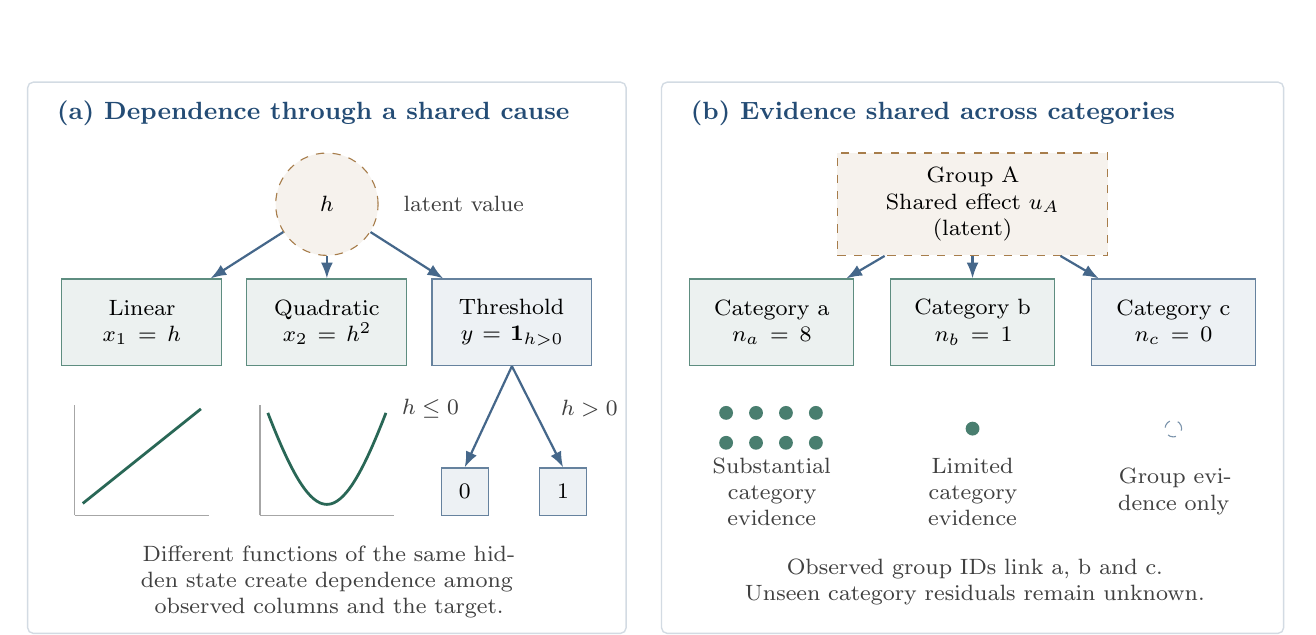
\begin{tikzpicture}[x=1cm,y=1cm,
  font=\small,
  panel/.style={draw=pfnblue!20,line width=.5pt,rounded corners=2pt,fill=white},
  title/.style={font=\small\bfseries,text=pfnblue,anchor=west},
  note/.style={font=\footnotesize,align=center,text=black!75},
  process/.style={font=\footnotesize,draw=pfnblue!70,fill=pfnblue!5,rounded corners=2pt,align=center,inner sep=5pt},
  support/.style={font=\footnotesize,draw=pfngreen!75,fill=pfngreen!9,align=center,inner sep=4pt},
  query/.style={font=\footnotesize,draw=pfnblue!70,fill=pfnblue!8,align=center,inner sep=4pt},
  hidden/.style={font=\footnotesize,draw=pfnamber!80,fill=pfnamber!8,align=center,inner sep=4pt,dashed},
  flow/.style={-{Latex[length=2mm]},draw=pfnblue!85,line width=.8pt},
  target/.style={-{Latex[length=2mm]},draw=pfnamber!90,line width=.8pt,dashed},
  reuse/.style={-{Latex[length=2mm]},draw=pfngreen!90,line width=.8pt,dashed}]

\path[use as bounding box] (0,.2) rectangle (16,-7.15);
\draw[panel] (0,0) rectangle (7.6,-7);
\draw[panel] (8.05,0) rectangle (15.95,-7);
\node[title] at (.25,-.4) {(a) Dependence through a shared cause};
\node[title] at (8.3,-.4) {(b) Evidence shared across categories};
\node[hidden,circle,minimum size=13mm] (h) at (3.8,-1.55) {$h$};
\node[note,anchor=west] at (4.65,-1.55) {latent value};
\node[support,text width=1.75cm,minimum height=11mm] (linear) at (1.45,-3.05)
  {Linear\\$x_1=h$};
\node[support,text width=1.75cm,minimum height=11mm] (quad) at (3.8,-3.05)
  {Quadratic\\$x_2=h^2$};
\node[query,text width=1.75cm,minimum height=11mm] (threshold) at (6.15,-3.05)
  {Threshold\\$y=\ind_{h>0}$};
\draw[flow] (h)--(linear);
\draw[flow] (h)--(quad);
\draw[flow] (h)--(threshold);
\draw[black!35] (.6,-5.5)--(2.3,-5.5);
\draw[black!35] (.6,-5.5)--(.6,-4.1);
\draw[pfngreen,line width=1pt] (.7,-5.35)--(2.2,-4.15);
\draw[black!35] (2.95,-5.5)--(4.65,-5.5);
\draw[black!35] (2.95,-5.5)--(2.95,-4.1);
\draw[pfngreen,line width=1pt] (3.05,-4.2) .. controls (3.65,-5.75) and (3.95,-5.75) .. (4.55,-4.2);
\node[query,minimum width=6mm,minimum height=6mm] (leaf0) at (5.55,-5.2) {$0$};
\node[query,minimum width=6mm,minimum height=6mm] (leaf1) at (6.8,-5.2) {$1$};
\draw[flow] (threshold.south)--(leaf0.north);
\draw[flow] (threshold.south)--(leaf1.north);
\node[note,anchor=east] at (5.6,-4.15) {$h\leq0$};
\node[note,anchor=west] at (6.65,-4.15) {$h>0$};
\node[note,text width=6.8cm] at (3.8,-6.35)
  {Different functions of the same hidden state create dependence among observed columns and the target.};
\node[hidden,text width=3.15cm,minimum height=13mm] (group) at (12,-1.55)
  {Group A\\Shared effect $u_A$\\(latent)};
\node[support,text width=1.8cm,minimum height=11mm] (a) at (9.45,-3.05)
  {Category a\\$n_a=8$};
\node[support,text width=1.8cm,minimum height=11mm] (b) at (12,-3.05)
  {Category b\\$n_b=1$};
\node[query,text width=1.8cm,minimum height=11mm] (c) at (14.55,-3.05)
  {Category c\\$n_c=0$};
\draw[flow] (group)--(a);
\draw[flow] (group)--(b);
\draw[flow] (group)--(c);
\foreach \rr in {0,1}
  \foreach \cc in {0,1,2,3}
    \fill[pfngreen!85] (8.87+.38*\cc,-4.2-.38*\rr) circle (2.5pt);
\fill[pfngreen!85] (12,-4.4) circle (2.5pt);
\draw[draw=pfnblue!60,dashed] (14.55,-4.4) circle (3pt);
\node[note,text width=2.1cm] at (9.45,-5.2) {Substantial category evidence};
\node[note,text width=2.1cm] at (12,-5.2) {Limited category evidence};
\node[note,text width=2.1cm] at (14.55,-5.2) {Group evidence only};
\node[note,text width=7.15cm] at (12,-6.35)
  {Observed group IDs link a, b and c.\\Unseen category residuals remain unknown.};

\end{tikzpicture}
\caption{Illustrative structures in the standard bank. (a) A common latent ancestor induces dependence among features and the target. (b) A shared group effect allows information to transfer to categories with few or no support observations when an observed group identifier or metadata exposes that relationship. Counts denote support rows. These are schematic examples, rather than outputs of the native generator; latent effects are not model inputs.}
\label{fig:prior-mechanisms}
\end{figure}

The left-hand schematic can be illustrated by four hand-chosen latent values. The resulting table shows how a common hidden mechanism induces dependence among two columns and the target. All four outcomes are known to the generator, but only support outcomes enter the predictor. This example deliberately omits the native row count, vector mechanisms and acceptance filter.
\begin{center}\small
\begin{tabular}{@{}lrrl@{}}
\toprule Partition & Visible $x_1$ & Visible $x_2$ & Target $y$\\
\midrule
Support & $-1$ & $1$ & $0$, visible\\
Support & $1$ & $1$ & $1$, visible\\
Query & $-.5$ & $.25$ & $0$, withheld for loss\\
Query & $.5$ & $.25$ & $1$, withheld for loss\\
\bottomrule
\end{tabular}
\end{center}

\paragraph{P1: entity and group effects.}
P1 makes repeated identities informative. Observations of the same category reveal a shared effect, while group membership and observed metadata provide a basis for prediction when few direct observations are available.
\begin{enumerate}
\item Four requested columns are reserved for entity ID, parent-group ID and two observed metadata coordinates. The authored feature factory generates the remaining $F-4$ columns. Separate streams supply 4,096 internal calibration rows, support rows and query rows; calibration records fit the generator and never become additional model context.
\item The entity catalog has discrete-log-uniform size from eight through $\min(4096,\max(16,2n_s))$, with an integer group count between two and $\min(32,\max(2,E/2))$. Entity frequencies are uniform with probability .2 and otherwise follow a randomly ranked power law. This produces both balanced catalogs and catalogs with a long tail of rarely observed entities.
\item Metadata, an intercept and optional slopes are drawn once for each entity. The intercept combines a component predictable from metadata with a hidden component. Entities in the same group also share a group intercept. Section~\ref{sec:p1-full} gives the scales and probabilities.
\item Each row samples its entity ID from the fixed frequency law. Its score combines a common GAM, the entity and group intercepts, and entity-specific slopes on up to two ordinary coordinates. For output coordinate $k$, this gives
\[
 s_k(v,e)=b_k(v)+a_{e,k}+g_{\operatorname{group}(e),k}
                    +\beta_{e,k}^{\top}v_{1:d},\qquad d=\min(2,d_{\rm active}).
\]
The coordinates $v$ are latent features before rendering, masking and column permutation.
\item Calibration fixes the response conversion, after which the chosen binary, multiclass or regression outcomes are sampled. Common rendering and missingness rules produce the observed table. IDs retain their nominal type, and support and query share the same effects. This branch is accepted without the native R teacher filter.
\end{enumerate}

In the illustration, eight observations of category a provide direct information about its effect. For the absent category c, prediction instead relies on its group, metadata and other features, with uncertainty remaining about the hidden residual. The shared structure supports \emph{partial pooling} without requiring equal effects for all entities. The network is trained on this inference problem across tasks; no programmed partial-pooling estimator is inserted into it. The implementation is in \path{static_prior.py}, particularly \texttt{\_p1()}, the feature factory and the response compiler.

Missingness is underrepresented in the executable R/P1 pilot, motivating the observation law in Section~\ref{sec:prior-selection}. Native R adds no deliberate NaN corruption. P1 enables independent MCAR masking on 30\% of its tasks at cell-mask rate $U(.01,.20)$; its other tasks have no such masking. After width eligibility is accounted for, approximately 1.402\% of all standard tasks enable masking, or 897,454 tasks in the 64 million-task plan, in expectation. These counts describe training exposure, not measured robustness. The finance specialist has the structured missingness mechanisms specified below, but that separate continuation cannot improve the retained standard checkpoint. Evaluation must distinguish accepting missing inputs from predicting reliably under different missingness mechanisms.

\subsection{Authored-bank control: mixture and variants}

The authored replacement control combines P0, P1 and P4 through the following \emph{marginal} probabilities. Within P0, the five subfamilies have conditional probabilities of 20/25/30/15/10 percent, which sum to one. Multiplying these by P0's 85\% share gives the table entries.
\begin{table}[ht]
\centering\small
\begin{tabularx}{\linewidth}{@{}lrY@{}}
\toprule
Generator & Episode mass & Intended inference capability\\
\midrule
P0 linear/GLM/GAM and interactions & 17.00\% & Sparse/additive effects and low-order composition\\
P0 sharp tree and tree-ensemble functions & 21.25\% & Discontinuities, thresholds and regime boundaries\\
P0 heterogeneous joint SCMs & 25.50\% & Latent causes, redundant observations and arbitrary target position\\
P0 local/kernel functions & 12.75\% & Similarity, local smoothness and anisotropy\\
P0 gated regime compositions & 8.50\% & Context-dependent mechanisms with shared structure\\
P1 hierarchical categorical effects & 10.00\% & Partial pooling, rare levels and meaningful category metadata\\
P4 counts and compound amounts & 5.00\% & Zeros, dispersion, exposure and heavy positive tails\\
\bottomrule
\end{tabularx}
\caption{Starting probabilities for the authored-bank control. Missingness, rendering, class prevalence and observation coarsening are conditional modifiers.}
\end{table}

The initial replacement comparison uses \texttt{static-v3-base}, with fixed mixture weights, independently sampled mechanism complexity, hard labels, validity-only filtering and no auxiliary loss. \texttt{static-v3-context} changes only the specified 90\% context-capped/10\% base-replay rule. Conditional-distribution losses form a further, separate comparison. Introducing these changes one at a time permits selection of a confirmed combination on evidence rather than on the apparent realism of its ingredients.

\subsection{Sampling conventions and base task shapes}

The distributions below use $\operatorname{RU}(a,b)$ for a uniform integer on the inclusive set $\{a,\ldots,b\}$ and $\operatorname{LU}(a,b)=\exp U(\log a,\log b)$ for a positive real. Their discrete-log-uniform counterpart is
\[
\operatorname{DLU}(a,b)=\min\{b,\max\{a,\lfloor\exp U(\log a,\log(b+1))\rfloor\}\}.
\]
Integer bounds are inclusive; continuous uniforms are half-open at the upper endpoint. Empirical quantiles use the NumPy convention of linear interpolation between neighboring order statistics, and calibration moments use population denominators without degrees-of-freedom corrections. Equality follows the left child at a numerical tree split and the upper bin at a quantile-category boundary. Unless probabilities are given, ``choose'' denotes uniform sampling without replacement.

The numerical conventions also fix degenerate cases. Empty interactions contribute zero, and coefficient normalization divides by $\max(10^{-12},\|w\|_2)$ so that an all-zero vector remains zero. Categorical probabilities are normalized in float64; softmax subtracts the largest logit. Generation and calibration are initially evaluated in float64, with model inputs cast afterward. Independent counter-based streams named \texttt{shape}, \texttt{parameters}, \texttt{calibration}, \texttt{support}, \texttt{query}, \texttt{labels}, and \texttt{rendering} include world ID and retry number in every key.

The authored standard profile balances binary classification, multiclass classification and regression; finance has its own observation and selection process. Family probabilities are $.85/.10/.05$ for P0/P1/P4. Because P4 chooses binary classification with probability $.2$ and regression with $.8$, the corresponding task probabilities for P0 and P1 are
\[
(p_{\rm bin},p_{\rm multi},p_{\rm reg})=
\left(\frac{1/3-.05(.2)}{.95},\frac{1/3}{.95},
\frac{1/3-.05(.8)}{.95}\right)
\approx(.340350877,.350877193,.308771930),
\]
so each head receives exactly one-third of the nominal standard-profile episode mass. Support sets with absent classes are accepted by default. Reports of proposed and accepted distributions must still include arithmetic failures.

Context sizes vary within three equally likely bins: $[32,127]$, $[128,511]$, and $[512,2048]$. Support size is uniform within the selected bin, and query size is $n_q=\min(128,\max(16,\lfloor n_s/4\rfloor))$. Total width $p$ is drawn from $\{4,8,16,32,64,128\}$ with probabilities $(.10,.15,.20,.25,.15,.15)$. Reserved columns impose a minimum width: P1 replaces $p$ by $\max(p,8)$ and P4 by $\max(p,4)$.

Binary tasks use $K=2$. Multiclass tasks draw $K=\operatorname{RU}(3,10)$, replace $n_s$ by $\max(n_s,16K)$ and recompute $n_q$. This support floor couples task complexity to context size without making class coverage a requirement of the declared-vocabulary protocol. It also changes the realized context histogram relative to the proposed bin weights, so both are recorded. Dimensions count actual data, excluding hidden padding.

An independent pool of $4096$ calibration rows fixes the generator's constants before model context is constructed. These rows are neither support nor scored queries, and their labels remain outside the learner interface. The returned record contains the typed table, support/query indices, support labels and task kind; a separate evaluator object holds query labels, world parameters, achieved calibration statistics and provenance. Category IDs retain their nominal meaning. Model preprocessing uses support alone, while calibration constants remain internal sampler parameters.

\subsection{Shared features and the observation process}

The shared feature factory varies both the number of informative coordinates and their representation. For P0 outside the SCM branch, the informative count is $d$: with probability $.75$, $d=\operatorname{DLU}(1,\min(p,16))$; otherwise $d=\operatorname{RU}(\lceil p/3\rceil,p)$. P1/P4 use the same law on their nonreserved width. A world-level categorical fraction $r_c\in\{0,.25,.5,1\}$ has probabilities $(.35,.30,.25,.10)$, and each base coordinate independently becomes categorical with probability $r_c$.

Numerical features combine local correlation with occasional shared scale variation. Their world correlation is $r\in\{0,.3,.8\}$ with probabilities $(.4,.4,.2)$; after a random permutation, numerical indices form consecutive blocks of four. Each row draws a standard normal $u_b$ for each block and independent $\epsilon_j\sim N(0,1)$, giving $v_j=\sqrt r\,u_b+\sqrt{1-r}\,\epsilon_j$. With probability $.2$ per world, every numerical coordinate in a row is additionally multiplied by $\sqrt{5/\chi^2_5}$ using a single row-specific denominator. This shared scale produces heavy-tailed geometry with bounded degrees of freedom, rather than independent marginal noise.

Categorical coordinates represent nominal effects. Their cardinality $C$ follows
\[ C\in\{2,3,5,10,32,128\},\qquad P(C)=(.25,.15,.20,.20,.15,.05).\] Frequencies are proportional to $r^{-a}$ after drawing exponent $a=U(0,1.5)$ and permuting ranks. Each category receives a fixed effect $e_c\sim N(0,1)$, centered and scaled by its exact frequency-weighted mean and variance, with a variance floor of $10^{-12}$. Rows draw categories from those fixed frequencies. The generating functions use $v_j=e_c$, whereas the learner observes a separately permuted categorical code. No arithmetic is performed on that code. The construction thus assigns effects to nominal categories, unlike an ordered discretization of Gaussian values.

The remaining $p-d$ columns distinguish proxies from unrelated distractors. Independently for each column, probability $.3$ selects a copy of a uniformly chosen informative coordinate. A numerical copy adds $N(0,\sigma^2)$ noise with $\sigma=\operatorname{LU}(.01,.3)$; a categorical copy replaces its category by an independent frequency draw with probability $.05$ per row. The other branch draws a fresh factory coordinate without a factor shared with informative coordinates.

Observation maps separate latent coordinates used by the score from the values available to the learner. Each numerical coordinate receives one fixed transformation: identity with probability $.50$, $\operatorname{asinh}(v)$ with $.15$, $\operatorname{sign}(v)|v|^q$ with probability $.20$ and exponent $q=\operatorname{LU}(.3,3)$, or $\exp(\operatorname{clip}(v,-5,5))$ with $.15$. The resulting value is $x=A T(v)+B$, with $A=\operatorname{LU}(.1,10)$ and $B\sim N(0,3^2)$, while the score continues to use prerendered $v$. These maps can be invertible or clipped.

Quantization adds a separate source of information loss. Independently, with probability $.25$ per world, the generator chooses $\min(p_{\rm num},\lfloor p/4\rfloor)$ numerical columns, where $p_{\rm num}$ is the available count, and rounds each to the nearest grid point, with ties to even. Grid width is $\operatorname{LU}(.05,.5)$ times that column's calibration standard deviation. Constant columns remain valid, including those arising from a nonlinear function or a particular categorical draw.

The baseline observation process includes simple missingness: with probability $.70$ no cells are masked; otherwise a world rate $m=U(.01,.20)$ gives independent cell-masking probability $m$. An explicit mask accompanies the values. MAR/MNAR mechanisms and query shifts are separate named ablations. Columns and category codes are permuted once per world and used consistently across splits, with no transformation inferred from query outcomes.

\subsection{Response distributions and task construction}

P0/P1 share a response compiler so that differences among their mechanisms do not require different task definitions. Each first supplies a fixed score function $F$, with one output for regression/binary classification and $K$ for multiclass. Calibration centers each output and divides it by its standard deviation with denominator $\max(10^{-6},s)$. A variance below $10^{-12}$ produces a zero standardized output and a logged degeneracy. These operations scale an internal function; they do not normalize emitted targets using query labels.

Regression spans null through noiseless relations. The respective probabilities of null, weak, medium, strong and noiseless signal are $(.05,.20,.45,.25,.05)$, with $\rho=0$, $U(.02,.2)$, $U(.2,.7)$, $U(.7,.98)$, or $1$. For $0<\rho\leq1$, the pretransform response is
\[
w=s(v)+\sqrt{(1-\rho)/\rho}\,h(v)\epsilon.
\]
The null class instead uses $w=\epsilon$ and removes structural paths from the target into features. A world selects one noise family: standard normal with probability $.60$, variance-normalized Student-$t_5$ with $.20$, variance-one Laplace with $.10$, or the mixture $.9N(0,.5^2)+.1N(0,2^2)$ divided by $\sqrt{.625}$ with $.10$. Individual noise draws vary by row.

Noise is homoscedastic with probability $.6$, in which case $h=1$. Otherwise one informative coordinate determines $h_0=\exp(.5\tanh(v_j))$, normalized by $\sqrt{\operatorname{mean}_{C}(h_0^2)}$. Thus $\rho$ approximately calibrates the \emph{pretransform} variance fraction; it need not equal the final observed $R^2$.

The final response transformation is identity, signed $\log(1+|w|)$, or $\exp(\operatorname{clip}(w,-8,8))$ with probabilities $(.75,.15,.10)$. Output scale $B=\operatorname{LU}(.1,100)$ and location $A\sim N(0,(10B)^2)$ then set its units. Clipping and achieved calibration variance are recorded. The exponential branch deliberately includes non-Gaussian targets and can produce atoms.

Classification varies class balance and signal strength independently. Concentration $\alpha\in\{.2,1,5\}$ has probabilities $(.35,.40,.25)$, and $u\sim\operatorname{Dirichlet}(\alpha\mathbf1_K)$ sets a desired prevalence after applying the floor $\pi_c=\delta+(1-K\delta)u_c$, $\delta=\min(2/n_s,1/(2K))$. With logit scale $a=\operatorname{LU}(.25,8)$, the base logits are $G=(0,as)$ for binary and $G_c=aF_c$ for multiclass tasks. Starting from $b_c=\log\pi_c$, exactly 64 calibration updates adjust the intercepts:
\[
\bar p_c=\operatorname{mean}_{C}\operatorname{softmax}(G+b)_c,
\qquad b_c\leftarrow\operatorname{clip}\{b_c+.5\log[\pi_c/\max(10^{-8},\bar p_c)],-12,12\},
\]
After each update, $b$ is recentered to zero mean. Because the procedure only approximates the requested prevalence, diagnostics retain the achieved prevalence and conditional entropy. Label noise uses $q=0$ with probability $.6$ and otherwise $q=U(0,.15)$, yielding row probabilities $(1-q)\operatorname{softmax}(G+b)+q\pi$. Labels are sampled independently from these probabilities. Five percent of classification worlds are null: their logits before $b$ are zero and target-to-feature paths are disabled. Class IDs receive one random permutation per world.

The default authored protocol declares $K$ and its label alphabet before sampling rows. It accepts support sets with absent declared classes, and a fixed classification head masks only logits outside this ex ante alphabet. At real-data evaluation the permitted training protocol supplies the legal label universe; scored query outcomes do not establish it.

A separate, optional \texttt{reference-compatible-coverage} protocol is specified for comparisons requiring every declared class in support. It is not the implemented default. Under this protocol, support can be redrawn up to eight times from the fixed world before any query is drawn. If all eight attempts fail, parameters can be retried at most four times within the same family, subfamily, head and shape, giving five world attempts including the initial one. Exhaustion returns an explicit invalid episode. Queries are generated only after support is accepted. The resulting law is conditioned on support coverage, with its acceptance rate reported; the default has no coverage resampling.

Neither authored standard-profile mode rebalances, relabels or rejects episodes on the basis of query classes. Finance instead uses the explicit importance-sampled training query proposal in Section~\ref{sec:finance-objective}, while evaluation retains natural prevalence.

\subsection{P0: five conditional and joint mechanisms}

P0 distributes its mass across five subfamilies with probabilities $.20/.25/.30/.15/.10$. Their score heads share input coordinates and the selected structural sparsity, but each head receives independent output coefficients. This makes the mechanisms comparable under the common response compiler.

\textbf{Linear/GAM (.20).} This subfamily ranges from exact linear responses to additive nonlinear effects with sparse interactions. Exact linearity without interactions occurs with probability $.4$. In other worlds, each informative coordinate uses identity, $\tanh$, hinge $(v-k)_+$, sine $\sin(\omega v+\phi)$ or clipped square, with probabilities $(.4,.15,.2,.15,.1)$. Hinge knots are calibration quantiles at $U(.2,.8)$; sine parameters are $\omega=\operatorname{LU}(.5,4)$ and $\phi=U(0,2\pi)$; the square clips $v$ to $[-5,5]$ before squaring. Each basis is centered and scaled on calibration rows.

Effect sizes vary through coefficient exponent $b=U(0,2)$. Randomly permuted coordinate ranks define $w_j=\xi_j r_j^{-b}$ with $\xi_j\sim N(0,1)$, and $w$ is normalized to unit Euclidean norm. Half of nonlinear worlds have no interactions. The remainder choose $I=\operatorname{RU}(1,\min(6,{d\choose2}))$ distinct pairs, using zero when $d<2$, and add products of their centered/scaled bases with independent $N(0,.5^2)$ coefficients. The resulting $F$ is then passed to the response compiler.

\textbf{Trees (.25).} Tree mechanisms introduce discontinuous responses and interactions. Tree count is drawn from $\{1,4,16,64\}$ with probabilities $(.25,.25,.35,.15)$ and maximum depth from $\{1,2,3,4,6\}$ with $(.10,.20,.30,.30,.10)$. Half the worlds use oblivious trees; the remainder split binary nodes independently. Each split chooses uniformly among informative coordinates. Numerical thresholds are calibration quantiles at $U(.1,.9)$, while categorical predicates select a uniform subset of size $\operatorname{RU}(1,C-1)$. Thirty percent of otherwise numerical predicates instead project up to three numerical coordinates using independent Gaussian coefficients normalized to unit norm. With fewer than two numerical coordinates, the ordinary predicate is used.

Oblivious trees use one predicate per level, fitted on the full calibration pool. Asymmetric trees fit each predicate on the rows reaching its node and stop when fewer than eight arrive. Independent leaf values $N(0,1)$ are drawn for each output; Gaussian tree weights, normalized to Euclidean norm one, combine the predictions. Thresholds and leaf values are frozen before support/query generation. This primitive does not fit labels or boosted residual targets.

\textbf{Heterogeneous SCM (.30).} The SCM supplies joint feature--target dependence, including shared causes and target descendants. It generates $X$ together with the response. For $r=\min(d,16)$ observed informative nodes, the graph has $M=\operatorname{RU}(\max(8,r+2),\max(16,2r+8))$ nodes. Each node $i>0$ draws a parent count from $\{1,2,3,4\}$ with probabilities $(.4,.3,.2,.1)$, truncates it to $i$, and chooses that many earlier nodes uniformly.

Before any rows are drawn, a target node $t$ is selected uniformly from $1,\ldots,M-2$. The $r$ distinct observed nodes exclude $t$. With probability $.7$, the observed set must include one uniformly chosen parent of $t$; the remaining nodes are selected uniformly. This restriction concerns graph structure alone and does not inspect target outcomes.

A nonroot node uses a linear map (.25), an MLP (.35), a single depth-two axis-aligned tree (.25), or a 64-feature Gaussian RFF map (.15). Linear weights are $N(0,1/k)$ for $k$ parents. MLP width is 8/16/32 with probabilities .3/.4/.3; hidden-layer count is one/two with .75/.25, and activation is tanh/ReLU/sine with .5/.3/.2. Weights have inverse-fan-in variance and biases are $N(0,.5^2)$. The tree is asymmetric and axis-aligned, with maximum depth two and the same stopping rule at fewer than eight calibration rows.

The RFF node uses every parent, 64 cosine features, independent Gaussian frequencies divided by coordinate-specific length scales $\ell_j=\operatorname{LU}(.3,3)\exp N(0,.35^2)$, uniform phases, and Gaussian output coefficients divided by $\sqrt{64}$. Root rows are independent $N(0,1)$. Ordinary nodes add independent $N(0,.1^2)$ structural noise, then apply their calibration mean and scale.

The response compiler operates \emph{at that node}: the target mechanism emits the score dimension required by the selected task, and no second response is added afterward. Descendants of a regression target receive its generated value standardized by calibration moments. Descendants of a classification target receive a fixed $N(0,1)$ category embedding indexed by the generated class. Calibration runs in topological order, after which all normalizers, thresholds, response intercepts and category embeddings are frozen. Support and query traverse the same graph with fresh row noise. This construction allows target descendants and shared causes without directly copying a label into a feature.

Each observed node becomes categorical with the shared probability $r_c$. A categorical node draws its cardinality and Zipf frequencies from the factory and uses cumulative frequencies as calibration-quantile cut probabilities. Duplicate cuts and empty bins are valid; numerical nodes retain their values. The $r$ observed nodes are rendered, and the copy/distractor rule fills the remaining width. Null worlds instead use independent factory features and an independent target, avoiding an informative descendant. Graph nodes, the supervised target and the output label encoding remain distinct objects.

\textbf{Local/kernel (.15).} Local mechanisms place variation on a small subset of coordinates. Up to eight informative coordinates are chosen uniformly. With probability $.7$, 128 random Fourier features use either Gaussian frequencies for an RBF kernel (.6 conditional probability) or multivariate Student-$t_3$ frequencies (.4). In the latter case, all independent Gaussian coordinates of a frequency vector share one $\sqrt{\chi^2_3/3}$ denominator. Both use independent coordinate-specific length scales $\ell_j=\operatorname{LU}(.3,3)\exp N(0,.35^2)$, phases $U(0,2\pi)$ per feature, and Gaussian output coefficients divided by $\sqrt{128}$.

The remaining branch draws 16 centers uniformly from calibration rows. Bandwidth $h=\operatorname{LU}(.3,3)$ determines radial weights $\exp(-\|v-c_k\|^2/(2h^2))$, normalized across centers with log-sum-exp. Their weighted sum of fixed, independent Gaussian center values gives the score. The actual query set plays no part in selecting a nearest neighbor.

\textbf{Regime compositions (.10).} These worlds allow different regions of a table to follow different response functions. Regime count is $R=\operatorname{RU}(2,4)$. A hard gate (.7) uses a numerical informative coordinate and its calibration quantiles $j/R$. If all coordinates are categorical, a random round-robin assignment partitions the first coordinate's categories into $R$ groups; cardinalities below $R$ can leave groups empty. A soft gate (.3) instead uses the softmax of Gaussian projections of up to three informative coordinates, divided by temperature $\operatorname{LU}(.2,2)$.

A shared linear/GAM score is combined with independent regime residuals, each equally likely to be linear or a depth-two tree. The complete score is $F=F_0+A\sum_rg_rF_r$, where $A\in\{0,.5,1,2\}$ has probabilities $(.2,.3,.3,.2)$. The $A=0$ branch provides a no-regime control. Final noise and prevalence come from the common response compiler.

\subsection{P1: hierarchical categorical effects}\label{sec:p1-full}

P1 makes the same entity effect recur across observations, allowing evidence to accumulate through both direct repetition and shared organization membership. Four columns are reserved for nominal entity ID, nominal organization ID and two observed entity metadata coordinates. The catalog has $E=\operatorname{DLU}(8,\min(4096,\max(16,2n_s)))$ entities and $G=\operatorname{RU}(2,\min(32,\max(2,\lfloor E/2\rfloor)))$ organizations. A random permutation followed by round-robin assignment places entities in organizations. Each entity receives two metadata values $z_e\sim N(0,I_2)$.

Entity frequencies are uniform with probability $.2$ and otherwise follow randomly permuted Zipf ranks with exponent $U(.6,1.8)$. Calibration, support and query draw independently from the same fixed frequencies. Unseen query entities can therefore arise naturally, while forced entity/group holdouts remain disabled in this IID baseline.

The factory supplies the other $p-4$ features and a linear/GAM base score. Each output combines this score with entity and organization effects:
\[
F(x,e)=F_0(x)+b_e+u_{g(e)}+v_e^T v_{1:\min(2,d)},\qquad
b_e=\tau\{\sqrt\omega\,\beta^Tz_e+\sqrt{1-\omega}\epsilon_e\}.
\]
The vector $\beta$ is a normalized two-dimensional Gaussian draw. Parameter $\omega\in\{0,.5,1\}$, with probabilities $(.3,.4,.3)$, sets the portion of the entity intercept explained by metadata. Its scale $\tau\in\{0,.25,1,2\}$ has probabilities $(.15,.25,.4,.2)$. Organization-effect standard deviation is 0/.5/1 with probabilities .5/.3/.2, and slope standard deviation is 0/.25/.75 with .6/.3/.1. Effects are independent Gaussian draws at these scales, sampled once per entity/organization. A categorical ordinary coordinate selected for a slope contributes its encoded categorical effect.

The full score passes through the common response compiler. ID codes are independently permuted, while metadata remains observable information. Reserved metadata columns receive the same numerical rendering and cell masking as other numerical columns; reserved IDs remain nominal under the same masking rule. Effects are shared across support and query. Realized entity occupancy, unseen-query fraction and group-effect variances are exported only as diagnostics.

\subsection{P4: count and compound-amount outcomes}

P4 models outcomes accumulated over an exposure, with separate variation in event frequency and severity. One observed column records exposure in positive raw units before the common numerical rendering and masking. Its latent value remains in the count rate even when the observation is obscured. The factory generates the other $p-1$ features and two independent, standardized linear/GAM scores $s$ and $s_V$.

Exposure dispersion $\sigma_E\in\{0,.5,1\}$ has probabilities $(.2,.5,.3)$.

Each row draws $e=\operatorname{clip}(\exp N(-\sigma_E^2/2,\sigma_E^2),.02,50)$. A desired calibration mean $\mu_0\in\{.2,1,5,20\}$ has probabilities $(.25,.35,.25,.15)$; signal scale is $a=\operatorname{LU}(.25,2)$. The calibration normalizer is $Z_C=\operatorname{mean}_{C}[e\exp(\operatorname{clip}(as,-4,4))]$, giving the row mean
\[
\mu(x)=\mu_0 e\exp(\operatorname{clip}(as,-4,4))/\max(10^{-6},Z_C).
\]
The dispersion parameter $\kappa\in\{.5,2,10,\infty\}$ has probabilities $(.2,.35,.25,.2)$. Counts follow $N^*\sim\operatorname{NB}(\kappa,\kappa/(\kappa+\mu))$, with Poisson($\mu$) used when $\kappa=\infty$. This negative binomial counts failures before successes and has mean $\mu$ and variance $\mu+\mu^2/\kappa$.

Additional zeros enter through a world rate $\zeta\in\{0,.2,.6\}$ with probabilities $(.5,.35,.15)$. Independently for each row, $N=0$ with probability $\zeta$ and otherwise $N=N^*$. Sampling zeros from the count distribution remain possible, making this a \emph{zero-inflated} model rather than a hurdle model.

Regression chooses count $Y=N$ with probability $.6$ and compound amount with $.4$. Amount severity uses $\nu_0=\operatorname{LU}(1,100)$, $c\in\{-.5,0,.5\}$ with probabilities $(.2,.4,.4)$, and uniformly sampled severity shape $k_V\in\{.5,2,10\}$. The mean severity is $\nu(x)=\nu_0\exp(\operatorname{clip}(cs+.5s_V,-4,4))$. For $N>0$, the amount distribution is
\[
Y\sim\operatorname{Gamma}(Nk_V,\ \nu(x)/k_V),
\]
with shape--scale parameters, and $Y=0$ when $N=0$. This is exactly the sum of $N$ independent Gamma severities, obtained with one Gamma draw for any count. It needs neither a count cap nor an approximation to a lognormal sum, and entails no query-dependent rejection.

Binary P4 tasks use $Y=\mathbf1[N>0]$ with a world-level fair coin that can reverse label IDs. These outcomes already contain their own stochastic variation, so the P0 Gaussian noise compiler is not applied. Calibration supplies the recorded zero rate, mean and dispersion. An invalid numerical draw raises a diagnostic failure rather than being replaced by zero.

\subsection{Generation order, shifts and validity checks}

The authored generator first selects the profile, family, head and shape, then draws world parameters and calibration rows. Calibration fixes the internal function scales, predicates and response constants. With this world frozen, support is sampled and accepted using only support conditions; query rows are drawn independently afterward. Fixed rendering and masks produce the observed table, model preprocessing is fitted on support, and safe inputs are returned separately from evaluator labels.

The SCM follows the same information boundary but executes calibration and row generation topologically, including its target compiler. Since descendants can already depend on that target, applying a second independent label generator would no longer describe the same joint world.

All distribution-shift toggles are \textbf{off} in the standard baseline. Their specified ablations distinguish changes in the covariate distribution from changes in measurement. Covariate shift selects $\min(d_{\rm num},\lceil d/4\rceil)$ numerical informative coordinates and transforms query rows by $v'_j=a_jv_j+b_j$, $a_j=\operatorname{LU}(.7,1.4)$, $b_j=U(-.5,.5)$ before both score evaluation and rendering. The direct forward conditional mechanism is thereby preserved. An empty selection is recorded as a no-op. Measurement shift applies the same map only during rendering, producing a different inference problem. Categorical-frequency shift replaces query frequencies by normalized $\pi_c^{\gamma}$, $\gamma=\operatorname{LU}(.5,2)$, while retaining category effects and codes.

The three simple toggles are disabled for SCM worlds, because moving generated graph nodes need not preserve the observational conditional. Root interventions require their own specification and may change the observed $P(Y\mid X)$. Each shift is tested separately in its first ablation. Independent reversal of the label mechanism belongs to an uncertainty audit and is excluded from ordinary static training.

Authored worlds are accepted on arithmetic validity and, when explicitly enabled, the optional support-coverage condition. Null and constant-score worlds remain in the distribution; no tree is fitted to their scored queries to decide acceptance. Checks also enforce shape limits and reference integrity. Diagnostics record null/constant-score draws, retries, masks, realized shapes and accepted task proportions.

A teacher-based parameter selector would instead require a separate calibration world with its own support/query split. It cannot use query labels from the episode subsequently emitted for training. This separates parameter selection from the validity checks of the base sampler.

\subsection{Context-conditioned complexity}

The proposed \texttt{static-v3-context} comparison asks whether finite support can identify the complexity sampled by \texttt{static-v3-base}. It uses the same mixture and seed list, with an independent 10\% of candidate episodes retained on the unchanged base law for replay and comparison. In the other 90\%, a sampled informative count $d$ is replaced by $\min(d,\max(1,\lfloor n_s/8\rfloor))$, and a sampled tree depth $D$ by $\min(D,\max(1,\lfloor\log_2(\max(2,n_s/4))\rfloor))$.

The caps apply before parameter sampling in P0, P1's ordinary feature mechanism and P4's score mechanisms. For SCM, the capped informative count also determines the specified $r$ and $M$ rules. Width, categorical cardinality and target SNR remain fixed. In a linear/GAM primitive the cap reduces active dimension. For a balanced full tree the depth bound corresponds to roughly four observations per leaf, although unequal leaf probabilities can make actual occupancy very different. Independent empty-leaf-mass estimates and learning curves measure that difference. A tree-weighted ensemble diagnostic is useful but is not an exact ensemble Bayes error.

Independent draws of support size and mechanism complexity can devote substantial training to relations that the available context cannot identify. Context caps address this possibility at the cost of narrowing the prior, potentially harming transfer to large or sparse contexts. The comparison therefore matches sampled rows and training FLOPs, reports results by context length and task head, and retains the base arm.

Hierarchical effects illustrate the underlying identification problem. Repeated categories provide evidence about fixed shared effects, while metadata controls what can be inferred for categories absent from support. Redrawing the effect for every row would remove this partial-pooling problem entirely.

Teacher disagreement offers a different, optional \emph{world-parameter selection} experiment. Separately seeded diagnostic worlds, each with training and validation rows, could select a frozen parameter distribution for the next training tranche. Such selection would record diagnostic world IDs, candidate parameters, teacher versions, validation scores and selection probabilities. Its validation labels would be disjoint from all emitted training episodes and final real-data evaluation.

An unselected arm is needed to determine whether the resulting disagreement improves downstream transfer. Synthetic teacher disagreement by itself establishes neither learnability nor usefulness. This experiment is separate from scored-query acceptance and is not part of the nominal base sampler.

The linear special case motivates measuring finite-context difficulty, but does not establish a universal $d\leq n_s/8$ rule. Sparse, regularized or compositional relations can remain learnable with many nominal variables. Nor does a 90\% cap-branch probability imply that 90\% of episodes become easier: only draws on which the cap binds are changed. Binding rates by task, stage and density, together with occupancy and teacher-learning curves, characterize the intervention. The uncapped reference remains the initial default while interventions are tested separately.

Conditional-label supervision addresses a different issue. Exact integration removes a Monte Carlo variance component while preserving the ideal expected objective; it does not provide a theorem of improved real-data transfer.

\subsection{Conditional-law outputs and information boundaries}

For forward worlds with an analytic response law, an evaluator-only \texttt{label\_law} hook can reduce simulation noise. P0's four direct conditional subfamilies and P1 can provide the complete conditional class-probability vector before label-ID permutation, accompanied by that permutation, and an exact regression conditional mean when available. For binary P4, the unpermuted positive probability is
\[
(1-\zeta)\left[1-\left(\frac{\kappa}{\kappa+\mu}\right)^\kappa\right]
\]
for finite $\kappa$; the Poisson case replaces the power with $\exp(-\mu)$. Count and amount means are $(1-\zeta)\mu$ and $(1-\zeta)\mu\nu$. The common regression compiler exports an exact mean only for the identity output transformation: $A+B s$ for nonnull worlds and $A$ for null worlds. Other transformations return \texttt{unavailable}, avoiding an uncontrolled quadrature approximation.

The conditioning information determines what this hook means. An observational prediction law would condition on the \emph{actual learner-visible query information}. Masking, rounding and clipping may hide values used by the score, so the latent law $P(Y\mid v,\theta)$ can differ from $P(Y\mid X,\theta)$ after rendering. The exported quantity is consequently named \path{latent_conditional_law}.

Its proposed training use is to take the conditional expectation of the ordinary hard-label loss given the full simulated state. Integrating fresh query-outcome noise in this way leaves the expected supervised loss unbiased. Support labels, query inputs, predictions and the realized mask all stay fixed. The latent state does not become a predictor input or an observational Bayes oracle; the same distinction applies to P1's hidden random effects.

The hook is disabled for \emph{all} SCM worlds in the first implementation. When query features descend from the sampled target, holding those features fixed while integrating forward target noise generally gives an invalid conditional distribution: the target's forward law differs from its posterior given descendants. Hard sampled support and evaluation query labels are retained in every arm.

A soft conditional classification target is therefore an optional training estimator, compared with ordinary hard-label cross-entropy. Its availability changes neither the prior family nor the evidence required for a state-of-the-art claim.

The implemented \texttt{Episode} class enforces the separation through a \texttt{model\_inputs()} allowlist. Learner inputs comprise support features and labels, query features and the declared task vocabulary; query outcomes, conditional laws and hidden diagnostics remain outside that interface. Section~\ref{sec:code-map} relates these records to the API. Target normalization uses support labels and retains its inverse for scoring. Latent scores, graphs, entity effects, true rates, calibration labels and analytic laws are never appended to the feature table.

Pilot readiness requires deterministic replay and invariance checks for row order, category codes and query outcomes. For the authored sampler, changing evaluator query outcomes must leave support acceptance, input values, fitted preprocessing and the model forward pass unchanged. Renaming unseen entities while preserving their generated metadata and effects must change only nominal codes. A fresh diagnostic pool checks empirical P4 moments against the specified laws. These tests establish generation and information-flow contracts; downstream improvement requires separate benchmark evidence.


\section{Prior bank for rare-event financial tables}
\label{sec:finance}

Financial specialization must handle millions of transactions, bursts in arrivals, substantial missingness and outcomes occurring approximately once in $10^4$ records. These conditions affect both the generated population and the evidence available to the context. We therefore evaluate fraud detection and broad tabular benchmark performance on separate panels. The candidate must meet both objectives; success on one does not establish success on the other.

Three components define a financial episode. The generator determines which transactions, features and revealed labels exist. The context policy in Section~\ref{sec:finance-context} selects what the predictor can use from that population. The objective in Section~\ref{sec:finance-objective} then uses sampled future queries to estimate population risk. This separation keeps enrichment of context or queries from creating artificial positive evidence or silently changing the deployment target to a selected-sample posterior.

\subsection{Finite positive evidence}

At this prevalence, the limiting resource can be observed positive evidence rather than total history size. Under an IID reference model, three million transactions contain about 300 positives in expectation, even before label delay or selective verification removes some from the available history. A uniformly sampled context of size $s$ contains no positive with probability
\begin{equation}
\Pr(M_s=0)=(1-\pi)^s.
\end{equation}
For $\pi=10^{-4}$, the empty-positive probability is 81.5\% in a 2,048-row reservoir and 3.77\% in a 32,768-row context. Large random contexts are therefore a strong control for any proposed selector. Even the latter contains only about 3.28 positives on average, against about 300 in the full history; bursts and common campaigns can further reduce their diversity. The intended selector preserves verified positives that exist, maintains representative background evidence and retrieves negatives that distinguish fraud from legitimate lookalikes.

The proposed contribution is thus a joint law for \emph{finite evidence, observation, selection and prediction}. Finite positive histories include empty-evidence cases. Fraud motifs overlap with hard negatives; features can be lost in structured patterns; labels arrive late or selectively. The bounded-context selector sees the same kind of evidence during training and inference. These ingredients address failures of ordinary balanced synthetic tasks in the rare-event setting. They cannot reveal a new fraud mechanism whose features and history are indistinguishable from legitimate activity.

\subsection{Classification and regression targets}

The finance task family includes multiclass outcomes and two forms of regression. Multiclass worlds contain a legitimate class plus $R\in\{2,3,4\}$ fraud types with probabilities $.5/.3/.2$, retaining the declared alphabet even when support lacks a type. Regression splits equally between transaction amount and realized fraud loss. Fraud loss has a large atom at zero and uses the hurdle extension in Section~\ref{sec:finance-head}, with the ordinary continuous head retained as an ablation.

When amount $a$ is observed and the target is exactly $a\ind\{\mathrm{fraud}\}$, a separate comparator derives expected loss from classification as $a\,p(\mathrm{fraud}\mid x,H)$. Partial recovery or additional severity variation would require its own outcome model.

\subsection{Finite populations, observed features and label availability}

We first specify the legacy class-conditional distribution, which remains a stress test for finite evidence, observation and selection. Section~\ref{sec:risk-partition} gives the covariate-first replacement selected for the candidate. The two share population-arrival and label-availability contracts except where a change is stated. Label delays in these contracts are experimental assumptions, not measurements from the company. Their implementation uses the seed namespaces and separate forward, loss and audit objects of Section~\ref{sec:training-contract}.

\paragraph{Population and arrival process.} Each world contains a finite history and a finite future. Historical size $N_{\rm total}$ is drawn from $\{300{,}000,1{,}000{,}000,3{,}000{,}000\}$ with probabilities $.2/.3/.5$. History occupies days $-90,\ldots,-1$, the snapshot is day zero, and $\lfloor N_{\rm total}/3\rfloor$ future records occupy days $1,\ldots,30$.

Half the worlds have uniform daily arrival weights. In the others, a burst lasts $1,3,7$ days with probabilities $.5/.3/.2$. Its start is uniform among positions that fit the full interval on the ordered 120-date axis, and its multiplier is equally likely to be $5$ or $20$. After multiplying weights on that nonwrapping interval, history and future are normalized separately, and multinomial draws allocate daily counts. Volume bursts are independent of the risk process specified next.

\paragraph{Prevalence and campaigns.} The legacy stress distribution varies event rarity around the target. It chooses the log-prevalence interval $[-5,-4.5]$, $[-4.5,-3.5]$ or $[-3.5,-2]$ with probabilities $.1/.7/.2$, samples uniformly inside it and exponentiates base ten. Most mass lies around $10^{-4}$. Finance disables the standard class-probability floor, support-coverage floor and prevalence-contamination term, allowing rare or absent observed classes.

Half the worlds use $g_d=1$. The rest contain a uniformly drawn one to four campaigns. Each has a uniformly chosen date center, width $1,3,7$ with probabilities $.5/.3/.2$, and amplitude $A_c\sim\mathrm{LU}(10,100)$. Daily risk is
\[
g_d=1+\sum_c A_c\exp\!\left[-\frac{(d-t_c)^2}{2w_c^2}\right],
\qquad p_d=\sigma(\alpha+\log g_d).
\]
The intercept $\alpha$ is found with 64 bisection steps on $[-50,20]$, matching the count-weighted historical mean of $p_d$ to the drawn $\pi$. The same law applies to future dates. A separately flagged drift comparison adds $\log\kappa$ to future log odds, where $\kappa\in\{.3,1,3\}$ has probabilities $.2/.6/.2$. The initial stationary comparison excludes this extra change.

Daily fraud counts are $M_d\sim\operatorname{Binomial}(N_d,p_d)$. A world-fixed $\operatorname{Dirichlet}(.5\boldsymbol{1}_R)$ vector allocates fraud among the $R$ types; binary and regression worlds retain this latent type structure. Worlds with no historical or future fraud remain valid. Outcomes are conditionally independent given the world under this count model. Introducing beta-binomial counts would make an additional assumption about their dependence.

\paragraph{Finite identities and lazy materialization.} A count and a persistent range of row IDs represent each date/class/cohort/reveal stratum. Samples are allocated without replacement across strata according to the multivariate hypergeometric law, then distinct IDs are selected within each stratum. All row randomness is keyed by world and row ID, so revisiting a record returns the same values. The eligible positive pool consists only of generated positives whose labels have been revealed.

Future-query oversampling can revisit finite IDs for stochastic loss estimation; such reuse does not add independent evidence. Retrieval materializes projected features for every candidate it examines and full features for selected context/query records. In a stratum conditioned on label availability, reveal times are sampled from the corresponding conditional law, keeping individual records consistent with their assigned stratum.

\paragraph{Signal, overlap and recurrent motifs.} Eight signal coordinates encode the legacy motifs. Each fraud type receives $\mu_r\sim N(0,4I_4)$; the world chooses $\sigma\in\{.25,.5,1\}$ with probabilities $.25/.5/.25$ and $\Delta\in\{0,1,2,4,6\}$ with probabilities $.05/.15/.25/.35/.20$. For a fraud record of type $r$,
\[
v_{1:4}\sim N(\mu_r,\sigma^2I_4),\quad
v_5\sim N(\Delta,1),\quad
v_6\sim N((-1)^r\Delta/2,1),\quad
v_{7:8}\sim N(0,I_2).
\]
An observed operational cohort flag $H$ is Bernoulli$(.8)$ for fraud. Legitimate records instead draw $H\sim\operatorname{Bernoulli}(h)$, with $h\in\{10^{-6},10^{-4},10^{-3},.01\}$ and probabilities $.1/.3/.3/.3$. A legitimate $H=0$ record has eight standard-normal coordinates. When $H=1$, it follows the fraud mixture with the mean of $v_5$ changed to $-\Delta$, except for a fraction $\xi$ that retains $+\Delta$. Here $\xi\in\{0,.001,.01,.1\}$ has probabilities $.4/.3/.2/.1$.

This yields legitimate lookalikes with the obvious fraud motif and a subset with irreducible overlap. Both $\Delta=0$ and high-overlap worlds are retained.

Entities introduce repeated feature offsets. IDs are sampled from $\min(N_{\rm total},10{,}000)$ entities with Zipf exponent 1.1, each carrying a shared $N(0,.25^2I_8)$ offset. Campaign offsets are $N(0,.5^2I_8)$. Conditional on date, campaign assignment is proportional to each campaign's contribution to $g_d$, with background weight one. Fraud and matching hard negatives share this assignment law.

A fixed random orthogonal rotation mixes the eight signal coordinates before standard feature rendering. Width is at least 16, with four additional observable columns reserved for $H$, acquisition channel, entity ID and event date. The standard copy/distractor mechanism fills remaining columns. Event IDs identify finite records internally and are not predictors.

Transaction amount is $a=\exp(2+.4v_1+.2v_2+\epsilon)$ with $\epsilon\sim N(0,1)$. With probability $.05$, an independent Pareto multiplier with minimum one and shape three adds a heavy tail. Amount is withheld from inputs when it is the regression target, but can be observed when predicting $a\ind\{\mathrm{fraud}\}$. Event dates and historical summaries are likewise restricted to information available at prediction time.

\paragraph{Structured missingness.} Financial observation can remove groups of related measurements rather than isolated cells. Eligible predictor columns form four fixed blocks, excluding identifiers and $H$; acquisition channel remains observed as an availability indicator. A world chooses MCAR, channel-block, value-dependent or outage masking with probabilities $.20$, $.40$, $.30$ and $.10$.

MCAR uses cell-mask rate $\mathrm{LU}(.01,.20)$. In channel-block worlds, each record draws one of four channels uniformly. A fixed $4\times4$ Bernoulli$(.8)$ availability matrix sets block-missing probabilities to $.02$ or $.95$, with a single Bernoulli mask for each record/block. For value-dependent masking, each block selects one latent signal coordinate and uses probability
\[
\sigma\bigl(b+.75v_j+.8\ind\{\mathrm{channel}=0\}\bigr).
\]
Its desired mean is chosen equally from $.05,.20,.50$. An independent 4,096-row calibration sample from the count-weighted historical mixture fixes $b$ through 64 bisection steps on $[-20,20]$, after which one Bernoulli draw masks the whole block. Outage worlds choose one block and a three-day interval uniformly; block-mask probability is $.95$ within the interval and $.02$ outside it. NaNs and explicit masks are retained. Missingness indicators at prediction time cannot include results of an investigation that has not yet occurred.

\paragraph{Label availability.} The verification process determines which past outcomes can become evidence. Complete and incomplete adjudication have probabilities $.4/.6$. A complete world reveals every label after an equally likely delay $D\in\{7,30,60\}$ days; an incomplete world offers no universal maturity guarantee.

Both allow independent random audits with probability $.001$ and a two-day delay, operational review with probability $.001$ for $H=0$ or $.05$ for $H=1$ and a one-day delay, and positive self-reporting with probability $r\in\{.5,.8,1\}$ drawn with probabilities $.2/.4/.4$. Self-report delay is $\min(60,\max(1,\lceil\operatorname{LogNormal}(\log7,1)\rceil))$. The earliest successful channel reveals the label, which is assumed correct in this initial model. Full-amount regression uses a separate fixed one-day observation delay and does not wait for fraud adjudication.

Within date/class/$H$ strata, constant reveal probabilities permit exact binomial splitting without scanning all negative features. The simulator stores latent outcome, label mask and conditional reveal time separately and derives availability from the verification-channel law. Support contains only labels known at the snapshot. An unreported outcome is therefore not a negative example.

A complete reference cohort includes both classes among all historical records old enough for the declared universal adjudication rule. Adding newer reviewed records can enlarge support, but the combined class frequency is no longer a population estimate. This is the operational validation problem described in fraud research \cite{fraud-realistic,fraud-handbook}; positive-only corrections also depend on assumptions about label selection \cite{elkan-pu}.


\subsection{Shortcut and coverage audit of the finance worlds}
\label{sec:finance-shortcut}

The legacy class-conditional construction has a measurable shortcut that limits its value as evidence of detection ability. It is a controlled stress world, not a validated model of company fraud. Its observable hard-negative flag $H$ satisfies $P(H=1\mid Y=1)=0.8$ and $P(H=1\mid Y=0)=h$, with $h\in[10^{-6},10^{-2}]$. In this subsection $H$ denotes that feature rather than the history object used elsewhere. A classifier using only the flag achieves
\[
\operatorname{AUC}_H=\frac{1+0.8-h}{2},\qquad
P(Y=1\mid H=1)=\frac{0.8\pi}{0.8\pi+(1-\pi)h}.
\]
At $\pi=10^{-4}$, the flag alone gives AUC $0.895$--$0.900$, without learning a motif. When $h=10^{-6}$, precision at recall $0.8$ is $98.77\%$. Under the usual threshold-step treatment of the two tied scores, population AP is $0.8P(Y=1\mid H=1)+0.2\pi$, ranging from $0.00637$ at $h=0.01$ to $0.79014$ at $h=10^{-6}$. Finite populations fluctuate around these values. Consequently, high synthetic AP in these worlds can reflect use of the supplied flag rather than robust fraud detection.

Finance diagnostics therefore compare the H-only baseline with a paired view that hides explicit H from \emph{both} the model and its selector. Because H also influences features and observation channels, hiding its column does not make the remaining observations independent of it. A second, weakened-mechanism control sets $P(H=1\mid Y=1)=P(H=1\mid Y=0)=h$ before dependent observations are generated and repeats the population and selection checks under that changed law. Where derivable, oracle ceilings are compared with all-feature trees and the frozen ICL candidate on the same worlds.

The legacy motifs also have limited scope: they are rotated eight-dimensional Gaussians, entity offsets change features without changing entity-specific risk, and campaigns change volume or prevalence without introducing a new attack structure. The risk-partition prior below adds overlapping outcomes and conditional interactions. Emerging motifs, subgroup-specific risk and uninformative missingness remain targets for broader evaluation. The legacy generator still isolates how finite evidence, label availability and context selection affect prediction.

\subsection{Covariate-first finite-population prior}
\label{sec:risk-partition}

\paragraph{Generation procedure.}
The candidate constructs covariates before outcomes within a finite population. Two to five binary risk factors define four to 32 regions, each with a frequency and a risk effect, including an interaction. Historical and future records are allocated across dates and regions. Volume bursts and risk campaigns are separate, so a surge in transactions need not imply a surge in event probability.

An intercept is calibrated to expected historical prevalence $10^{-4}$ conditional on the sampled covariate counts, and binomial draws then determine realized events. Three million historical records imply 300 events in expectation rather than a fixed quota of 300. Rendering and missingness produce observed features, and reveal times determine labels available by the cutoff. The selector then assembles its permitted reservoir, eventful rows and local context. Explicit H is hidden from both selector and model, although its indirect observation effects can remain.

Future queries provide training supervision through a proposal that can over-sample rare outcomes. If both classes are present and the finite future positive fraction is $\pi_Q$, a balanced class proposal uses loss weights $2\pi_Q$ for positives and $2(1-\pi_Q)$ for negatives. At $\pi_Q=10^{-4}$ these are $.0002$ and $1.9998$. The weights recover the naturally rare population objective from a 50/50 proposal. Future class fractions and query labels stay outside model inputs; predictions depend on selected historical evidence.

\begin{figure}[htbp]
\centering
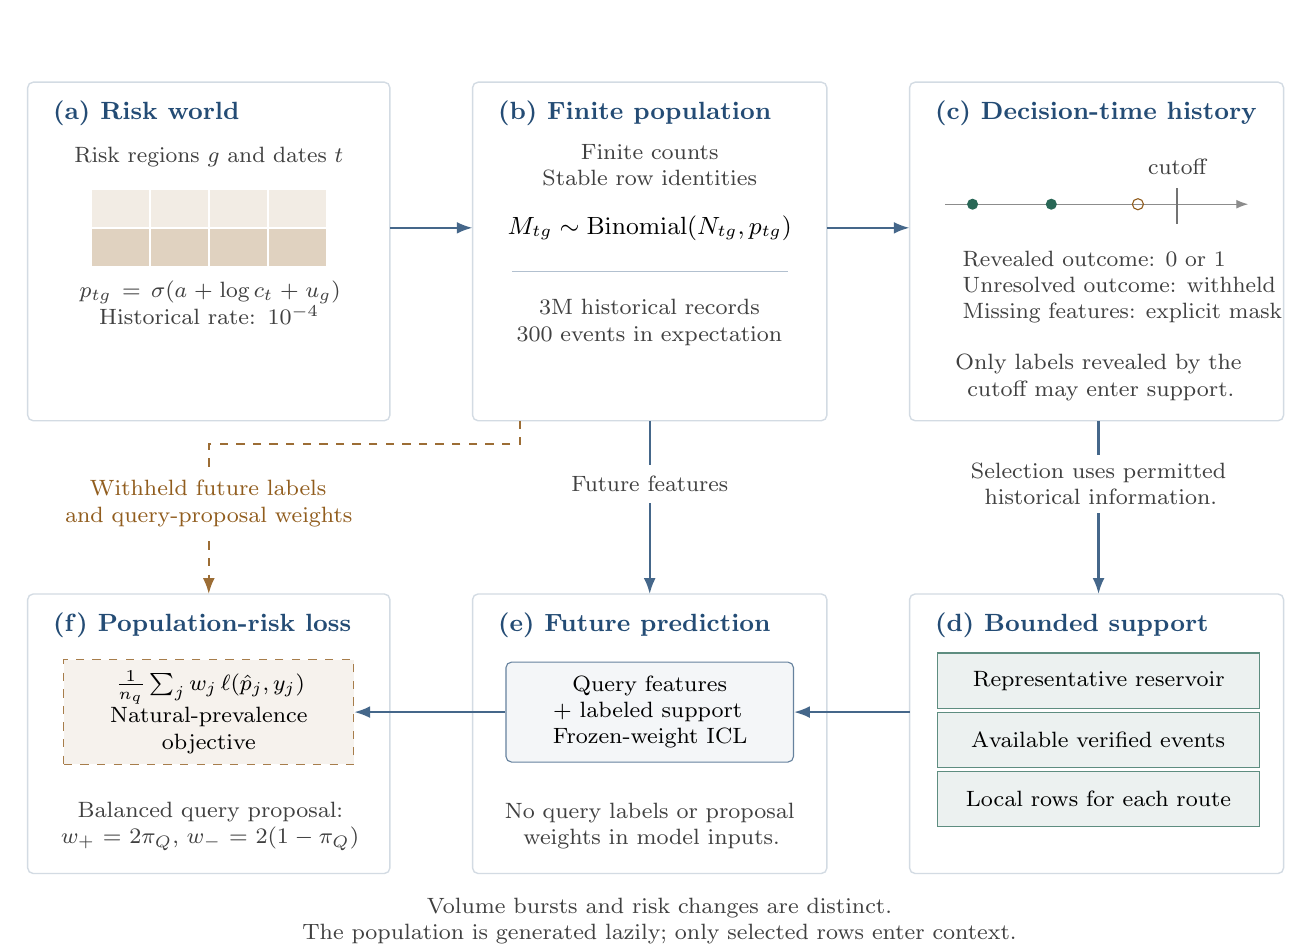
\begin{tikzpicture}[x=1cm,y=1cm,
  font=\small,
  panel/.style={draw=pfnblue!20,line width=.5pt,rounded corners=2pt,fill=white},
  title/.style={font=\small\bfseries,text=pfnblue,anchor=west},
  note/.style={font=\footnotesize,align=center,text=black!75},
  process/.style={font=\footnotesize,draw=pfnblue!70,fill=pfnblue!5,rounded corners=2pt,align=center,inner sep=5pt},
  support/.style={font=\footnotesize,draw=pfngreen!75,fill=pfngreen!9,align=center,inner sep=4pt},
  query/.style={font=\footnotesize,draw=pfnblue!70,fill=pfnblue!8,align=center,inner sep=4pt},
  hidden/.style={font=\footnotesize,draw=pfnamber!80,fill=pfnamber!8,align=center,inner sep=4pt,dashed},
  flow/.style={-{Latex[length=2mm]},draw=pfnblue!85,line width=.8pt},
  target/.style={-{Latex[length=2mm]},draw=pfnamber!90,line width=.8pt,dashed},
  reuse/.style={-{Latex[length=2mm]},draw=pfngreen!90,line width=.8pt,dashed}]

\path[use as bounding box] (0,.2) rectangle (16,-11.1);
\draw[panel] (0,0) rectangle (4.6,-4.3);
\draw[panel] (5.65,0) rectangle (10.15,-4.3);
\draw[panel] (11.2,0) rectangle (15.95,-4.3);
\node[title] at (.2,-.4) {(a) Risk world};
\node[title] at (5.85,-.4) {(b) Finite population};
\node[title] at (11.4,-.4) {(c) Decision-time history};
\node[note] at (2.3,-.95) {Risk regions $g$ and dates $t$};
\foreach \rr/\shade in {0/12,1/28}
  \foreach \cc in {0,1,2,3}
    \draw[draw=white,line width=.8pt,fill=pfnamber!\shade]
      (.8+.75*\cc,-1.35-.5*\rr) rectangle ++(.75,-.5);
\node[note,text width=4cm] at (2.3,-2.8)
  {$p_{tg}=\sigma(a+\log c_t+u_g)$\\Historical rate: $10^{-4}$};
\draw[flow] (4.6,-1.85)--(5.65,-1.85);
\node[note,text width=4cm] at (7.9,-1.05)
  {Finite counts\\Stable row identities};
\node[font=\small,align=center] at (7.9,-1.85)
  {$M_{tg}\sim\operatorname{Binomial}(N_{tg},p_{tg})$};
\draw[pfnblue!35] (6.15,-2.4)--(9.65,-2.4);
\node[note,text width=3.9cm] at (7.9,-3.05)
  {3M historical records\\300 events in expectation};
\draw[flow] (10.15,-1.85)--(11.2,-1.85);
\draw[-{Latex[length=1.5mm]},black!45] (11.65,-1.55)--(15.5,-1.55);
\draw[black!55,line width=.8pt] (14.6,-1.35)--(14.6,-1.8);
\node[note,anchor=south] at (14.6,-1.3) {cutoff};
\fill[pfngreen] (12,-1.55) circle (2pt);
\fill[pfngreen] (13,-1.55) circle (2pt);
\draw[pfnamber] (14.1,-1.55) circle (2pt);
\node[note,align=left,anchor=west] at (11.75,-2.6)
  {Revealed outcome: $0$ or $1$\\Unresolved outcome: withheld\\Missing features: explicit mask};
\node[note,text width=4.1cm] at (13.6,-3.75)
  {Only labels revealed by the cutoff may enter support.};
\draw[panel] (11.2,-6.5) rectangle (15.95,-10.05);
\node[title] at (11.4,-6.9) {(d) Bounded support};
\node[support,text width=3.8cm,minimum height=7mm] at (13.6,-7.6)
  {Representative reservoir};
\node[support,text width=3.8cm,minimum height=7mm] at (13.6,-8.35)
  {Available verified events};
\node[support,text width=3.8cm,minimum height=7mm] at (13.6,-9.1)
  {Local rows for each route};
\draw[flow] (13.6,-4.3)--(13.6,-6.5);
\node[note,fill=white,inner sep=3pt,text width=3.7cm] at (13.6,-5.1)
  {Selection uses permitted historical information.};
\draw[panel] (5.65,-6.5) rectangle (10.15,-10.05);
\node[title] at (5.85,-6.9) {(e) Future prediction};
\node[process,text width=3.3cm,minimum height=12mm] (predict) at (7.9,-8)
  {Query features\\+ labeled support\\Frozen-weight ICL};
\node[note,text width=3.9cm] at (7.9,-9.45)
  {No query labels or proposal weights in model inputs.};
\draw[flow] (11.2,-8)--(predict.east);
\draw[flow] (7.9,-4.3)--(7.9,-6.5);
\node[note,fill=white,inner sep=4pt] at (7.9,-5.1) {Future features};
\draw[panel] (0,-6.5) rectangle (4.6,-10.05);
\node[title] at (.2,-6.9) {(f) Population-risk loss};
\node[hidden,text width=3.4cm,minimum height=12mm] (loss) at (2.3,-8)
  {$\frac{1}{n_q}\sum_j w_j\,\ell(\hat p_j,y_j)$\\Natural-prevalence objective};
\node[note,text width=4cm] at (2.3,-9.45)
  {Balanced query proposal:\\$w_+=2\pi_Q$, $w_-=2(1-\pi_Q)$};
\draw[flow] (predict.west)--(loss.east);
\draw[target] (6.25,-4.3)--(6.25,-4.6)--(2.3,-4.6)--(2.3,-6.5);
\node[note,text=pfnamber,fill=white,inner sep=3pt,text width=4cm] at (2.3,-5.35)
  {Withheld future labels\\and query-proposal weights};
\node[note,text width=15cm] at (8,-10.65)
  {Volume bursts and risk changes are distinct.\\The population is generated lazily; only selected rows enter context.};

\end{tikzpicture}
\caption{Finite-population finance prior. Historical labels enter the context only after their reveal times. Future labels determine the training-query proposal and its importance weights, but are withheld from the predictor. Counts and deterministic row identities represent the population lazily, allowing a large history to supply a bounded context. Solid arrows show data and prediction flow; the dashed arrow carries training targets.}
\label{fig:finance-generation}
\end{figure}



The selected \texttt{risk\_partition} candidate fixes historical target prevalence at $\pi=10^{-4}$. It replaces the legacy assumption that class labels select separated Gaussian motifs. The number of binary risk factors $d$ is uniform on $\{2,3,4,5\}$. Their independent Bernoulli probabilities follow $\operatorname{Beta}(2,2)$ clipped to $[.05,.95]$, whose product gives weights $w_g$ for the $2^d$ cells. Each day allocates finite records as $N_{tg}\sim\operatorname{Multinomial}(N_t,w)$.

Sparse signed main effects and a signed pair interaction define cell risk scores. These are centered and normalized under $w$, then multiplied by strength $U(.5,4)$. The default gives equal weight to main and interaction components; rotation is applied with probability one-half.

Cell and campaign effects jointly determine event probability:
\[
 p_{tg}=\operatorname{sigmoid}(a+\log c_t+u_g),\qquad
 \sum_{t\in\mathrm{history},g}N_{tg}p_{tg}/N_H=\pi.
\]
Bisection solves the intercept equation using realized covariate counts. Independent draws $M_{tg}\sim\operatorname{Binomial}(N_{tg},p_{tg})$ then set the event counts. The calibration conditions expected prevalence on features, without conditioning on observed outcomes: actual counts vary and can be zero. There is no minimum positive quota or rejection for insufficient learnability. Existing future drift can change later prevalence. Multiclass diagnostics divide events using a cell-specific Dirichlet mode vector.

Within each cell, rows receive signed half-normal risk coordinates and Gaussian nuisance coordinates, followed by the specified rotation and observation process. Given day and cell, non-H covariates are independent of the realized outcome. H is drawn afterward from its class-conditional probabilities and removed before both retrieval and model input for the candidate.

Finite-ID sampling, reveal-time rules, the natural reservoir, enriched support and importance-weighted future objective remain as specified above. Additional \texttt{feature\_view} settings expose H alone or the full feature set; \texttt{positive\_h\_probability} supports a generatively nondiscriminative H control.

Changing the view or world normalization preserves \texttt{population\_id} and query draws, whereas changing generative H probabilities defines a different population law. Missingness, reveal timing and selection can still carry information. The resulting finite threshold-risk model includes overlap and conditional interactions, but not a general continuous hazard or entity-specific attack mechanism. Its oracle risk envelope is recorded across worlds rather than used to retain only worlds with attractive AP.

Unit normalization preserves the proper population objective. Section~\ref{sec:specialist} explains the use of this objective in a specialist; it does not assume that an unweighted mixture with standard tasks is safe.

\section{The shared dense in-context model}
\label{sec:icl-blueprint}

The selected 317,116,304-parameter model uses a common dense backbone for classification and regression. Its two stages of cell processing produce one representation per row, which a 24-layer transformer then interprets in the context of labeled support examples. Numerical, categorical, temporal and customer features share this table interface. The choice of a common backbone allows these tasks to use the same learned inference procedure while retaining task-specific outputs. The specification distinguishes this selected configuration from the original 315,021,456-parameter ICL-315 control; architecture comparisons keep the prior fixed so that their effects can be attributed to the predictor.

The description follows the information available to the model: support-fitted cell representations, column and row processing, contextual prediction, and the additional inputs used for finance. Section~\ref{sec:latency-moe} then considers how the same computation can reuse support state and how historical evidence is selected when it is too large to enter the transformer in full. The implemented dense path provides the reference for the optional architecture experiments discussed there.


\subsection{Architecture overview}
\label{sec:model-overview}

A query prediction requires both a description of the record and evidence about the task. The codec first distinguishes numerical values, category identities and missing observations. The cell frontend then learns interactions among a record's features, conditioned on summaries of the support table. Finally, the row transformer relates the query representation to labeled support rows. Figure~\ref{fig:model-overview} shows these three parts and the direction in which information passes between them.

Column processing supplies a learned description of each feature's support values, while row processing combines the features that belong to one record. Eight learned summary tokens carry the result into the larger row transformer. These tokens represent a row collectively; none is defined as a selected raw column or a selected training example. This compression makes the wide contextual transformer affordable, but it also creates a bottleneck. Tasks whose predictions depend on fine feature detail therefore provide a necessary test of what the summaries retain.

\begin{figure}[htbp]
\centering
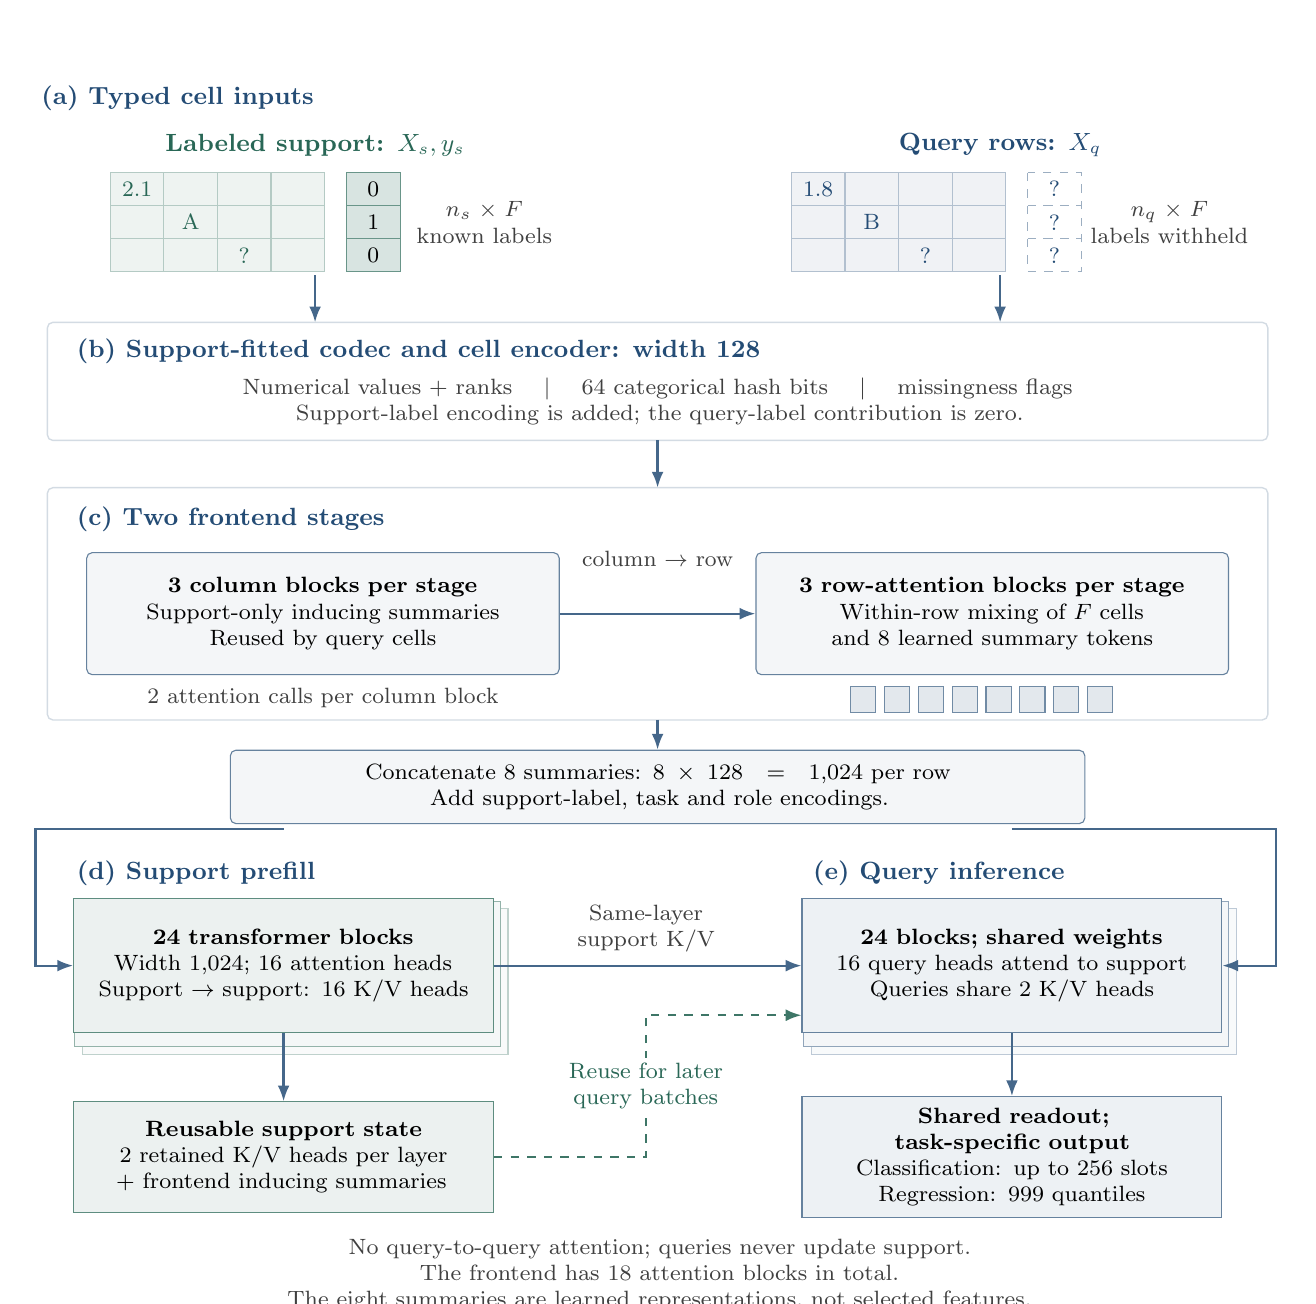
\begin{tikzpicture}[x=1cm,y=1cm,
  font=\small,
  panel/.style={draw=pfnblue!20,line width=.5pt,rounded corners=2pt,fill=white},
  title/.style={font=\small\bfseries,text=pfnblue,anchor=west},
  note/.style={font=\footnotesize,align=center,text=black!75},
  process/.style={font=\footnotesize,draw=pfnblue!70,fill=pfnblue!5,rounded corners=2pt,align=center,inner sep=5pt},
  support/.style={font=\footnotesize,draw=pfngreen!75,fill=pfngreen!9,align=center,inner sep=4pt},
  query/.style={font=\footnotesize,draw=pfnblue!70,fill=pfnblue!8,align=center,inner sep=4pt},
  hidden/.style={font=\footnotesize,draw=pfnamber!80,fill=pfnamber!8,align=center,inner sep=4pt,dashed},
  flow/.style={-{Latex[length=2mm]},draw=pfnblue!85,line width=.8pt},
  target/.style={-{Latex[length=2mm]},draw=pfnamber!90,line width=.8pt,dashed},
  reuse/.style={-{Latex[length=2mm]},draw=pfngreen!90,line width=.8pt,dashed}]

\path[use as bounding box] (0,.2) rectangle (16,-15.65);
\node[title] at (.05,-.2) {(a) Typed cell inputs};
\node[font=\small\bfseries,text=pfngreen] at (3.65,-.8) {Labeled support: $X_s,y_s$};
\node[font=\small\bfseries,text=pfnblue] at (12.35,-.8) {Query rows: $X_q$};
\foreach \rr in {0,1,2}
  \foreach \cc in {0,1,2,3}{
    \draw[draw=pfngreen!35,fill=pfngreen!8] (1.05+.68*\cc,-1.15-.42*\rr) rectangle ++(.68,-.42);
    \draw[draw=pfnblue!35,fill=pfnblue!7] (9.7+.68*\cc,-1.15-.42*\rr) rectangle ++(.68,-.42);
  }
\foreach \rr/\val in {0/0,1/1,2/0}{
  \draw[draw=pfngreen!70,fill=pfngreen!18] (4.05,-1.15-.42*\rr) rectangle ++(.68,-.42);
  \node[font=\footnotesize] at (4.39,-1.36-.42*\rr) {$\val$};
  \draw[draw=pfnblue!45,dashed] (12.7,-1.15-.42*\rr) rectangle ++(.68,-.42);
  \node[font=\footnotesize,text=pfnblue] at (13.04,-1.36-.42*\rr) {?};
}
\node[note,text width=2cm] at (5.8,-1.78) {$n_s\times F$\\known labels};
\node[note,text width=2cm] at (14.5,-1.78) {$n_q\times F$\\labels withheld};
\node[font=\footnotesize,text=pfngreen] at (1.39,-1.36) {2.1};
\node[font=\footnotesize,text=pfngreen] at (2.07,-1.78) {A};
\node[font=\footnotesize,text=pfngreen] at (2.75,-2.2) {?};
\node[font=\footnotesize,text=pfnblue] at (10.04,-1.36) {1.8};
\node[font=\footnotesize,text=pfnblue] at (10.72,-1.78) {B};
\node[font=\footnotesize,text=pfnblue] at (11.4,-2.2) {?};
\draw[panel] (.25,-3.05) rectangle (15.75,-4.55);
\node[title] at (.5,-3.42) {(b) Support-fitted codec and cell encoder: width 128};
\node[note,text width=14.5cm] at (8,-4.05)
  {Numerical values + ranks \quad $\vert$ \quad 64 categorical hash bits \quad $\vert$ \quad missingness flags\\Support-label encoding is added; the query-label contribution is zero.};
\draw[flow] (3.65,-2.45)--(3.65,-3.05);
\draw[flow] (12.35,-2.45)--(12.35,-3.05);
\draw[panel] (.25,-5.15) rectangle (15.75,-8.1);
\node[title] at (.5,-5.55) {(c) Two frontend stages};
\node[process,text width=5.65cm,minimum height=15.5mm] (column) at (3.75,-6.75)
  {\textbf{3 column blocks per stage}\\Support-only inducing summaries\\Reused by query cells};
\node[process,text width=5.65cm,minimum height=15.5mm] (row) at (12.25,-6.75)
  {\textbf{3 row-attention blocks per stage}\\Within-row mixing of $F$ cells\\and 8 learned summary tokens};
\draw[flow] (8,-4.55)--(8,-5.15);
\draw[flow] (column.east)--(row.west);
\node[note] at (8,-6.05) {column $\rightarrow$ row};
\node[note] at (3.75,-7.82) {2 attention calls per column block};
\foreach \cc in {0,1,2,3,4,5,6,7}
  \draw[draw=pfnblue!65,fill=pfnblue!13] (10.45+.43*\cc,-7.68) rectangle ++(.32,-.32);
\node[process,text width=10.5cm,minimum height=9mm] (compress) at (8,-8.95)
  {Concatenate 8 summaries: $8\times128=1{,}024$ per row\\Add support-label, task and role encodings.};
\draw[flow] (8,-8.1)--(compress.north);
\node[title] at (.5,-10.05) {(d) Support prefill};
\node[title] at (9.85,-10.05) {(e) Query inference};
\draw[draw=pfngreen!30,fill=pfngreen!3] (.7,-10.5) rectangle (6.1,-12.35);
\draw[draw=pfngreen!50,fill=pfngreen!5] (.6,-10.4) rectangle (6,-12.25);
\node[support,text width=5.05cm,minimum height=17mm] (strunk) at (3.25,-11.22)
  {\textbf{24 transformer blocks}\\Width 1,024; 16 attention heads\\Support $\rightarrow$ support: 16 K/V heads};
\draw[draw=pfnblue!30,fill=pfnblue!3] (9.95,-10.5) rectangle (15.35,-12.35);
\draw[draw=pfnblue!50,fill=pfnblue!5] (9.85,-10.4) rectangle (15.25,-12.25);
\node[query,text width=5.05cm,minimum height=17mm] (qtrunk) at (12.5,-11.22)
  {\textbf{24 blocks; shared weights}\\16 query heads attend to support\\Queries share 2 K/V heads};
\draw[flow] (3.25,-9.48)--(.1,-9.48)--(.1,-11.22)--(strunk.west);
\draw[flow] (12.5,-9.48)--(15.85,-9.48)--(15.85,-11.22)--(qtrunk.east);
\draw[flow] (strunk.east)--(qtrunk.west);
\node[note,fill=white,inner sep=2pt,text width=2.65cm] at (7.85,-10.75)
  {Same-layer\\support K/V};
\node[support,text width=5.05cm,minimum height=14mm] (cache) at (3.25,-13.65)
  {\textbf{Reusable support state}\\2 retained K/V heads per layer\\+ frontend inducing summaries};
\node[query,text width=5.05cm,minimum height=14mm] (head) at (12.5,-13.65)
  {\textbf{Shared readout; task-specific output}\\Classification: up to 256 slots\\Regression: 999 quantiles};
\draw[flow] (strunk.south)--(cache.north);
\draw[flow] (qtrunk.south)--(head.north);
\draw[reuse] (cache.east)--(7.85,-13.65)--(7.85,-11.85)--(qtrunk.west |- 7.85,-11.85);
\node[note,text=pfngreen,fill=white,inner sep=2pt,text width=2.2cm] at (7.85,-12.75)
  {Reuse for later\\query batches};
\node[note,text width=14.7cm] at (8,-15.15)
  {No query-to-query attention; queries never update support.\\The frontend has 18 attention blocks in total.\\The eight summaries are learned representations, not selected features.};

\end{tikzpicture}
\caption{The proposed 317,116,304-parameter model. Support and query paths share weights. Each column summary block contains two attention calls, giving 18 frontend attention blocks in total. The query path shares two KV heads, reducing retained cache storage; support prefill uses all 16 heads. Queries neither attend to one another nor update support states. The optional severity head is omitted here and is not trained by the standard and binary-fraud runs. Matrices and layer stacks are schematic; dimensions are stated explicitly.}
\label{fig:model-overview}
\end{figure}

The support/query boundary also makes repeated prediction economical. For fixed support and weights, preparing the support builds the codec and caches once; subsequent query chunks reuse them. A query's prediction is mathematically independent of the other query rows, with implementation comparisons allowing numerical tolerance. This reuse separates context-setup cost from repeated query cost, although every query still pays for attention to its support set. Changes to support, weights or relevant preprocessing state require the affected cache to be rebuilt.

The computation in the figure applies to one ragged episode. The current API processes episodes separately, and the trainer accumulates their losses into a logical global batch; it does not pack unrelated tasks into a single padded attention tensor. The dimensions, residual operations and visibility masks below specify that episode-level computation.

\subsection{Input codec and tensor representation}
\label{sec:codec}

For an episode, let $n_s$ and $n_q$ denote the support and query sizes, $N=n_s+n_q$ their total, and $F$ the actual feature count. The batch dimension is omitted below. The forward signature contains $X_s$, $y_s$, $X_q$, feature-type masks, task type and the legal class vocabulary. Query targets are held in a separate loss-only object and are never read by the model.

The vocabulary is part of the task definition rather than an inference from scored outcomes. Synthetic training samples a declared vocabulary before outcomes; deployment without an independently declared vocabulary uses the support/training-fold vocabulary. A query class outside that vocabulary is reported as unsupported and remains in evaluation. Its occurrence changes neither the label mapping nor the acceptance rule. The native head accommodates 256 classes.

Numerical normalization is fitted to finite support values so that each query is interpreted on the same scale as its evidence. For each feature, the center $m$ is their median and $\mathrm{MAD}=\mathrm{median}(|x-m|)$ determines the preferred scale $s=1.4826\mathrm{MAD}$. When MAD is at most $10^{-12}$, the population standard deviation replaces it; when that too is at most $10^{-12}$, the scale is one. A final floor of $10^{-3}$ prevents $s$ from becoming arbitrarily small. Empty finite support uses $m=0,s=1$, and even-length medians average the two middle values. The standardized value $z=(x-m)/s$ is computed in a sufficiently wide accumulator, with separate indicators retaining information about clipping.

The numerical representation preserves several views of a value because magnitude, order and exceptional observations can carry different predictive information. Its eight base channels are $\operatorname{clip}(z,-100,100)$, $\operatorname{sign}(z)\log(1+\min(|z|,10^6))$, support midrank, missingness, positive infinity, negative infinity, $z<-100$, and $z>100$. With $n_f$ finite support values, midrank is $(\#\{x_s<x\}+\tfrac12\#\{x_s=x\}+\tfrac12)/(n_f+1)$. Nonfinite values and empty-reference cases receive rank $1/2$, zero value payloads and the corresponding explicit flags.

The encoder supplements these channels with 32 learned sine/cosine frequency pairs of clipped $z$ and eight fixed pairs at rank frequencies $1,\ldots,8$, producing 88 channels. The learned positive frequencies begin logarithmically spaced from 0.01 to 10. Optimization acts on their logarithms, while the forward pass clips the resulting frequencies to $[10^{-4},100]$. All Fourier arguments include $2\pi$.

Missingness is an observation in this representation, rather than a request to fill in a complete feature matrix. A numerical NaN has a finite placeholder payload and an explicit missingness flag; numerical location, scale and rank references exclude missing entries. A missing category is likewise distinct from an observed category that was absent from support. Support target labels remain required; this feature encoding does not manufacture missing labels.

The selected categorical encoder represents a SHA-256 prefix by 64 signed bits. Support frequency, an unknown-category indicator and a missing-value indicator bring the input to each categorical projection to 67 coordinates. The discrete bits are exactly representable in BF16, avoiding the need to distinguish identities through small differences in a smooth scalar code. Typed keys, column namespaces and recoding seeds define the hash; support collision checks leave query transformations fixed. The projection count is 384 parameters smaller than in the scalar-Fourier control.

Under an ideal random hash, a million keys have collision probability approximately $2.7\cdot10^{-8}$ before the observed-support check. In the precision probe described below, the audited aliasing pair separates under all six tested hash-bit initializations. That result establishes separation at initialization for this pair. Whether the trained projection continues to retain useful category information remains an empirical question.

The retained scalar-Fourier control makes the representational difference explicit. Its categorical vector starts with four channels: a deterministic random code in $[-1,1)$, support relative frequency, an unseen-in-support flag and a missing flag. Adding 32 learned Fourier pairs of the code gives 68 channels. The scalar code uses the first 53 SHA256 bits of a length-prefixed serialization of encoding seed, stable feature identity and type-tagged category value. It is a random identity representation rather than a language embedding.

Collision handling is restricted to observed support keys. A collision redraws the encoding stream up to eight times, after which the episode fails explicitly. The current codec does not detect or log query-code collisions; query values cannot change the encoding seed, support codes or task acceptance. Unseen keys can therefore still have finite hash collisions. The same dictionary/hash rule applies to support and query values, including unseen queries. Missing categories receive zero payload/Fourier features together with their missing flag.

The reference codec computes codes, normalization/ranks, Fourier phases and trigonometric features in FP64, then casts completed vectors to FP32 before BF16 projection. An FP32 codec fast path requires independent validation. The audit includes collisions after casting on fixed inputs, because distinct source hashes alone do not establish distinct numerical representations.

The independent precision probe illustrates why the post-projection check matters. Among 50,000 categories with encoding seed zero, \texttt{category\_28838} and \texttt{category\_39200} have distinct scalar codes separated by $1.6093\times10^{-9}$. Although they pass the support hash audit, a seeded tiny cell encoder maps them to identical vectors under CPU BF16 autocast; the maximum FP32 difference is $3.58\times10^{-7}$. This reproducible counterexample concerns one encoder and one pair, rather than every trained encoder or GPU implementation. The corresponding hardware validation therefore tests identity after projection, including random recodings and held-out category counts.

After numerical or categorical encoding, a small feature grouping gives each cell access to neighboring coordinates before attention. At feature position $j$, three slot-specific, bias-free projections read positions $j$, $(j+1)\bmod F$ and $(j+3)\bmod F$ and sum their outputs into width 128. Numerical and categorical projections and frequency banks are separate for each slot. Every anchor position remains present, so the result contains $N\times F\times128$ tokens rather than $F/3$ tokens.

Each token also receives the anchor feature's learned type vector, task and support/query-role vectors, and a support-label embedding. Classification labels use a $256\times128$ lookup. Regression labels pass through a bias-free projection of standardized target, signed logarithm and clipping indicator, with raw clipping at 20 and logarithm clipping at $10^6$. Query label contributions are literal zero tensors. An affine LayerNorm with epsilon $10^{-5}$ completes the cell encoder.

\subsection{Column conditioning, row summaries and attention masks}
\label{sec:attention}

The column and row blocks separate two interactions that have different visibility requirements. Columns summarize how a feature behaves across support examples; rows combine features within one example. The frontend implements two stages, each with three column ISABs followed by three row self-attention blocks. All use width 128, eight heads of dimension 16 and SwiGLU hidden width 512. Each ISAB owns 128 learnable inducing vectors and computes, independently for each feature,
\[
 H_j=\operatorname{MAB}(I_j,Z_{s,j}),\qquad
 Z_{:,j}=\operatorname{MAB}(Z_{:,j},H_j).
\]
Sharing the inducing parameters across feature positions makes the same summarization operation available to every feature, while its induced summaries remain specific to the feature and episode. Only support rows supply keys and values to the first attention call. Missing observed cells remain valid tokens because their flags convey information. Where padding is present, only padding is masked.

Row compression is learned jointly with those feature interactions. Eight learned summary tokens are appended before the first row block, and each row block attends across the row's $F+8$ tokens. Queries and keys in row attention alone receive parameter-free rotary encoding with base 10,000, using feature positions $0,\ldots,F-1$ and summary positions $F,\ldots,F+7$. The summary tokens persist between stages: the second column stage updates the feature tokens while carrying the summaries unchanged. Concatenating the final eight summaries produces $R\in\mathbb R^{N\times1024}$. Separate width-1,024 task, role and support-label embeddings/projections are added at this boundary, using the same label channel definitions as the cell encoder.

The row transformer uses the labeled support as the task context. Its 24 untied blocks have width 1,024, 16 full attention heads of dimension 64 and SwiGLU hidden width 2,816, with no row-position encoding. In each block, a support row attends to support rows, including itself, and a query attends to support rows only. A query never supplies keys or values, even to itself; its own features remain available through the residual stream. The visibility mask is therefore
\[
 M=\begin{pmatrix}0_{n_s\times n_s}&-\infty_{n_s\times n_q}\\
 0_{n_q\times n_s}&-\infty_{n_q\times n_q}\end{pmatrix}.
\]
This boundary permits support caching and independent query chunks without query-batch transduction. Any padded or packed implementation would also have to mask support padding and isolate episodes; the current ragged API keeps episodes separate. Standard training uses nonempty support. The generic model additionally defines the empty-support case needed by the finance extension: with no legal keys, the attention branch contributes zero, leaving the residual computation and default codec statistics in place.

Attention and feature transformation use the same residual convention throughout the model. Every MAB has bias-free Q/K/V/output matrices and three SwiGLU matrices, applied in the order
\[
\begin{aligned}
 U&=Q+\mathrm{RMS}_2(\mathrm{Attn}(\mathrm{RMS}_1(Q),\mathrm{RMS}_1(KV))),\\
 O&=U+\mathrm{RMS}_4\{W_d[\mathrm{SiLU}(W_g\mathrm{RMS}_3(U))\odot W_v\mathrm{RMS}_3(U)]\}.
\end{aligned}
\]
The first RMS module normalizes both the query and key/value streams with shared parameters. Each of the four RMS modules has a learned gain, no bias and epsilon $10^{-6}$. Projected Q/K vectors receive a further per-head normalization, with separate learned head-dimension gains shared across heads. Where rotary encoding is used, this normalization precedes it.

The attention temperature controls how a fixed representation is used as the number of visible keys changes. In the legacy control, each head's $QK^\top/\sqrt{d_h}$ is multiplied by
\[\tau_h(n)=\exp\{\tanh(a_h)\operatorname{clip}[\log(\max(n,1)/1024),-\log4,\log4]\},\]
where $n$ is the legal-key count and $a_h$ is initialized at zero. The selected candidate replaces this bounded rule in support-reading inducing attention and the ICL trunk with
\[
T_h(n)=\frac{\operatorname{softplus}(a_h)}{\log 2}
        \frac{\log(\max(n,2))}{\log 1024},\qquad a_h(0)=0.
\]
The replacement starts at one for 1,024 keys and continues to increase beyond the legacy rule's 4,096-key saturation point. Fixed-size inducing summaries and row-feature attention retain the control temperature. For queries, the key count comes from the cached support, so the temperature does not depend on query chunk size. This logarithmic rule is a specified alternative; it does not reproduce all details of QASSMax.

Dropout is zero. Ordinary linear weights are initialized with standard deviation $1/\sqrt{\mathrm{fan\_in}}$, embeddings with 0.02, and output-head matrices with $0.02/\sqrt{\mathrm{fan\_in}}$. RMS gains begin at one except for the residual-output gains, which use $1/\sqrt{36}$ in the 18 frontend MABs and $1/\sqrt{48}$ in the 24 ICL blocks.

\subsection{Prediction heads and parameter accounting}
\label{sec:heads}

A final width-1,024 RMSNorm and shared bias-free $1024\to1024$ exact-GELU layer feed the task heads. The selected ordinary-regression head predicts quantiles; its resolution and loss are discussed below alongside the original density control. Classification uses 256 logits with illegal classes masked and cross-entropy on the legal outputs. During training, an episode's $K$ declared labels are independently injected into an ordered $K$-element subset sampled without replacement from all 256 slots. Masking the remaining slots permits training across the whole head even when $K$ is small. Deployment may use a deterministic mapping to the first $K$ slots. Standard query targets are the sampled outcomes, while finance queries carry the loss-only importance weights of Section~\ref{sec:finance-objective}.

The original regression control is retained because it defines a normalized density with an explicit tail model. Its projection emits 132 values: 130 bin probabilities and two tail-scale parameters. Targets use the support-only median/MAD transform and the numerical fallbacks above. The density has 128 uniform finite bins on $[-5,5]$ and two Lomax tails of shape three, with scales $0.05+\mathrm{softplus}(u)$. The left tail applies below $-5$, finite half-open bins cover $[-5,5)$, and the right tail applies at or above 5. Likelihood evaluation uses FP32. The original-unit density is $p_z((y-m)/s)/s$, including the affine Jacobian in log scores. Its point mean combines finite-bin midpoints and predicted masses with tail means $-5-s_L/2$ and $5+s_R/2$, then inverts the support affine transform. Comparisons intended to isolate the prior retain the unchanged reference head, rather than combining a prior change with this head choice.

For distance $v\geq0$ from a tail boundary, the tail density is $3s^{-1}(1+v/s)^{-4}$. Its analytic piecewise CDF supplies quantiles, and both first and second moments are finite. Thus the control supplies a normalized predictive density without fitting bin edges to queries. Realized finance losses require an additional mass at zero, specified in Section~\ref{sec:finance-head}.

An integer-valued target requires a probability mass function if it is to be evaluated as a discrete outcome. In a separately declared discrete track, the CDF can assign mass to $[k-1/2,k+1/2)$, conditioned on the declared integer support. For nonnegative counts, normalization uses the mass above $-1/2$, and negative targets fail schema validation. Count means and quantiles then come from this PMF with a certified tail bound, or from an explicit count head. A continuous density value is not a count probability, and the continuous mean above is not the exact expectation after rounding. The initial generic-regression comparison may instead use continuous scoring and point metrics, as long as that choice is explicit and common to all priors.

For reproducible accounting, the original dense control can be assembled from the parameter count of a MAB with width $d$, hidden width $h$, head dimension $d_h$ and $H$ heads:
$4d^2+3dh+4d+2d_h+H$ parameters. The 18 frontend MABs therefore contain 4,728,528 parameters, and the ICL trunk contains 308,383,104. The remaining components are inducing vectors, 98,304; summary tokens, 1,024; cell projections, 59,904; Fourier frequencies, 192; type/task/role vectors, 4,864; class-label lookups, 294,912; regression-label projections, 3,456; input LayerNorm, 256; head matrices, 1,445,888; and final RMSNorm, 1,024. These sum to the control's exact total of \textbf{315,021,456}. Every component is recorded in the paired JSON, and a pre-launch assertion checks the implementation against its specified count.

The mask gives exact mathematical invariance to support-row permutation and independence from other query rows, with numerical tolerance in implementation checks. Other symmetries are learned only approximately. Grouping and rotary positions make feature permutation consequential; chosen hash codes can make category renaming consequential; and learned lookup/output matrices can make class relabeling consequential. The model is consequently \emph{not} exactly invariant to these transformations. Augmentation encourages the desired behavior without proving it. A permutation-equivariant set encoder would be a distinct ablation.

\paragraph{Regression resolution motivates the selected quantile head.}
The regression-head choice follows from a mismatch between finite-bin likelihood resolution and point error. Targets $z=0.005$ and $z=0.070$ occupy the same finite bin, so their NLL and all 132 output gradients are exactly identical. Normalization of the density does not remove this blindness. In a noiseless constant task, the support codec gives center $c$ and scale one, placing $z=0$ at the left boundary of $[0,0.078125)$. Population-optimal NLL concentrates mass in that bin, but its original-unit mean is $c+0.0390625$. The resulting point bias remains even with perfect likelihood optimization and cannot be corrected by adding backbone parameters.

The implemented alternatives address this resolution issue in different ways. The finer-histogram candidate uses 1,025 equal-width bins on $[-5,5]$ together with the same two tails and scales, giving 1,029 outputs. Its central bin has midpoint zero, and its width $10/1025$ is about eight times finer. At width 1,024 this adds 918,528 output weights. It removes the constant-target example and reduces the range of indistinguishable targets, while retaining some within-bin blindness.

The selected ordinary-regression head instead follows the reference 999-quantile pinball approach. TabICLv2 found it effective for RMSE, whereas LimiX-2 uses a much finer histogram \cite{tabicl2,limix2}. The head emits 999 unconstrained values at levels $k/1000$, $k=1,\ldots,999$, and minimizes their mean pinball score in support-standardized units. Reported quantiles are sorted, and the point readout averages the finite grid. These outputs support quantile and point-prediction evaluation but do not define a density likelihood.

Both the finer-histogram and 999-quantile alternatives are implemented, with the 132-output head retained as a control. An auxiliary mean readout trained by a proper squared-error objective could separate point accuracy from likelihood resolution, but remains unimplemented. A finite quantile grid also leaves a tail limitation: if $P(Y=10^6)=10^{-4}$ and otherwise $Y=0$, all of its population quantiles are zero even though the mean is 100. Accurate values on the grid therefore do not guarantee an accurate extreme-tail mean.

\paragraph{Learned head-resolution check.} A small CPU experiment tested whether the analytical resolution defect persists after optimization. Identical two-input MLPs were fitted to noiseless conditional targets $.005$ and $.070$, with an independent nuisance variable. Across three seeds, 1,000 Adam steps, 64 training rows and 512 held-out rows, the 128-bin head achieved RMSE $.032537$--$.032538$, the 1,025-bin head $.0035745$--$.0035752$, and the 999-quantile head $.0000409$--$.0002501$. The record in \path{research/results/learned_regression_head_probe.json} retains every seed. The old head's defect therefore survives actual training in this example, while both alternatives resolve the distinction more accurately. The experiment concerns head resolution in a small supervised problem; it does not measure full-model transfer or establish an ordering that holds for every regression distribution.

\subsection{Finance metadata and the realized-loss readout}
\label{sec:finance-head}

A finance context combines three sources of evidence. The representative reservoir $R$ describes the labeled pool, the capped eventful sample $P$ retains rare outcomes, and route-specific local rows $L_c$ supply nearby examples. Their deduplicated union is $C_c$. Here $N$ denotes the number of eligible labeled historical records, $M$ their eventful count and $M_R$ the eventful count in $R$; this historical $N$ is not the row count of a model forward pass. Section~\ref{sec:finance-context} gives the selection procedure. All these counts concern historical evidence available to the learner, not hidden future prevalence.

The model needs to know how a selected context relates to its available history. Ordinary feature standardization would remove quantities that are constant across that context, so they enter through a separate metadata vector. Its 14 coordinates are
\begin{align*}
&\log(1+N),\ \log(1+M),\ \log(1+|R|),\ \log(1+|P|),\ \log(1+|L_c|),\\
&\log(1+|C_c|),\ \log(1+M_R),\ \log(|R|/N),\ \log(|P|/M),\ \ind\{M=0\},\\
&\mathrm{reference\ kind},\ \operatorname{clip}(\operatorname{logit}\pi_{\rm ref},-40,40)/20,\ \log(1+|G|),\ \log(1+N_{\rm ref}),
\end{align*}
where $G$ is the searched candidate pool and $N_{\rm ref}$ is the size of a representative adjudicated reference cohort, or zero when no such cohort is available. Including cohort size distinguishes references that estimate the same event rate with different uncertainty. Undefined log fractions and absent reference log odds are encoded as zero.

Reference kind specifies what the rate can legitimately describe. It is zero when unavailable, one for an independent past complete cohort, and two only when the entire eligible support pool is completely adjudicated. Kind two uses $(M+.5)/(N+1)$; kind one applies the same smoothing to the separate representative reference counts. If newer selectively reviewed labels supplement an older complete cohort, the reference remains kind one. Full-amount regression sets the positive-count/fraction/absence and reference coordinates to zero, including reference cohort size. Its remaining pool-size coordinates describe the uniform and local samples.

Context metadata enters at both levels of representation so that it can affect feature interpretation and subsequent task inference. A bias-free $14\to128\to1152$ GELU MLP produces an early 128-dimensional addition and a late 1,024-dimensional addition. Separate bias-free $3\to128$ and $3\to1024$ maps encode the source-membership bits; query membership is $000$. The early additions enter row-associated cell representations before the frontend, and the late additions enter before the ICL trunk.

The first metadata matrix is initialized with standard deviation $1/\sqrt{14}$; the second matrix and the source projections begin at zero. AdamW optimizes all of these parameters. Their contribution to the model count is
\[
14(128)+128(1152)+3(128)+3(1024)=152{,}704,
\]
which brings the original control to 315,174,160 parameters before the zero-atom readout. The additional bias-free $1024\to1$ projection gives the finance-capable legacy control \textbf{315,175,184 parameters}. Substituting the selected quantile head and adding the separate finer hurdle head gives the 317,116,304 total in Section~\ref{sec:main-candidate}.

For standard episodes, metadata and source vectors are zero, making the additive finance path exactly zero. That property isolates the direct input contribution but does not freeze the backbone: shared weights could still change under joint training. Benchmark regression testing remains necessary for any sharing experiment.

When a representative reference is available, the finance classifier predicts a residual relative to its class frequencies. Binary finance adds $(\log(1-\pi_{\rm ref}),\log\pi_{\rm ref})$ to the two residual logits. Multiclass finance uses log offsets from the reference cohort's Dirichlet$(.5)$-smoothed class frequencies, aligned with the declared class permutation. Its scalar event-rate metadata separately uses Jeffreys smoothing of legitimate versus any-fraud counts, so these two declared estimates need not be numerically identical. Logs and likelihoods are computed in FP32.

Without a reference, the offset is zero and the loss normalization in Section~\ref{sec:finance-objective} is one. The zero offset records absent reference information; it is not a prevalence estimate of 50\%. Continuation retains the shared classification head. Initializing a separate residual head at zero would be an isolated experiment, rather than a reason to reset a trained shared head. Regression uses no class-logit offset.


\paragraph{Exact zero mass for realized losses.} Realized loss combines a discrete outcome---no loss---with positive severity, so a purely continuous density assigns the wrong type of probability to zero. Let the ordinary standardized density be $f(z)$ with CDF $F(z)$, support-fitted transform $z=(y-m)/s$ and zero boundary $z_0=-m/s$. A scalar readout defines $p_0=\sigma(a)$ as the mass at exactly zero. Its learned projection starts at zero. When metadata supplies a valid event-rate reference, the readout receives $-\operatorname{logit}(\pi_{\rm ref})$ before the sigmoid; otherwise the addition is zero. Thus an admissible rare-event reference sets the initial atom rather than forcing training to start from a 50\% event rate. With $Z=1-F(z_0)$, the mixed distribution is
\[
P(Y=0)=p_0,\qquad p(y>0)=\frac{(1-p_0)f((y-m)/s)}{sZ}.
\]
The corresponding loss is $-\log p_0$ for zero targets and $-\log(1-p_0)-\log f(z)+\log s+\log Z$ for positive targets. Negative realized losses are outside the target schema and fail validation. Survival mass is evaluated directly from component survival probabilities in log space, avoiding the loss of precision that can arise from subtracting a rounded CDF from one.

The predictive mean is $(1-p_0)[m+s\,E(Z_{\rm base}\mid Z_{\rm base}>z_0)]$, computed from truncated finite-bin and Lomax first moments. The atom removes the zero-bin midpoint bias of the ordinary histogram: with $m=0,s=1$, putting all mass in $[0,.078125)$ would otherwise predict $.0390625$ for an identically zero target. Density normalization, zero probability, positive-tail moments and gradients are therefore checked before training. The declared target schema determines whether the likelihood is hurdle or continuous; the choice does not depend on whether zeros happen to occur in a particular support sample.

The metadata describes selection without purporting to undo it by itself. Source fractions are not inverse inclusion probabilities for the union, because local selection depends on the reservoir-fitted codec and centers, while deduplication couples the sources. Likewise, a flag for selective review does not identify population prevalence when the review process is unknown. Until representative adjudicated outcomes become available, useful probability estimates in that setting depend on assumptions learned from the prior. Results under incomplete adjudication are consequently reported separately from empirically verified population calibration.


\paragraph{Candidate severity scaling and count.} Rare-event sampling creates a second resolution problem even with many histogram bins. At prevalence $10^{-4}$, a natural 512-row reservoir is often all zero. Fitting the target transform to that reservoir can then place most positive severities in one tail. The candidate's \texttt{positive\_support} option instead fits the hurdle target affine transform to observed positive support outcomes, using the original permitted-reservoir fallback if none are available. Feature scaling continues to use the reservoir. This change preserves the density's affine Jacobian and positive truncation, and query outcomes never enter the fit. It corrects the scale problem without establishing that the tail shape is adequate for company losses.

With hash bits, quantile999 and a separate 1,025-bin hurdle density, the complete finance-capable model contains \textbf{317,116,304 parameters}. The finer-histogram-only candidate contains 316,093,328. Neither query grouping nor the target-scaling option introduces parameters.

\section{Context selection, caching and architecture experiments}
\label{sec:latency-moe}

The deployment objective is GPU batch prediction, for which both the preparation of a context and its repeated use matter. The implemented dense model reuses exact support caches. Financial histories also use a bounded selection policy, because a history of several million rows cannot be passed directly to dense attention as one context. These two mechanisms define the current inference paths. Feature feedback, MoE and a general local/global attention graph remain research challengers, each requiring its own quality and runtime measurements.

The experiments distinguish work that preserves the predictor from changes that may discard evidence or alter its capacity. Correct caching and chunking establish the first reference; profiling then identifies the costs that justify an approximation or additional conditional capacity. Section~\ref{sec:latency-evaluation} collects the timing and accuracy protocol used to compare these choices.

\subsection{Dense context cost and exact support caches}

To separate reusable work from work paid on each prediction request, write $n=n_s$, $q=n_q$, trunk width $d=1024$ and depth $L=24$. Batch prediction time is decomposed as
\[
T_{\rm batch}=T_{\rm codec}+T_{\rm transfers}+T_{\rm support\ prefill}+T_{\rm query\ batch}+T_{\rm output}.
\]
Model loading and kernel compilation are reported separately as startup costs. A cached support table avoids another prefill, but the first request on a new dataset still includes that work. This distinction is especially relevant to benchmark evaluation and offline batch jobs, where fewer requests may share a context than in an online service.

The support prefill grows rapidly because it contextualizes support rows with one another. The dense trunk's attention products require approximately
\[
4Ld(n^2+nq)
\]
forward FLOPs, counting a multiply--add as two operations. Projections, FFNs, normalization and the frontend add to this count. The support term is quadratic, while cached query attention is linear in both $n$ and $q$. Doubling context therefore quadruples the \emph{support-attention component} and doubles the \emph{cached-query-attention component}; the effect on total wall time depends on the other work. The frontend itself costs roughly $O(FnI d_c+nF^2d_c)$ per stage, with $I=128,d_c=128$, so wide tables can remain frontend-bound even when row attention is efficient.

Exact cache reuse follows from the visibility mask. After support states are computed, the cache retains each column ISAB's support-induced summaries or their projected K/V, the fitted preprocessing state, and each trunk layer's projected support K/V. A query then uses these objects, its own features and the frozen weights. Induction over layers establishes that another query cannot affect its prediction. Cached/uncached and chunk-invariance tests verify that the implementation realizes this architectural property within declared numerical tolerances.

The full-head control provides a useful memory baseline. Its BF16 trunk K/V occupy $2Lnd\times2=98{,}304n$ bytes per estimator: 0.75\,GiB at 8,192 support rows, 3\,GiB at 32,768 and 6\,GiB at 65,536. The six frontend ISABs additionally retain projected inducing K/V of size $6F\cdot128\cdot2\cdot128\cdot2$ bytes, or 48\,MiB at $F=128$. Weights, preprocessing indices, temporary cells, outputs and allocator overhead are outside these figures. Independent ensemble views can multiply the required cache storage.

Prefill also has a dependency across the two frontend stages. Stage-two inducing summaries require support cells after stage-one row attention has mixed the features within each row, so all six summaries cannot be constructed in independent passes with negligible recomputation. The initial implementation retains these intermediate cells in GPU memory where feasible and tiles attention/workspace. At $n=32768,F=128$, one BF16 $n\times F\times128$ cell tensor occupies 1\,GiB. Replay or offload could reduce that storage, but its extra computation and transfers require a separate measurement.

Tiled/Flash-style exact attention, strict support/query separation, support K/V reuse and memory-bounded query chunks form the initial performance baseline. FlashAttention reduces IO and score-matrix storage while leaving the quadratic attention arithmetic; numerical bit identity is not assumed \cite{flashattention}. Shape and memory profiling determine the query chunk size, followed by a check that predictions agree within tolerance. These execution choices preserve the specified predictor mathematically. Removing context, compressing it into learned summaries, reducing K/V heads, lowering precision or exiting early instead changes the predictor and therefore requires a quality comparison.

\paragraph{Implemented query-only grouped attention.} The selected candidate reduces retained query-cache storage while keeping full support contextualization. Support self-attention uses all 16 heads; query attention retains the first two KV heads and assigns consecutive groups of eight query heads to each. Training and inference use this same rule. Cache tensors are cloned into independent storage, including one-row slices that would otherwise sometimes retain a full backing allocation.

The trunk cache consequently occupies $12{,}288n$ BF16 bytes: 96 MiB at 8,192 rows, 384 MiB at 32,768 and 768 MiB at 65,536. At the finance ceiling of 64 routes and 7,168 rows per context, this is 5.25 GiB per estimator, before the unchanged frontend caches and working memory. These are storage reductions. Training still requires full support activations, and query attention still has 16 query heads, so neither an eightfold FLOP reduction nor an eightfold latency improvement follows. CPU tests establish cache/chunk/gradient consistency. Profiling the selected GPU kernel must determine whether it materializes repeated heads and how much bandwidth is actually saved \cite{priorlabs-code,kumo-code}.

\subsection{Bounded finance contexts and shared routing}
\label{sec:finance-context}

Finance selection balances a description of the labeled pool with deliberate retention of rare positive evidence. The eligible labeled history is frozen at a stated cutoff; $N$ denotes its size and $M$ its verified positive count, distinct from $N_{\rm total}$. A simple random reservoir $R$ is drawn from this labeled pool, and the numerical/category codec is fitted only on $R$. A separate sample $P$ is drawn uniformly without replacement from the $M$ positives, retaining all of them when their count is below the cap. The reservoir represents the \emph{eligible labeled pool}. Under selective review, that pool need not represent the transaction population.

\begin{table}[ht]
\centering\small
\begin{tabular}{@{}lrrrr@{}}
\toprule Stage & Reservoir $R$ & Positive cap $P$ & Local negatives $L$ & Maximum union\\
\midrule
Initial & 512 & 256 & 1,024 & 1,792\\
Intermediate & 1,024 & 512 & 2,048 & 3,584\\
Final & 2,048 & 1,024 & 4,096 & 7,168\\
\bottomrule
\end{tabular}
\caption{Source caps, before overlap removal. Insufficient available rows reduce the actual context.}
\end{table}

Shared routes make it possible for many queries to reuse the same bounded contexts. Observed features are mapped to 128 dimensions by a fixed seeded signed random projection of numerical rank coordinates, missing flags and feature-specific categorical indicators, normalized by $\sqrt p$. Conceptually the projection acts on the full indicator representation, but seeded hash/sign generation avoids materializing a dense one-hot matrix. No privileged latent coordinate enters this index.

Centers are chosen to cover both eventful and representative parts of the observed history. Farthest-first traversal selects up to 16 centers from $P$, beginning with the lowest persisted randomly assigned row ID. The same traversal fills the remaining budget of 64 centers from $R$, maximizing distance to the entire center set already selected. Ties use row ID, and traversal stops when every remaining distance is zero. If no positives exist, all centers come from $R$. Known support labels may define $P$, whereas query labels never determine routes.

For each center $c$, the local sample contains the nearest eligible negative rows up to the cap, using squared Euclidean distance in the index and stable ID tie-breaking. The performance-first deployment reference searches \textbf{all verified negatives}. It processes candidates in chunks of 1,024 while maintaining exact top-$k$ lists.

The size of the search pool is consequential because rare negative regions can disappear under subsampling. An IID region with mass $10^{-6}$ is absent from a 65,536-candidate sample with probability about 93.7\%, making that pool size a latency control rather than the full-history reference. During pretraining, searched-pool caps of 65,536, 262,144 and all available negatives have probabilities $.70/.20/.10$. Capped pools are uniform samples without replacement, and actual searched counts are recorded. These variants intentionally induce different order statistics: a nearest neighbor within a small pool is not necessarily a nearest neighbor in the complete history.

The context for a center is $C_c=R\cup P\cup L_c$, with row IDs deduplicated and three source-membership bits retained for each row. A reservoir positive remains in $C_c$ even when it lies outside the capped $P$. Each query independently chooses its nearest fixed center and uses that center's context; grouping queries on the same route changes GPU execution without changing selection.

The approximation is specifically nearest-to-center selection rather than exact nearest-to-query retrieval. Comparisons with reservoir-only centers, restricted negative pools and, where manageable, per-query retrieval measure what this sharing costs. TabR and TabDPT provide relevant precedents for retrieval on large tables \cite{tabr,tabdpt}, but their results do not establish the accuracy of this selector.

The target definition determines the sources used for regression. Full-amount regression replaces $P$ with an extra uniform labeled sample, searches all eligible labeled records for $L_c$, uses only reservoir centers and disables fraud-prevalence metadata/offsets. For realized-loss regression, an eventful row means a known positive loss.

The selection rule also has an explicit boundary when $N=0$: support is empty, codec statistics take their zero/default values, and prediction uses one dummy route with zero selection fractions. With no valid keys, masked attention returns a zero attention contribution while preserving its residual path, rather than evaluating softmax over all negative infinity. This defines behavior without historical evidence and introduces neither fabricated labels nor additional parameters.

\subsection{Full-history preparation and burst inference}

Bounded contexts separate transformer cost from database size, while still requiring a search over historical evidence. With 64 fixed centers and index width 128, a streamed negative search performs $O(64\,|G|\,128)$ distance work; routing $Q$ future queries performs $O(64\,Q\,128)$. Feature generation, codec fitting and projection are additional costs. In particular, the 10\% all-history pretraining branch can dominate generation time even though the resulting transformer contexts are bounded.

Memory for burst inference depends on the number of contexts retained simultaneously. At the final 7,168-row cap, 64 candidate two-head query caches occupy 5.25\,GiB of trunk K/V per estimator, compared with 42\,GiB for the full-16-head control. At 128 features, frontend inducing caches add 3\,GiB in either case. With 300 eligible positives, the maximum context size before deduplication is 6,444 rows, giving about 4.72\,GiB of candidate trunk cache across 64 routes or 37.76\,GiB for the control.

These figures exclude weights, activations, codec/index storage and workspaces, and a feature or class-permutation ensemble can multiply them. Even reservoir rows shared across routes acquire different contextualized representations. Their deeper K/V therefore cannot be shared simply because their original row IDs coincide.

End-to-end accounting includes snapshot preparation, feature/index construction, source selection, every active-route prefill, query routing, grouped inference and output assembly. Cold total time and warm batch time are reported separately for bursts of 512, 4,096 and the actual production size.

The same accounting applies during training. An episode that activates $J$ routes processes $\sum_{c=1}^J|C_c|$ support rows, so logs include routed contexts, cells and row tokens as well as macroepisodes. An index may be reused across four macroepisodes, but support activations must still reflect current weights and remain connected to the training graph; index reuse does not permit detached or stale activations across optimizer updates. Final update-count estimates therefore require a profile of the joint workload.

A fixed snapshot can serve successive bursts while support, codec, reference metadata and model weights remain unchanged. Its lifetime ends when relevant evidence changes: a newly verified positive may invalidate every route's cache. The update cadence is selected on past validation data, measuring the tradeoff between freshness and latency. Predictions for earlier transactions use only labels confirmed by their cutoff, without retroactively adding future-confirmed fraud. Bounded finance contexts are the immediate design for million-row histories. The general local/global transformer and GQA remain optional architecture experiments, while MoE addresses a different question about conditional FFN capacity.

\subsection{The information limit of fixed-size compression}

The need to evaluate rare and local evidence follows from a simple limit on compression. Consider $n$ distinct fixed keys with independent binary labels, and a query that requests the label of one support key. There are $2^n$ possible assignments. If a cache has only $b<n$ bits, it has at most $2^b$ states; at least two assignments must share a cache state despite disagreeing on some query. Exact lookup for every assignment is therefore impossible.

This finite-bit argument leaves room for useful learned summaries when the data distribution supplies structure. It makes that structure an assumption to be tested, however. The prior bank and large-context training must include the rare/local cases that the efficient architecture is intended to preserve, and evaluation must measure whether the compressed representation retains them.

\subsection{Compact persistent-cell comparator}
\label{sec:persistent-comparator}

The compressed model spends most of its parameters on the row transformer after feature cells have been summarized. The alternative \texttt{persistent\_small} retains cells through twelve stages and compresses them only for final prediction. Each stage contains one column ISAB and one row MAB. Cell width is 256, attention uses eight heads, and the SwiGLU hidden width is 1,024. The column operation uses 128 inducing summaries per feature; the row operation mixes feature cells with eight summary tokens. The final eight tokens are concatenated and projected from width 2,048 to width 512 before the shared prediction heads. There is no subsequent row-level ICL trunk.

Support labels enter the early cell representation. At each column stage, support alone forms the inducing summaries; queries attend to the resulting cached keys and values. Row attention remains within one record. Queries therefore do not modify support states or communicate with other queries. The input codec, legal class vocabulary, 999-quantile target, finance adapter, loss reduction and optimizer partition are the same contracts used by the compressed model. Trunk query-KV grouping has no effect when the trunk has zero layers. The shared interface retains the late support-label parameters, although this architecture has no trunk through which their support outputs could affect queries.

With the candidate head settings and finance adapter, the model contains 41,089,248 parameters. Its smaller \texttt{persistent\_tiny} counterpart is used for local execution tests. This is an authored architecture comparison: it does not reproduce TabPFN, EXAONE or unrestricted cell-to-cell attention. In particular, cross-row information still passes through inducing summaries. It may avoid an early permanent row bottleneck while imposing another compression limit. Width, depth, stored state and parameter count all differ from the 317M model, so the funded experiment asks which complete system uses the available compute more effectively.

\subsection{Optional feature feedback}
\label{sec:feature-feedback}

Feature feedback would test whether intermediate task inference can recover details lost by a one-way row-summary bottleneck. This remains an optional experiment, with parameter counts measured against the original nonfinance 315M control. It retains the stage-two feature cells and inserts two untied refinement sites after ICL blocks eight and sixteen.

At a refinement site, the current row vector is reshaped into eight width-128 slots and added to the saved summary tokens. One row MAB, one support-only column ISAB and another row MAB then refine the representation. The concatenated new summaries are added to the ICL row vector with multiplier $\tanh(g)$, using a scalar gate initialized at zero at each site. Refined cells carry forward, and all earlier visibility masks continue to apply.

The two sites add eight MABs, two inducing banks and two gates: 2,134,338 parameters, giving 317,155,794 base-model parameters before finance extensions. Their residual-output RMS gains start at $1/\sqrt{16}$.

The hypothesis concerns recovery of feature information rather than an established novel mechanism. A controlled comparison uses identical priors and reports both equal-backbone and equal-GPU-hour results. Ordinary frontend attention costs roughly $O(FNSd+NF^2d)$ per column/row stage, with $S=128$, and ICL attention costs $O((n_s^2+n_sn_q)D)$ per block, with $D=1024$, in addition to linear/FFN work. Feedback adds expensive cell processing and storage. Flash-style kernels reduce score-matrix storage without removing the quadratic arithmetic, so actual ROCm throughput at the selected shapes determines whether long-context training is affordable.

Before a substantial run, a feedback implementation must pass checks for query-label mutation invariance, query-batch independence, support-row permutations, episode packing, unseen categories, absent support classes, finite density/analytic means, and exact parameter/optimizer partitions. These checks preserve the visibility and numerical contracts while the new feedback path is assessed.

\subsection{Optional MoE: matched active work and extra capacity}

The MoE experiment asks whether extra stored FFN capacity improves prediction when nominal active matrix work is held approximately fixed. It leaves the frontend, attention, heads and priors unchanged, replacing only FFNs in one-indexed trunk layers 17--24. Each replacement contains one shared and four routed bias-free SwiGLU experts of hidden width 1,408, together with a bias-free $4\times1024$ router. For the existing normalized FFN input $z$, the proposed computation is
\[
a=W_rz,\quad p=\operatorname{softmax}(a),\quad j=\arg\max_e a_e,
\qquad F(z)=F_s(z)+4p_jF_j(z).
\]
Router logits and softmax are evaluated in FP32 at temperature one, with exact ties resolved by the lowest index. Routing is tokenwise: there is no jitter, dropout, capacity cap, token dropping, quota rerouting or batch-dependent normalization. The combined output passes through the existing residual-output RMSNorm. One shared and one selected half-width expert perform the same matrix arithmetic as an original width-2,816 FFN, with routing overhead added.

The multiplier four keeps the routed half at unit gain under uniform routing and bounds the selected multiplier between one and four. It is an initialization convention to be evaluated in the controlled comparison. Training retains the gradient through the \emph{full} four-expert softmax,
\[
\frac{\partial(4p_j)}{\partial a_e}=4p_j(\ind\{e=j\}-p_e)
\]
away from ties. If the selected singleton were normalized on its own, its weight would be one and this task-loss gradient to the router would disappear. Switch routing, shared experts, router z-loss and dense upcycling have established precedents \cite{switch,stmoe,sparseupcycling}; the particular geometry here remains an experimental specification.

\begin{table}[ht]
\centering\small
\begin{tabularx}{\linewidth}{@{}Yrr@{}}
\toprule Candidate & Stored parameters & Nominal active accounting\\
\midrule
Dense ICL-315 & 315,021,456 & 315,021,456\\
ICL-MoE-419 & 418,863,248 & 315,054,224\\
Dense final-eight FFNs widened to 7,040 & 418,830,480 & 418,830,480\\
\bottomrule
\end{tabularx}
\caption{Base-model counts, excluding the 153,728-parameter finance extension. Active accounting includes all non-MoE parameters conventionally; it is not a complete forward FLOP count or a latency measurement.}
\end{table}

The storage increase follows from the $3dh$ weights in a SwiGLU. Each half expert contains 4,325,376 weights and each router 4,096, so the replacements add $8[5(4{,}325{,}376)+4096-8{,}650{,}752]=103{,}841{,}792$ stored weights. Different rows can collectively activate every expert. Replicated gradients and optimizer states therefore scale with the larger stored model, and the smaller dispatched GEMMs may run less efficiently. The $n^2+nq$ attention term is unchanged; MoE alone does not address the dominant long-context attention cost.

\paragraph{Initialization and optimizer control.}
A common dense prefix for each seed provides a paired starting point for the three arms, with its training cost already included in the budget. For each replaced FFN, one fixed random permutation is applied consistently to gate/value rows and down-projection columns. The resulting channels are split in half: one half initializes the shared expert, and the other initializes all four routed experts. Router entries start with standard deviation $10^{-3}/\sqrt{1024}$. This conversion is near-function-preserving, with exact preservation only at uniform zero logits; the measured conversion difference is part of the comparison.

The wide dense control retains every original channel, appends 4,224 independently initialized gate/value rows of variance $1/1024$, and sets their down-projection columns to zero. Its initial function is therefore exactly preserved without requiring permanently identical duplicated dense channels.

The first comparison uses a common AdamW optimizer to isolate architecture from optimizer geometry. All three continuation arms reset their states and use peak learning rate $3\cdot10^{-4}$, betas $(0.9,0.95)$, epsilon $10^{-8}$, projection decay 0.01, zero decay for norms/embeddings/scalars, global clipping 10 and the specified 2\% warmup/cosine schedule. Applying Muon independently to half-size expert matrices changes its orthogonalization geometry, so introducing it at the same time would confound routing with the optimizer partition. The surviving architecture can subsequently be crossed with Muon; routers continue to use AdamW.

\paragraph{Explicit balancing scope.}
Balancing is defined over the \emph{synchronized distributed microbatch} so that support size and query size do not silently determine each episode's contribution. For a microbatch containing $B_m$ complete episodes, a support row in episode $b$ has weight $1/(2B_mn_{s,b})$, and a query row has weight $1/(2B_mn_{q,b})$. Padding is excluded. Each MoE layer forms the global microbatch statistics
\[
f_e=\sum_t w_t\ind\{j_t=e\},\quad P_e=\sum_t w_tp_{t,e},\quad
Z=\sum_t w_t\left[\log\sum_e\exp(a_{t,e})\right]^2.
\]
Hard assignments are stop-gradient, while soft probabilities retain gradients through correctly scaled distributed reductions. The auxiliary loss adds $0.01\,\mathrm{mean}_{\ell}[4\sum_e f_{\ell e}P_{\ell e}]+0.001\,\mathrm{mean}_{\ell}Z_\ell$, and each accumulated microbatch loss receives weight $B_m/256$. The layer reduction is a mean over eight layers rather than a sum.

This definition averages microbatch balancing losses; it is \emph{not} the nonlinear balancing loss of a single combined 256-episode batch. Microbatch packing is consequently recorded and held fixed in paired comparisons. Balancing is not enforced independently within each task or class, and the auxiliary term is disabled at inference.

The initial deployment of this roughly 419M model keeps every expert on every MI355X and uses data parallelism. It requires gradient communication but no inter-node expert dispatch. Tokenwise, dropless routing preserves support caching and independent query chunks; adding expert capacity limits or query-batch load corrections would break that property. AMD's AITER repository offers ROCm/MoE operators and lists MI355X support \cite{aiter}. Their forward/backward correctness and speed for these small expert shapes still require profiling before a fused kernel is selected.

\paragraph{Budget and decision.}
The proposed screen pairs D315, with similar active FFN arithmetic, against MoE and dense-wide419, with similar stored capacity. Three arms $\times$ two paired seeds $\times$ 250 GPU-hours of continuation would cost 1,500 GPU-hours. The independent audit left this experiment with zero current allocation, so both prefix training and continuation require an explicitly reassigned budget before launch.

The comparison reports accepted episodes alongside actual GPU-hours. Selection depends on improved real development quality at measured batch cost, rather than synthetic loss or routing entropy alone. A successful MoE arm could replace a preallocated confirmation candidate. Long-context attention is tested separately before any attempt to combine the changes.

\subsection{Deferred local/global attention and cache experiments}

\label{sec:hybrid-context}

Increasing support size directly motivates a \emph{local/global attention path}: individual support rows preserve local evidence, while learned global summaries carry information across the selected regions. This deferred experiment retains the frontend, task heads, priors, width and 24-layer trunk and uses dense full context as its reference. Unlike compression into a fixed set of summaries alone, it gives rare or local examples an individual representation. Their contextual states still differ from those under dense attention, so retaining the rows does not preserve exact dense predictions. Inducing summaries and feature-based retrieval are established ingredients \cite{settransformer,tabdpt}; the combination specified here requires a controlled accuracy test.

\paragraph{Routing index, built from support features only.}
The routing index uses observed features so that selection can be reproduced without labels or task-conditioned hidden states. Its 128-dimensional vector is formed from numerical support-rank coordinates $2u-1$ and missing flags, together with feature-specific nominal-category one-hot indicators that include a missing level. A fixed seeded sign projection with entries $\pm1/\sqrt{128}$ acts on this implicit vector, followed by division by $\sqrt F$.

Categorical projection signs are generated by a stable hash of index seed, feature identity, category identity and output coordinate, avoiding a large materialized one-hot matrix. Numerical coordinates and missing flags have separate hash identities. Queries, including previously unseen categories, use the support-fitted ranks and frozen projection. Target labels, label-conditioned frontend states and generator metadata are excluded from the index. Irrelevant features and hash collisions can nevertheless impair its metric, and their failure cases remain part of the evaluation.

A deterministic partition of the support index defines the local key sets. At each node, the split uses the coordinate of greatest within-node population variance, with ties resolved by the lowest coordinate index. Stable sorting on that coordinate uses persistent random support IDs to break value ties; these IDs are independent of values and labels. The split occurs at $\lfloor n/2\rfloor$ and recurses until leaves contain at most $b=2048$ rows. IDs travel with their records during permutation tests and cache reuse, and the index stores each leaf's centroid and stable ID.

To provide a common sample beyond the local leaves, each estimator selects $\min(256,n_s)$ uniform support anchor IDs without replacement, independently of query values. A query chooses the two nearest centroids by squared Euclidean distance, breaking ties by leaf ID; if fewer than two leaves exist, it selects all of them. Queries with the same route can then be grouped for GPU execution without changing their key sets.

\paragraph{Layer computation and parameters.}
The global path adds a trainable initial matrix $G_0\in\mathbb R^{128\times1024}$ with initialization standard deviation 0.02. Its 131,072 additional parameters bring this variant of the original base control to \textbf{315,152,528}. To make all support evidence available to the global summaries before local updates, layer $\ell$ first computes
\[
G_\ell=\operatorname{MAB}_\ell(G_{\ell-1},S_{\ell-1}),
\]
where $S_{\ell-1}$ contains the previous-layer state of every support row. The same layer's MAB then updates a support row from its own leaf's previous-layer states, the global anchors' previous-layer states and current $G_\ell$. A query reads its two selected leaves, those same anchors and $G_\ell$, without becoming a key or value itself.

Within a layer, global and ordinary substeps reuse the Q/K/V/output/FFN/norm parameters, while different depths remain untied. Every MAB call includes its ordinary FFN and residual norms. Global tokens receive neither artificial labels nor additional role embeddings.

Deduplication before softmax ensures that a support row appearing in both an anchor set and a selected leaf receives only one entry. The 128 learned global slots remain distinct, and the existing length scale uses the actual visible key count. There is no log-mass correction, multiplicity weighting or additional loss, because the globals are learned representations rather than asserted sufficient statistics or unbiased subsamples. Each layer caches both support K/V and global K/V. Queries retain their independence, while the global path permits evidence outside their selected leaves to influence prediction.

Counting both global aggregation and local attention gives the following attention-pair bound per layer:
\[
n_s(b+R+2g)+n_q(2b+R+g),\qquad b=2048,\ R=256,\ g=128,
\]
including the update in which global summaries read all support rows. Dense attention uses $n_s^2+n_sn_q$ pairs. At $n_s=32768$, the bound is 12.8 times smaller for support pairs and 7.31 times smaller for query pairs. These are \emph{pair-count ratios}; measured speed also depends on frontend work, projections/FFNs, routing, gathers, kernel padding and global-token computation.

For this full-head experimental variant, core cache storage remains approximately 96\,KiB per support row, plus 12\,MiB for global K/V. The proposed graph reduces attention work while retaining the full support cache.

\paragraph{Train the graph that will be used.}
The challenger is trained on the attention graph it will use, since introducing local selection only at deployment would change a dense-only pretrained predictor without evidence of adaptation. During training, this path is chosen independently of query outcomes on 20\% of episodes with $n_s\leq8192$ and on all episodes above 8,192; other episodes use the original dense graph. Episode-mean supervised loss, family weights, heads and the shape curriculum remain unchanged. Inference uses dense attention at $n_s\leq8192$ and the hybrid path above it, with full-dense inference benchmarked separately. Routing is nondifferentiable feature preprocessing and uses no straight-through estimator.

The deferred dense-versus-hybrid comparison requires two paired seeds and 250 GPU-hours per arm/seed, totaling 1,000 hours. Its current allocation is zero because the former allowance now funds finance-context comparisons. Launch therefore depends on an explicit reassignment within the 50,000 GPU-hour project cap. MoE remains off during this comparison. If both interventions succeed independently, their interaction requires confirmation in an allocated survivor run rather than an assumption of additive gains.

Evaluation includes rare classes, rare regions, distractor features, globally additive mechanisms and localized discontinuities, alongside aggregate real benchmarks. Ordinary dense support reduction is a control at matched end-to-end time. The full-context dense path is retained if routing misses important evidence or reduces accuracy.

\paragraph{Additional efficiency experiments that remain separate.}
Length scaling addresses a separate source of information loss: useful keys can be diluted by a growing number of irrelevant rows. The legacy scale clips its log-length argument at $\log4$, so it stops changing above 4,096 keys. The implemented candidate uses the logarithmic scale in Section~\ref{sec:attention}; increasing the bounded clip would be another control. Both dilution stress tests and stability measurements at the longest contexts are needed to establish useful extrapolation. The presence of a learned temperature alone is insufficient evidence.

A single useful anchor makes the dilution mechanism explicit. Suppose its logit has a fixed advantage $\Delta$ over each of $n-1$ irrelevant keys. Its attention mass is $[1+(n-1)e^{-\Delta}]^{-1}$, so maintaining mass $\alpha$ requires $\Delta\geq\log((n-1)\alpha/(1-\alpha))$. A gap that gives mass $0.5$ at 4,096 keys gives only $0.111$ at 32,768. Learned representations may change this gap, making the calculation a stress case rather than an impossibility result.

The independent audit places length-scaling and dilution diagnostics ahead of MoE. The dedicated GPU length-scaling comparison is deferred in the revised allocation; the current logarithmic rule stays fixed during prior selection. A comparison described as QASSMax must match the released reference exactly; the clipped control and the implemented logarithmic alternative are different mechanisms \cite{tabicl2}.

More scored queries could increase supervision obtained from an expensive support prefill. At 32,768 support rows, changing the query count from 128 to 512 adds only $384/32768=1.171875\%$ of the dense support-square pair count. The resulting gradients share a world and are correlated, however. The comparison therefore retains episode-mean loss, matches GPU-hours, records unique worlds as well as targets, and recomputes cell-cap conditioning for the actual query count.

This training experiment cannot reuse detached K/V in the manner of frozen-weight inference. Query losses must backpropagate through support states and their parameters; the shared graph is accumulated or recomputed before any optimizer step. Independence of query predictions at deployment does not imply independence of their training gradients.

A measured cache-bandwidth bottleneck could justify a separate 16-query/4-KV-head GQA variant of the original nonfinance 315M control. Unlike the selected query-only grouping, this variant reduces K/V projection size. Its trunk cache is fourfold smaller, at 0.75\,GiB for 32,768 support rows, while 16 query heads retain quadratic attention-pair arithmetic. The projection reduction is $24\cdot2(1024^2-1024\cdot256)=37{,}748{,}736$, leaving 277,272,720 stored parameters when all other components are fixed.

Each KV head would be initialized by averaging a contiguous group of four dense head projections, followed by continuation training before assessment. The conversion changes both function and capacity; language-model GQA evidence does not establish preservation of tabular accuracy \cite{gqa}. This variant stays outside the first hybrid/MoE screens unless profiling motivates a documented budget reassignment.

\paragraph{What bounded context can lose.}
Even a correctly trained selector can discard evidence relevant to the outcome. For a deterministic selector $S$, the optimal log-loss risk gap between complete labeled history $D$ and its selected representation is
\[
H(Y_q\mid X_q,S(D))-H(Y_q\mid X_q,D)
=I(Y_q;D\mid X_q,S(D))\geq0.
\]
For randomized selection, the same statement conditions on public routing/selection randomness. The identity describes information unavailable after selection, rather than a guarantee that a finite full-history model outperforms every bounded model. Matching training to the selector cannot recreate the information that selection removes. The 7,168-row finance context is consequently a hypothesis about the cost/accuracy tradeoff, not an asserted sufficient statistic.

The empirical comparison uses the same frozen checkpoint under reservoir/positive, nearest-center and feasible query-specific selectors, alongside full-history trees given the complete allowed evidence. Cold history preparation, route construction, each route prefill and warm batch prediction are measured separately so that a change in evidence is not conflated with omitted setup cost.

\paragraph{Cache correctness and lifecycle.}
A reusable cache is tied to the complete state that determined its contents: support values and labels, feature types/order, fitted codec state, legal label mapping, model and kernel precision, augmentation/index seeds, routing IDs and attention configuration. Inserting or changing a support row can affect preprocessing, inducing summaries, routes and mutually contextualized support states, invalidating the ordinary full cache. The design provides no exact incremental insertion procedure.

Before timing is interpreted, correctness checks establish independent query chunking, cached/uncached equivalence, support-permutation behavior with persistent IDs, the correct global-update order, route deduplication and episode isolation. These checks make cache reuse part of a specified predictor rather than an unmeasured approximation.


\section{End-to-end training protocol}
\label{sec:implementation-recipe}

The training objective connects the prior to the predictor: sampled worlds provide masked prediction problems, whose losses update the shared network. The selected objective uses a fixed mixture of priors, sampled labels for standard tasks and population-risk weights for finance queries. Reproduction of the released reference retains its original recipe. Subsequent comparisons vary the prior, architecture, prediction head and optimizer as separate factors.

Loss reduction and compute accounting both use a logical batch of 256 macroepisodes. For standard tasks, a macroepisode is one support/query problem. In finance, it can comprise several route groups drawn from the same history and future query sample. These groups divide the computation without creating additional independently weighted tasks.


\subsection{Standard pretraining and fraud specialization}
\label{sec:training-overview}

The forward computation is shared by pretraining and deployment. During pretraining, the model predicts the withheld targets in a logical batch of 256 macroepisodes, and the resulting losses are backpropagated into its shared weights. At deployment, a checkpoint instead conditions on a new labeled context and predicts the query rows with fixed weights; the loss and update loop is absent.

The executable pilot first trains on ordinary binary, multiclass and regression tasks from R/P1. For a final run, the selected bank from Section~\ref{sec:prior-selection} replaces that pilot distribution. That standard checkpoint is retained, while a copy begins synthetic binary-fraud continuation with a fresh optimizer and schedule. The result is a second deployable model without altering the standard checkpoint. Fraud continuation is part of pretraining, rather than a gradient fit repeated for each finance customer.

\begin{figure}[htbp]
\centering
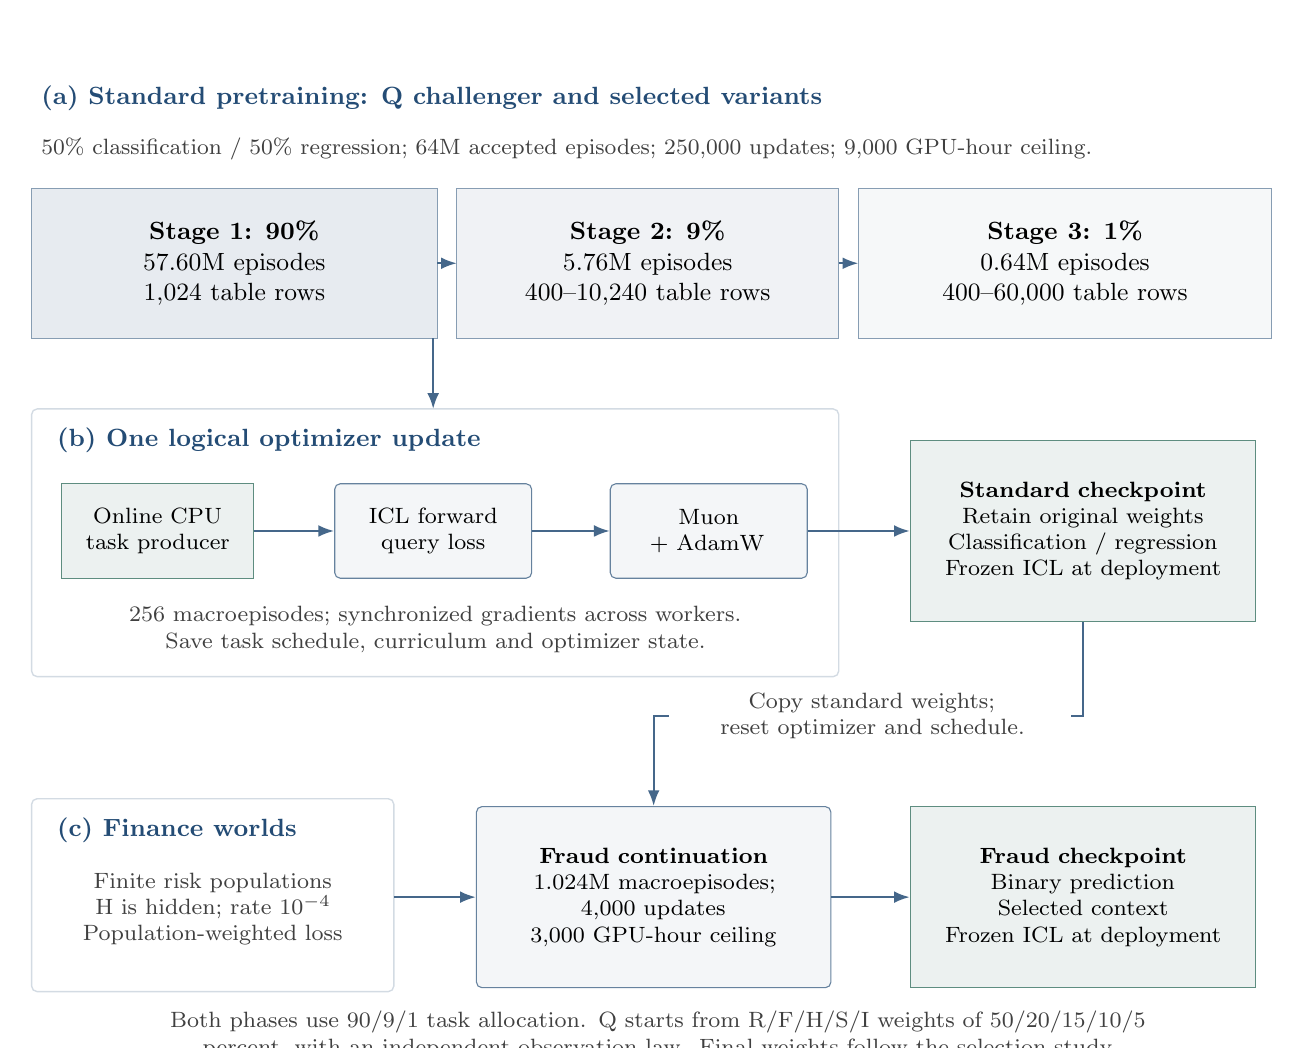
\begin{tikzpicture}[x=1cm,y=1cm,
  font=\small,
  panel/.style={draw=pfnblue!20,line width=.5pt,rounded corners=2pt,fill=white},
  title/.style={font=\small\bfseries,text=pfnblue,anchor=west},
  note/.style={font=\footnotesize,align=center,text=black!75},
  process/.style={font=\footnotesize,draw=pfnblue!70,fill=pfnblue!5,rounded corners=2pt,align=center,inner sep=5pt},
  support/.style={font=\footnotesize,draw=pfngreen!75,fill=pfngreen!9,align=center,inner sep=4pt},
  query/.style={font=\footnotesize,draw=pfnblue!70,fill=pfnblue!8,align=center,inner sep=4pt},
  hidden/.style={font=\footnotesize,draw=pfnamber!80,fill=pfnamber!8,align=center,inner sep=4pt,dashed},
  flow/.style={-{Latex[length=2mm]},draw=pfnblue!85,line width=.8pt},
  target/.style={-{Latex[length=2mm]},draw=pfnamber!90,line width=.8pt,dashed},
  reuse/.style={-{Latex[length=2mm]},draw=pfngreen!90,line width=.8pt,dashed}]

\path[use as bounding box] (0,.2) rectangle (16,-12.4);
\node[title] at (.05,-.2) {(a) Standard pretraining: Q challenger and selected variants};
\node[note,anchor=west,align=left] at (.05,-.85)
  {50\% classification / 50\% regression; 64M accepted episodes; 250,000 updates; 9,000 GPU-hour ceiling.};
\draw[draw=pfnblue!55,fill=pfnblue!11] (.05,-1.35) rectangle (5.2,-3.25);
\draw[draw=pfnblue!55,fill=pfnblue!7] (5.45,-1.35) rectangle (10.3,-3.25);
\draw[draw=pfnblue!55,fill=pfnblue!4] (10.55,-1.35) rectangle (15.8,-3.25);
\node[align=center] at (2.625,-2.3)
  {\textbf{Stage 1: 90\%}\\57.60M episodes\\1,024 table rows};
\node[align=center] at (7.875,-2.3)
  {\textbf{Stage 2: 9\%}\\5.76M episodes\\400--10,240 table rows};
\node[align=center] at (13.175,-2.3)
  {\textbf{Stage 3: 1\%}\\0.64M episodes\\400--60,000 table rows};
\draw[flow] (5.2,-2.3)--(5.45,-2.3);
\draw[flow] (10.3,-2.3)--(10.55,-2.3);
\draw[panel] (.05,-4.15) rectangle (10.3,-7.55);
\node[title] at (.25,-4.55) {(b) One logical optimizer update};
\node[support,text width=2.15cm,minimum height=12mm] (producer) at (1.65,-5.7)
  {Online CPU\\task producer};
\node[process,text width=2.15cm,minimum height=12mm] (model) at (5.15,-5.7)
  {ICL forward\\query loss};
\node[process,text width=2.15cm,minimum height=12mm] (optim) at (8.65,-5.7)
  {Muon\\+ AdamW};
\draw[flow] (producer)--(model);
\draw[flow] (model)--(optim);
\node[note,text width=9.4cm] at (5.15,-6.95)
  {256 macroepisodes; synchronized gradients across workers.\\Save task schedule, curriculum and optimizer state.};
\draw[flow] (5.15,-3.25)--(5.15,-4.15);
\node[support,text width=4.1cm,minimum height=23mm] (standard) at (13.4,-5.7)
  {\textbf{Standard checkpoint}\\Retain original weights\\Classification / regression\\Frozen ICL at deployment};
\draw[flow] (optim.east)--(standard.west);
\draw[panel] (.05,-9.1) rectangle (4.65,-11.55);
\node[title] at (.25,-9.5) {(c) Finance worlds};
\node[note,text width=4.05cm] at (2.35,-10.5)
  {Finite risk populations\\H is hidden; rate $10^{-4}$\\Population-weighted loss};
\node[process,text width=4.15cm,minimum height=23mm] (continuation) at (7.95,-10.35)
  {\textbf{Fraud continuation}\\1.024M macroepisodes; 4,000 updates\\3,000 GPU-hour ceiling};
\node[support,text width=4.1cm,minimum height=23mm] (specialist) at (13.4,-10.35)
  {\textbf{Fraud checkpoint}\\Binary prediction\\Selected context\\Frozen ICL at deployment};
\draw[flow] (4.65,-10.35)--(continuation.west);
\draw[flow] (continuation.east)--(specialist.west);
\draw[flow] (standard.south)--(13.4,-8.05)--(7.95,-8.05)--(continuation.north);
\node[note,fill=white,inner sep=3pt,text width=4.9cm] at (10.7,-8.05)
  {Copy standard weights;\\reset optimizer and schedule.};
\node[note,text width=15.4cm] at (8,-12.1)
  {Both phases use 90/9/1 task allocation. Q starts from R/F/H/S/I weights of 50/20/15/10/5 percent, with an independent observation law. Final weights follow the selection study.};

\end{tikzpicture}
\caption{Pretraining and synthetic fraud specialization for the implemented Q candidate and subsequent selected variants. Each run allocates 90/9/1\% of its accepted tasks to the three curriculum stages; stage boxes are not drawn in proportion to exposure. Task counts are planning targets constrained by the GPU-hour ceilings and measured throughput; the repository contains both shorter reference pilots and provisional full-volume Q configurations. Both resulting checkpoints use frozen-weight ICL at deployment. The final run uses the prior and architecture chosen by the controlled comparison.}
\label{fig:training-run}
\end{figure}

Both training phases use the same computational cycle:
\begin{enumerate}
\item A deterministic schedule specifies the task seeds and curriculum stage. The CPU producer prepares forthcoming tasks alongside model computation, and the trainer consumes them in the scheduled order.
\item The predictor receives support labels and query features, while the loss object holds query labels. Classification is scored by cross-entropy and ordinary regression by mean pinball loss. Binary-fraud losses retain their finite-population importance weights.
\item Route losses are reduced with the original macroepisode query denominator. Macroepisodes are then averaged over the global batch, gradients are synchronized across ranks, and the global gradient norm is clipped at ten.
\item Muon updates the registered hidden attention/FFN matrices, and AdamW updates the other parameters. Only a valid update advances the fixed warmup/cosine schedule. A change in weights requires model caches to be recomputed.
\item The trainer records consumed tasks, rejected generator attempts, aggregate row/cell counts, requested and observed class counts, update status and allocated time. The observed class count covers the support/query union, so these records are not full support-only coverage histograms. Checkpoints preserve the state required to reconstruct the deterministic schedule.
\end{enumerate}

Tasks are generated on demand from their seeds, so training does not require a stored copy of the complete bank. Bounded prefetch allows some CPU generation to overlap model computation, although its useful overlap and the resulting GPU utilization still require hardware measurements. Section~\ref{sec:volume} relates the complete update cost to a feasible training horizon; Section~\ref{sec:optimizer} specifies the optimizer equations and parameter groups.

\subsection{Typed data boundaries and deterministic replay}
\label{sec:training-contract}

Generation separates the statistical choices that define a problem from the observations presented to the learner. It draws the task and shape, samples hidden mechanisms, performs independent calibration where needed, simulates records and constructs the observed episode. Rendering determines the visible values and category identities. Preprocessing is then fitted on permitted support, and the adapter separates model inputs from query targets and simulator diagnostics. These responsibilities are expressed through the \texttt{Episode} interface described in Section~\ref{sec:code-map}.

The CPU reference requires a documented counter-based RNG or NumPy \texttt{SeedSequence}. Its streams are keyed by \texttt{(run\_seed}, \texttt{global\_episode\_id}, \texttt{recipe\_version}, \texttt{component\_id}, \texttt{attempt\_id)} through stable byte serialization and hashing. Python's process-randomized \texttt{hash()} is unsuitable for this purpose. Separate stream IDs identify profile, mechanism, calibration, support, query, observation and permutation draws, so a rendering change does not alter the underlying score or label-noise stream.

Reproducible recovery requires accepted IDs, retry counters, queue offsets and sampler state in the checkpoint. Model comparisons pair mechanism seeds, while training, calibration, synthetic validation and final audit use disjoint seed namespaces.

The minimal record below separates these roles explicitly. Arbitrary IDs express equality and carry no scalar measurement meaning:
\begin{lstlisting}
EpisodeSpec:
  recipe_version, episode_id, family, task_kind
  support_size, query_size, feature_budget, shape_bucket
  split_policy, class_vocabulary, active_modifiers
WorldParameters: mechanism graph, coefficients, latent effects, render rules
SafeInputs:
  support: features, categorical types, masks, observed_targets
  query: features, categorical types, masks
  metadata: declared task type and legal label vocabulary
LossOnly:
  query_targets, optional exact conditional label law
AuditOnly:
  latent states, true parameters, oracle predictions, rejection reasons
\end{lstlisting}
The task vocabulary and target definition precede scored outcomes and therefore cannot encode the number of classes realized in the query. The forward call excludes both \texttt{LossOnly} and \texttt{AuditOnly} from its \texttt{model.forward} argument. Debug fields likewise have no role in retrieval, cache keys, scaling or attention.

\subsection{Sampling, validity and retry semantics}

The authored-bank control samples P0/P1/P4 with probabilities 0.85/0.10/0.05, followed by mechanisms and modifiers conditional on the selected family. Its legal conditional probabilities balance binary, multiclass and regression tasks. Finance instead follows its separate finite-population sampler. Accepted task frequencies and the explicit loss normalization are recorded to distinguish these choices from their realized training exposure.

The selected shared head uses an ex-ante declared label vocabulary and permits classes to be absent from support. Legacy sampling that requires coverage is outside this default. Exceptions terminate the authored generator immediately, and the process producer preserves that behavior. Native R follows the released filter and retry semantics, with explicit counters and an abort bound.

Validity failures include invalid keys, nonfinite latent propagation, impossible shapes and simulator-budget violations. They do not include query imbalance or high query loss, and an entirely masked target cannot be replaced by zeros. The authored control accepts on validity alone, whereas native R retains the released predictability filter.

The optional queue adapter below would make up to eight attempts within the originally chosen family, using new streams for each attempt. Exhaustion would record a dropped request whose quota is replenished later. This adapter is a proposed extension, not the current training loop: it cannot replace a failing request with an easy linear task or conceal repeated failures.

Thus \texttt{validity\_only} acceptance in the authored control and the native teacher filter in R define different training laws. The optional adaptive policy in Section~\ref{sec:adaptive-training} changes future sampling weights using independent calibration worlds. It does not add an easy/medium/hard acceptance mixture to the base sampler.

\Needspace{7\baselineskip}
\begin{lstlisting}
for request_id in deterministic_request_stream:
    spec = sample_family_shape_task(request_id)
    for attempt in range(8):
        params = sample_parameters(spec, stream("mechanism", attempt))
        cal = independent_calibration(params, stream("calibration", attempt))
        freeze_mechanism_scales_and_task_thresholds(params, cal)
        world = simulate_world(params, stream("world", attempt))
        roles = choose_support_query_roles(spec, world)
        safe = compile_feature_views(world, roles, spec)
        loss = compile_targets_in_separate_object(world, roles, spec)
        if not validity_checks(safe, loss, params):
            log_invalid_request(spec, attempt)
            continue
        safe = support_only_preprocess(safe)
        yield safe, loss, separate_audit_record(spec, params, cal)
        break
    else:
        log_dropped_quota_request(spec)
\end{lstlisting}
The pseudocode describes an order of computation rather than the information boundary itself. A simulator may generate a complete joint table before extracting inputs. Feature selection, eligibility and task thresholds nevertheless remain independent of the realized scored query outcomes.

\subsection{Joint task mixture and finance-world reuse}
\label{sec:mixture}

The retained authored-bank sharing comparison allocates 80\% of emitted macroepisodes to the standard bank and 20\% to finance. The standard-family probabilities remain $.85/.10/.05$ for P0/P1/P4, while finance draws binary, multiclass and regression tasks with probabilities $.70/.10/.20$. Maintaining a one-third marginal allocation to each head then requires the following standard-component head probabilities:
\[
(.2416666667,\ .3916666667,\ .3666666667).
\]
Accounting for P4's binary/regression probabilities $.20/.80$ gives generic P0/P1 head probabilities $(.2438596491,.4122807018,.3438596491)$. This adjustment applies only to the joint experiment; the pure-standard control retains its original balanced marginal task distribution. The comparison reports raw profile frequencies alongside gradient and compute shares, since a 20\% macroepisode share implies neither 20\% of processed contexts nor 20\% of GPU-hours.

Profile membership is sampled for each emitted macroepisode. Sampling an 80/20 mixture of worlds and then reusing finance worlds four times would instead yield 50\% finance episodes. Each finance world, finite history and index is reused for four macroepisodes, with at most one use per logical optimizer batch. Model activations are recomputed at the current weights.

Each macroepisode draws 128 query IDs under the proposal in Section~\ref{sec:finance-objective}. Their features determine the routes, and every nonempty route group is evaluated. First-stage finance widths are $16,32,64,128$ with probabilities $.45/.25/.15/.15$; intermediate widths are $64,128,256,512$ with probabilities $.25/.35/.25/.15$; final widths are $128,256,512$ with probabilities $.25/.375/.375$. The stage cell cap applies to each routed forward using its actual support and query counts. Profiling sums computation across routes because a macroepisode can require more than one bounded forward.

\subsection{Likelihoods, preprocessing and logical-batch reduction}
\label{sec:training-loss}

Input and target transforms are fitted using only permitted support information, as specified in Sections~\ref{sec:codec} and~\ref{sec:heads}. The finance feature codec uses the selected reservoir from Section~\ref{sec:finance-context}. Under the inductive protocol, query features do not update those statistics. The masks in Section~\ref{sec:attention} keep support states independent of queries and each query independent of the others. This separation between model inputs, losses and hidden audit state continues through preprocessing and batching.

The original control scores standard classification with cross-entropy and ordinary regression with histogram/Lomax NLL. The selected candidate retains classification cross-entropy but replaces ordinary-regression NLL with the averaged 999-quantile pinball score. Realized finance loss uses the zero-atom likelihood in Section~\ref{sec:finance-head}.

A standard macroepisode averages its valid query losses, and the logical batch averages those macroepisode losses. Head multipliers initially equal one. Finance reduction instead retains the original query denominator and the selected world multiplier defined below; route groups are computational subdivisions rather than independently averaged episodes.

The funded prior comparisons hold the authored compressed architecture, preprocessing, prediction heads and optimizer fixed. A reproduction of the complete open reference would use its own recipe and constitutes a different comparison. Per-head gradient norms and validation quality are monitored because proper likelihoods expressed in different units do not directly measure comparable difficulty. Optional exact conditional targets are restricted to loss estimation under the eligibility rules in Section~\ref{app:staticrecipe}; they leave the forward interface unchanged.

Packing and accumulation preserve episode isolation: altering query labels or another packed episode leaves the relevant forward prediction unchanged. Macroepisode losses are summed and divided by the global accepted macroepisode count. Averaging unequal microbatch means would change those task weights.

\subsection{Population-risk estimation for rare-event queries}
\label{sec:finance-objective}

Consider a fixed finite future population $Q$, with class counts $m_y$ and total size $n_Q$. The query proposal draws a class from $r_y$, uniformly over classes present in the population, and then a uniform finite ID within that class. Training permits replacement. When both binary classes are present, $r_0=r_1=1/2$; an absent class has zero proposal mass. Sampling occurs \emph{before} feature-based routing, giving the estimator
\begin{equation}
\widehat{\mathcal L}(H)=\frac{w(H)}{q}\sum_{i=1}^{q}
\frac{m_{y_i}/n_Q}{r_{y_i}}\,\ell\bigl(f_\theta(x_i;C_{c(x_i)},H),y_i\bigr)
\label{eq:finance-risk}
\end{equation}
which estimates $w(H)$ times the finite-population query risk without bias, conditional on the world and history. The proposal probability cancels within each class, leaving the corresponding population average. This is an ordinary weighted mean rather than a self-normalized ratio. Grouping computation by route preserves the original $q$ denominator for every group's loss sum; an equal average of route-group means would alter the objective. Finite-population class fractions remain in the loss object and never enter forward inputs or metadata.

Amount-regression queries are sampled uniformly with unit weights. Realized-loss queries use the same importance construction over zero and positive outcomes, scored by the hurdle likelihood. Finance training retains sampled hard labels because conditional-label supervision would require the outcome distribution given the observed features and masks. Conditioning only on the simulator's latent risk cell does not supply that distribution.

Every world in the selected specialist has $w(H)=1$. The retained entropy-normalization comparison assigns the following weight to finance classification and event-loss regression when a reference is available:
\[
w(H)=\frac{1}{\max\{h_2(\pi_{\rm ref}),10^{-4}\}},\qquad
h_2(p)=-p\log p-(1-p)\log(1-p).
\]
Here $\pi_{\rm ref}$ denotes the scalar Jeffreys-smoothed any-fraud reference for multiclass tasks; otherwise $w=1$. The denominator limits amplification to 10,000. Since the multiplier is determined by permitted learner information, the ideal conditional optimum of a proper loss is unchanged, although a finite network can allocate capacity differently. Normalizing by \emph{hidden true} world entropy would instead reweight posterior worlds and could change the probability target.

The proposed comparison holds compute fixed between normalized and unnormalized losses and records clipping frequency under the norm-10 limit. The normalization cap remains an optimization choice to be tuned. A balanced proposal exposes more positive queries without creating independent positives in the finite history or removing every rare-event gradient problem. Focal loss and uncorrected class weighting remain comparison objectives rather than the default for estimating probabilities.

Selection also determines whether postprocessing is appropriate. For a classifier estimating the selected-example posterior $r(x)$, known retention probabilities $a_y(x)>0$ imply the following Bayes correction:
\begin{equation}
\operatorname{logit}p_{\rm pop}(x)=\operatorname{logit}r(x)+\log\frac{a_0(x)}{a_1(x)}.
\end{equation}
A scalar offset is valid under class-only selection, or an equivalent constant retention ratio, provided the prediction has the stated posterior interpretation. Local retrieval and selective label availability do not generally meet these conditions \cite{localcasecontrol}. The ICL objective already predicts population queries conditional on enriched support, so a second case-control correction would usually be inappropriate.

The three-state diagnostic recovered the population posterior to floating-point precision using the feature-dependent ratio. A scalar class correction instead incurred maximum absolute error $.439$, while the weighted-query diagnostic matched finite-population BCE exactly. These results verify the identities without evaluating a trained fraud model.

The effect of world normalization depends on the current prediction. At $\pi_{\rm ref}=10^{-4}$, the entropy multiplier is $979.4$. Under the balanced binary proposal, weighted logit derivatives are $2(1-\pi)p$ for negatives and $2\pi(p-1)$ for positives. For calibrated predictions $p=\pi$, scaling by $979.4$ gives approximately $+0.196$ and $-0.196$; for $p=0.5$, the negative derivative becomes approximately $979.3$. Thus the multiplier by itself does not establish instability, and initializing from a valid reference logit matters.

Normalization nevertheless changes how complete-reference and incomplete-adjudication worlds compete for capacity and contribute to global clipping. The comparison will record pre-clipping gradient norms and cosine similarities by standard/finance task, head, reference availability and positive count. Both the normalized and unit-multiplier arms retain the importance ratio. These measurements precede the choice between Muon and AdamW because gradient allocation interacts with optimization.

The initialization probe in \path{research/probes/finance_gradient_probe.py} checks actual autograd derivatives without optimizer updates. Its seeds, configurations, paired inputs, source hashes and all cases are retained in \path{research/results/finance_gradient_probe.json}. It measures neither a learning curve nor production fraud performance.

\subsection{Gradient scale and fraud specialization}
\label{sec:specialist}

At $p=\pi=10^{-4}$, each balanced-proposal weighted binary logit derivative has magnitude $2\pi(1-\pi)\simeq2\cdot10^{-4}$. Ordinary balanced binary CE at $p=.5$ has magnitude $.5$, which is 2,500 times larger before profile mixing. Gradients from these tasks are summed at shared parameters before AdamW or Muon acts. Consequently, the fraction of finance worlds in the schedule alone does not determine their allocation of parameter updates.

The fixed-initialization tiny-model probe illustrates this difference. A finance world with a complete historical reference gave a trunk gradient norm of $7.82\cdot10^{-6}$ under unit weighting, compared with $.00954$ for a P1 binary task. Without the historical reference, the mean predicted event probability was about $.496$ and the gradient norm was $.105$. No optimizer steps were taken; the larger norm reflects the initial base-rate error rather than measured learning. These results motivate an explicit allocation experiment. More query samples reduce sampling noise, whereas discarding their importance weights changes the target posterior.

A separate fraud continuation isolates finance optimization from standard-task gradients while retaining the standard checkpoint. The specialist preserves the architecture and uses binary risk-partition worlds, hidden H and unit world normalization, with unchanged query importance weights. Its peak learning rates are tenfold lower: $8\cdot10^{-5}$ for Muon and $3\cdot10^{-5}$ for AdamW. Unit and entropy normalization remain a controlled comparison.

The \texttt{--initialize-from} command copies model weights into a separately accounted run, initializes a fresh optimizer and schedule, and records the parent checkpoint hash. Exact recovery of an existing run instead uses \texttt{--resume}.

\subsection{Muon and AdamW: partition, numerics and schedule}
\label{sec:optimizer}

The optimizer partition follows the \href{https://github.com/KellerJordan/Muon}{original Muon implementation}, which pairs hidden-matrix updates with a conventional optimizer for embeddings and outputs. Shape-scaled updates and decoupled decay are motivated by \href{https://arxiv.org/abs/2502.16982}{Moonlight}. The \href{https://docs.pytorch.org/docs/2.14/generated/torch.optim.Muon.html}{PyTorch Muon specification} distinguishes the original scaling from \texttt{match\_rms\_adamw}; learning rates have meaning only together with the chosen convention. These sources inform the configuration but do not identify an optimum for this architecture or its AMD implementation.

Within each MAB, Muon acts on the four attention projections and three SwiGLU matrices. Q, K and V remain separate for orthogonalization even if the forward kernel is fused. AdamW handles the input, label and output projections, embeddings, inducing and summary tokens, norms, frequencies and scalar temperatures.

The chosen Muon configuration has peak base learning rate $8\cdot10^{-4}$, momentum 0.95, Nesterov momentum, five Newton--Schulz iterations with coefficients $(3.4445,-4.775,2.0315)$, epsilon $10^{-7}$ and zero weight decay; the original control uses decay 0.01. After gradients are synchronized, the momentum and update matrices are $B\leftarrow0.95B+g$ and $G\leftarrow g+0.95B$.

When rows exceed columns, $G$ is transposed. The matrix is normalized by its Frobenius norm plus epsilon, after which $A=XX^\top$ and $X\leftarrow aX+(bA+cA^2)X$ are evaluated five times before transposing back if necessary. Decay uses the base learning rate, while the matrix update is scaled by $0.2\eta\sqrt{\max(m,n)}$. Orthogonalization initially runs in FP32; a BF16 implementation would be a separately validated speed optimization.

AdamW uses peak learning rate $3\cdot10^{-4}$, betas $(0.9,0.95)$, epsilon $10^{-8}$ and ordinary bias correction. Projection and head matrices have weight decay 0.01 in the control and zero in the candidate. Embeddings, norms, frequencies and scalars have zero decay. Both optimizers receive synchronized gradients after global norm clipping at 10. Matrix products use BF16, with FP32 master weights, optimizer states, reductions, losses, softmax and normalization accumulators.

The trainer replicates model and optimizer state and averages gradients after the complete logical batch. It first synchronizes parameter-activity flags. A locally inactive branch contributes zero when its parameter is active elsewhere, whereas a globally unused parameter receives neither an optimizer-state update nor decay. Muon then orthogonalizes each complete original matrix. Orthogonalizing arbitrary tensor-sharding slices would define a different optimizer.

Memory constraints may change local microbatch size and gradient accumulation, but the logical batch remains 256 macroepisodes with the finance weights and original route denominators specified above. Learning rates warm up linearly over the first $\lceil0.02T\rceil$ valid optimizer updates and then follow a cosine decay to 10\% of peak at update $T$.

The horizon $T$ is derived once from the declared run budget and measured stage-specific update costs, and is fixed with the curriculum boundaries in the manifest. Calibration and pilot costs belong within the 50,000 GPU-hour project ceiling. A nonfinite gradient skips the entire update and its schedule increment; three consecutive skips abort with diagnostics. EMA is initially disabled. The earlier AdamW comparison specifies peak rates $10^{-4},3\cdot10^{-4},8\cdot10^{-4}$; it is deferred under the current selection allocation. Reproduction arms, if separately funded, retain each reference system's published recipe.

\subsection{Shape and class curriculum}
\label{sec:curriculum}

One warmup/cosine schedule covers each \emph{declared run horizon} in Section~\ref{sec:optimizer}. For the selected candidate, the provisional 90/9/1 episode allocation in Section~\ref{sec:volume} sets the stage proportions. Measured costs may require a shorter run; its total $T$ and stage boundaries are fixed before launch. Neither the optimizer nor the learning-rate schedule restarts at a stage boundary. The charged GPU-hour cap still applies if the run costs more than estimated.

Compute-scaling comparisons require each intended endpoint to complete its own schedule or a matched terminal cooldown. An intermediate checkpoint from a much longer unfinished decay is not equivalent to such a run. Recovery therefore preserves model, optimizer, sampler and compute state at least hourly and at stage boundaries; restart tests verify episode IDs and loss masks.

The authored-bank comparison retains its original allocation of 60\% of training GPU-hours to first-stage shapes, 25\% to medium contexts and 15\% to long or wide cases. These are measured-cost shares rather than episode-family probabilities. Stage one samples the three 32--2,048 support buckets equally. Stage two places 40\% of episodes in the short buckets and 60\% in discrete log-uniform 2,049--8,192 support. Subject to memory feasibility and development gains, stage three uses 30\% short, 30\% medium, 25\% long (discrete log-uniform 8,193--32,768 support) and 15\% wide (discrete log-uniform 1,024--4,096 support). Query count remains capped at 128 unless a separate supervision-density experiment justifies a change.

Short-bucket replay retains the base feature-width distribution. Medium contexts draw widths $\{64,128,256,512\}$ with probabilities $.25/.35/.25/.15$. Long contexts use $\{128,256,512\}$ with probabilities $.25/.375/.375$. The wide bucket uses $\{512,1024\}$ with probabilities $.35/.65$. The wide bucket is separate because width 1,024 is impossible for $n_s\geq8193$ under the final-stage cell cap. Width selection follows the originally sampled bucket even when a class-dependent floor subsequently increases support size.

The three stage cell caps are $2^{19},2^{21},2^{23}$. After support size is drawn and its class-dependent floor applied, the width probabilities are renormalized over values satisfying $(n_s+n_q)p\leq C_{\rm cell}$. Width is then drawn from this conditional law. This changes the shape prior explicitly rather than deleting sampled columns. The realized width and context frequencies, together with padding, are recorded; any reduction in the caps is accompanied by the resulting distribution and frequencies.

A long stage that fails its quality or throughput criterion will yield its remaining allocation to the best confirmed shape mixture. The changed schedule is recorded before final evaluation. Family probabilities remain fixed within each stage of the first controlled run, while any curriculum modification is a separate ablation charged to the same budget.


\paragraph{Authored-control many-class curriculum.} The following class schedule belongs to the authored replacement; the selected reference-derived bank retains the native class-budget law and the previously specified envelope extensions. Stage one uses $3$--$10$ classes. Stage two draws $K$ uniformly within $[3,10]$, $[11,32]$ or $[33,128]$, selecting those intervals with probabilities $.70/.20/.10$. Stage three adds $[129,256]$ and assigns probabilities $.70/.20/.08/.02$.

The support floor $n_s\geq16K$ is followed by recomputation of the bounded query count. Since this floor changes the context distribution, the realized histogram is logged. From initialization, the shared head supports 256 classes and masks inactive logits according to the declared or support label vocabulary. Evaluation tasks beyond that limit are reported as unsupported rather than omitted. A dynamic class head would require a separate architecture extension and is not implemented in this recipe.

\subsection{Optional consistency and masked-conditional objectives}
\label{sec:auxiliary-training}

The selected candidate uses supervised task scores alone. The proposed consistency comparison below applies to the histogram control. It adds a second view to 25\% of episodes by permuting features before grouping, reseeding category codes and drawing a new injection of the declared labels into 256 output slots. Predictions are aligned by semantic class, and the two supervised losses are averaged. The consistency coefficient rises from zero at $0.2T$ to 0.05 at $0.4T$ and then remains fixed.

Classification consistency uses symmetric stop-gradient KL. Regression uses the corresponding KL over the 130 bin masses plus 0.1 times the mean squared difference between the two log tail scales, with a shared target transform. This is a consistency regularizer rather than the KL between complete continuous densities. Deleting an informative feature is not treated as a prediction-preserving transformation. InfoNCE remains disabled because different rows or classes are not necessarily valid negatives across different synthetic mechanisms.

A separate masked-conditional experiment would add an auxiliary task to 10\% of episodes with weight 0.1. An observed feature is chosen uniformly among those eligible from support availability, removed from both feature tensors and used as the auxiliary target. The original $y$ is discarded for this task, and preprocessing is refitted after removal.

Categorical retargeting requires an independently declared complete vocabulary of at most 256 values. A support-only vocabulary cannot guarantee a legal auxiliary query target, and query values cannot determine eligibility or skipping. An ineligible auxiliary copy is skipped while its original episode is retained. This objective remains disabled unless a comparison at matched compute demonstrates a benefit.

\subsection{Optional adaptive prior sampling}
\label{sec:adaptive-training}

Family weights remain fixed in the initial run. The optional adaptive sampler would assess each active subfamily every 2\% of the run budget using 256 independent candidate worlds. Each calibration episode uses the sampled support size, including the class-size constraint, and $n_q=\min(256,\max(16,\lfloor n_s/4\rfloor))$. A fixed portfolio of constant, linear/logistic, shallow-tree and nearest-neighbor predictors receives the same feature interface as the model. The diagnostic score is classification cross-entropy or support-standardized regression MSE.

Normalized teacher opportunity is the current PFN checkpoint's calibration loss minus the best calibration teacher's loss, divided by the constant predictor's calibration loss floored at $10^{-3}$. Subfamily means are shrunk toward zero by $m/(m+256)$ and clipped to $[-1,1]$, after which the within-family weights are updated as follows:
\[
\widetilde w_j\propto w_j^{(0)}e^{0.5g_j},\qquad
w_j^{\rm new}=0.9w_j+0.1\widetilde w_j.
\]
The new weights are projected onto the probability simplex intersected with the box spanning one-quarter to four times each initial active weight. Euclidean projection finds the clipping offset by bisection. A 10\% stream from the original fixed distribution is retained, and the update policy is frozen before a confirmatory run. This is a conservative proposed setting within the performance-driven mixture-adaptation approach studied by RTFM and DoReMi \cite{rtfm,doremi}, rather than a claim of novelty.

Because the teacher portfolio can itself be biased, adaptive weighting will be assessed by transfer to real, lineage-disjoint development tasks against the unchanged-weight control. Calibration worlds remain distinct from scored worlds: allowing a scored query's label to select its emitted episode would introduce an uncontrolled distribution change. The comparison will examine whole-task transfer and classification and regression separately, rather than optimize raw loss or predictor disagreement as ends in themselves.


\section{Model size and allocation of 50,000 GPU-hours}
\label{sec:compute}

The available allocation comprises eight nodes with eight MI355X GPUs per node, for 64 GPUs. Its 50,000 GPU-hour ceiling corresponds to 781.25 hours, or 32.552 days, of full-cluster use. That allowance covers research, failed runs, model selection, final training and evaluation together, rather than a single final checkpoint. AMD specifies 288\,GB HBM per device and an approximately 2.5 PFLOP/s dense BF16 matrix peak \cite{amd}. The memory is distributed across devices, and usable throughput depends on the workload.

\subsection{Model-size recommendation}

The size study starts from the 317M model with its reduced query cache and revised representations. Planned comparisons include the 315M compressed-row control, the released TabICLv2 backbone and a compact persistent-cell architecture. Relevant alternatives include EXAONE's approximately 21M CAST, which preserves feature detail through its depth, and LimiX-2's persistent feature/target design \cite{exaone,limix2}.

Comparing these systems at equal cost addresses performance within the project budget. Studying capacity more directly requires two sizes within a selected architecture family. Neither MoE nor a 1B model has an initial allocation.

Within an architecture family, the frontend and input/output semantics stay fixed while the ICL trunk varies in width and depth. Available width/layer pairs are $(512,12)$, $(768,12)$, $(1024,24)$, $(1280,24)$ and $(1536,32)$. Head count is width/64, and SwiGLU width is $64\lceil(11d/4)/64\rceil$. When the trunk width differs from 1,024, a projection maps the concatenated eight cell summaries to that width, with corresponding changes to trunk label, task and head dimensions.

Actual parameter counts define the resulting models: the pairs are screening labels rather than exact 50/100/315/500/1,000M sizes. They make later comparisons possible without committing the program to every size. Only two sizes are funded after architecture-family selection.

A small tabular model can learn a useful inference procedure from labeled context without storing every task-specific fact in its weights. Its computational cost nevertheless includes long contexts, repeated cells, ensembles, preprocessing and retrieval. This observation alone says little about where capacity saturates. Under its own recipe, LimiX-2 reports gains across 12.5M--406.2M, whereas particular depth increases in Mitra and TabICLv2 produced weaker or saturating gains \cite{limix2,mitra,tabicl2}. Which behavior applies depends jointly on architecture, generator, optimization and data scale. A curve varying size alone therefore does not identify a compute-optimal frontier.

\subsection{Training volume and computational units}

Chinchilla estimated the balance between language-model size and training tokens from many runs; its 70B/1.4T example gives 20 tokens per parameter \cite{chinchilla}. That empirical ratio is neither a theorem nor a universal constant across language-model objectives. PFNs need their own accounting because raw cells, compressed rows, label targets and independent synthetic worlds measure different aspects of training exposure.

The compute analysis requires the following quantities for every optimizer update:
\begin{enumerate}
\item accepted episodes and distinct world/mechanism IDs;
\item context rows, query rows and actually scored query targets;
\item raw observed cells, padded cells and per-stage feature-cell activations;
\item row tokens entering the ICL trunk, with an explicit definition;
\item measured end-to-end GPU-seconds, generation time and rejection cost;
\item estimated training FLOPs for the encoder, attention, FFNs, heads and rematerialization.
\end{enumerate}
Layerwise operations contribute to FLOP estimates; multiplying input-token counts by the number of layers would make them incomparable with ordinary language-model token counts. Repeated views, repeated epochs and multiple episodes from a single world are recorded separately.

The standard default draws an independent world for every episode. Finance reuses each finite world for four macroepisodes, as described in Section~\ref{sec:finance}, while separately counting routed forwards and repeated support. A throughput ablation could similarly reuse each calibrated world for four independent support/query draws, with at most one draw per logical batch and no reuse across training and validation namespaces. Equal reuse across worlds preserves the marginal prior but changes gradient correlation and the number of distinct mechanisms. It is therefore a named comparison rather than an unreported increase in table count.

For example, an episode containing 1,024 support rows, 128 queries and 64 features presents 1,152 row tokens, 73,728 raw cells and 128 supervised targets. These counts do not convert mechanically into independent examples. Independent 4,096-row calibration also consumes generation time even though its draws are not model-training tokens, so its cost belongs in sampler profiling.


\subsection{Volume accounting for the executable reference pilot}
\label{sec:volume}

The reference-pilot volume plan specifies \textbf{64,000,000 accepted standard tasks}, followed by \textbf{1,024,000 finance macroepisodes} for the separate specialist. Each task is a support/query problem, rather than one row or cell. These are explicit planning targets, not an optimum inferred from a scaling law, and the respective 9,000 and 3,000 GPU-hour ceilings remain binding.

Deterministic seeds and ordered prefetch generate tasks when needed; the full bank need not be materialized in advance. Validation uses separate fixed namespaces whose worlds are never recycled into training.

With global batch 256, the standard target requires 250,000 updates. Stages one, two and three receive 90/9/1\% of accepted tasks. This allocation of episodes differs from the authored control's 60/25/15 allocation of GPU-hours. The selected curriculum follows the native shapes in Section~\ref{app:staticrecipe}, together with the declared envelope extension in later stages.

\begin{table}[ht]
\centering\small
\begin{tabular}{@{}rrrrr@{}}
\toprule Stage & Updates & Accepted tasks & Expected R & Expected P1\\
\midrule
1 & 225,000 & 57,600,000 & 54,909,091 & 2,690,909\\
2 & 22,500 & 5,760,000 & 5,488,596 & 271,404\\
3 & 2,500 & 640,000 & 610,801 & 29,199\\
\midrule Total & 250,000 & 64,000,000 & 61,008,488 & 2,991,512\\
\bottomrule
\end{tabular}
\caption{Standard exposure targets. Source expectations account for requested-width eligibility and are rounded to whole tasks; they are not fixed quotas.}
\end{table}

Eligibility determines the realized source mixture. If $E_s$ requested-width slots in stage $s$ have at least eight features, the exact conditional expectation of P1 exposure is $0.05\sum_s E_s$ and R receives the remainder. The five-percent branch would select 3.2 million P1 slots before eligibility. Integrating the rounded-uniform width laws and long-row caps instead gives expected accepted exposures of about 2.992 million P1 and 61.008 million R tasks. With feature ceiling $F_{\max}$, eligibility has probability $P(F\geq8)=(F_{\max}-7.5)/(F_{\max}-1)$; stage three averages this over its log-uniform row law and width caps.

The expected counts assume the declared envelopes, no diagnostic shape overrides, and no failed, skipped or replayed updates. Actual finite runs need not meet those counts exactly, and the expectations are not hard bounds. P4 contributes zero reference-pilot tasks and remains an unfunded count/amount control in the current allocation. R's eight function types are components inside graphs, not eight separate table families. Dividing R's task allocation equally among MLPs, trees, products and the other node functions would therefore define a different prior. We retain the pinned graph and function-sampling laws and audit the properties they produce.

Classification and regression are equiprobable package draws, each accounting for 32 million tasks in expectation. The classification budget follows the native integer law, modified on envelope-extension slots, so binary and multiclass tasks are not equiprobable. Under the proposed envelopes, expected exposures are approximately 3.503 million binary, 28.497 million multiclass and 32 million regression tasks. The number of observed classes can still collapse during native generation.

The 20\% envelope extension produces 1,152,000 stage-two slots and 128,000 stage-three slots in expectation. These are subsets of the R/P1 draws, not additional episodes. Accounting distinguishes requested class budgets, observed classes, requested and accepted feature widths, eligibility and every rejection reason.

Finance requires 4,000 updates, allocated as 3,600/360/40 across the stages. The resulting macroepisode counts are 921,600/92,160/10,240. At four uses per finite world, these correspond to 230,400/23,040/2,560 worlds, or 256,000 in total, provided that attempts are neither skipped nor replayed and reuse groups do not cross stage boundaries.

Each use draws 128 query targets, yielding 131,072,000 nominal query uses. Repeated positive IDs are repeated observations of finite outcomes rather than independent fraud evidence, and route forwards do not add macroepisodes. Likewise, representing a few-million-row population lazily does not place that entire population in a transformer context.

On 64 GPUs, the 9,000 GPU-hour standard allowance provides 140.625 wall hours, while 3,000 finance GPU-hours provide 46.875. Before setup and checkpoint reserves, reaching the targets would require aggregate rates of 126.420 standard tasks/s and 6.068 finance macroepisodes/s. At batch 256, the corresponding maximum weighted mean update times are 2.025 and 42.1875 seconds.

For measured stage times $t_s$, the relevant mean is $0.90t_1+0.09t_2+0.01t_3$. It includes generation, all routed computation and synchronization. These rates specify the throughput required by the plan; they do not predict MI355X performance.

The planner \path{scripts/plan_prior_volume.py} stores the unmeasured targets in \path{research/results/prior_volume_plan.json}. Once supplied with a timing JSON, it computes their cost and the largest smaller horizon within each phase ceiling after reserved overhead. Standard horizons are rounded to 100-update blocks; finance horizons use 400-update blocks, preserving both 90/9/1 stage proportions and four-use world boundaries.

The chosen horizon and cosine schedule are fixed together, since interrupting a longer schedule at the budget limit is not equivalent to completing a shorter planned run. Until these timings exist, the candidate configurations remain capped pilots. The measurement schema and full arithmetic are provided in \path{docs/prior_volume.md}.

\begin{lstlisting}
python scripts/plan_prior_volume.py \
  --output runs/provisional_volume.json
python scripts/plan_prior_volume.py \
  --measurements runs/actual_stage_timings.json \
  --output runs/measured_volume.json
\end{lstlisting}

Published exposure counts provide context for the proposed scale. The released TabICLv2 scripts imply 35.2 million table presentations for each classifier or regressor, and Kumo reports approximately 35/71/137 million tables for its size variants \cite{tabicl-code,kumo}. These figures motivate an order of magnitude without establishing equal statistical independence, equal compute or an optimal volume for this model. Both measured learning curves and cost are needed to choose the stopping point.

\subsection{Compute model and profiling protocol}

A useful first approximation to forward-plus-backward cost for a full row transformer uses its dense projection parameter count $P$, depth $L$, width $d$ and number of processed rows $r$:
\begin{equation}
C_{\rm row}\approx6Pr+12Ld\,r^2.
\end{equation}
The attention products contribute the second term and can be substantial. The specified support-only key/value path permits an attention-pair count of $n_s^2+n_sn_q$ \emph{if the implementation actually avoids query key/value work}; a dense masked kernel may still compute larger padded products. The projection term $6Pr$ is also approximate for this asymmetric path.

Frontend ISABs, within-row feature attention, categorical gathers, output heads, optimizer steps and activation recomputation add further cost. Kernel profiling must therefore accompany the estimates with measured time.

For a dual-axis cell architecture, projection positions instead scale as roughly $rF$ per block and attention pairs as $rF^2+Fr^2$, with the architecture's own widths and masks. ICL-315 combines narrow cell processing with a wide row trunk. Multiplying its cell count by all 315M parameters would incorrectly assume that every parameter processes every cell; counting row tokens alone would omit the frontend.

Holding batch-times-rows fixed does not hold total computation fixed. Doubling row count and halving batch size approximately preserves projection work while doubling full row-attention work. Similarly, Flash-style attention reduces materialization and memory traffic without eliminating quadratic arithmetic. A curriculum with ``constant tokens per step'' can therefore have changing update costs.

Each representative shape mixture will be profiled after 200 warmup steps for at least 1,000 timed steps, or a ten-minute stable interval if that is longer. End-to-end timing includes generation, queues, backward computation, optimization, communication, calibration and periodic checkpoints. Runs on one GPU, one eight-GPU node and the intended multi-node topology will record allocated devices, completed accepted episodes and all counters.

A small, fast model may become communication-bound on 64 GPUs. Where that occurs, independent node-level research runs may make better use of the same project budget.

Measured allocated GPU-seconds per accepted episode, $c$, convert a budget of $H$ GPU-hours into
\begin{equation}
E=\left\lfloor\frac{3600H}{c}\right\rfloor.
\end{equation}
The following applies the 12,000 GPU-hour conditional final-training ceiling to the fixed example with 1,152 rows, 64 features and 128 queries. It is \textbf{only a sensitivity calculation}; none of its rates was measured on MI355X.
\begin{table}[ht]
\centering\small
\begin{tabular}{@{}rrrrr@{}}
\toprule
Assumed GPU-s/episode & Episodes & Row tokens & Query targets & Row tokens/300M params\\
\midrule
0.1 & 432M & 497.664B & 55.296B & 1,658.88\\
1 & 43.2M & 49.7664B & 5.5296B & 165.888\\
10 & 4.32M & 4.97664B & 0.55296B & 16.5888\\
\bottomrule
\end{tabular}
\caption{Illustrative throughput sensitivity, not throughput forecasts or recommended data budgets. Raw cell counts are 64 times row counts in this example.}
\end{table}
The sensitivity calculation shows why a prescribed token ratio cannot determine training volume without a measured stack. The calculator uses real counters to recompute the affordable volume, treating each candidate plan as an alternative allocation of the same budget rather than an additional allowance.

\subsection{Model size and training-volume experiments}

The size and volume study holds the prior, architecture family, optimizer convention, task/shape schedule and validation distribution fixed. Its 10,000 GPU-hour allocation first compares two sizes with two seeds and 500 hours per size/seed, totaling 2,000 hours. It then provides 3,000 hours for each of two distinct finalist packages and two 1,000-hour runs for cross-seed confirmation or unresolved rankings.

A package includes all classification and regression checkpoints; specialist costs also remain inside its allowance. Each endpoint completes its own schedule and intended short/medium/long curriculum, with measured stage feasibility required before launch. If architecture family remains unresolved, these runs compare two candidates rather than isolate a pure size curve.

The 3,000-hour comparisons remain fourfold smaller than the complete 12,000-hour final package. Their learning curves can guide selection and reallocation but cannot locate a precise compute optimum. Equal-FLOP diagnostics will supplement the primary equal-cost comparison, since preprocessing overhead and kernel efficiency vary across systems.

Each completed endpoint will be evaluated on independent synthetic validation and the fixed real development panel, with binary classification, multiclass classification and regression reported separately. An empirical learning-curve surface will be fitted only if the observed points support a stable trend. One possible diagnostic is
\begin{equation}
L(P,D)=L_\infty+A P^{-a}+B D^{-b},\quad A,B,a,b>0,
\end{equation}
where the data quantity $D$ has a fixed, documented definition and the shape mixture is unchanged. Under the idealized cost model $C=6PD$, an interior optimum satisfies
\begin{equation}
aA P^{-a}=bB D^{-b},\qquad
P^*=\left[\frac{aA}{bB}(C/6)^b\right]^{1/(a+b)}.
\end{equation}
Even this simplified optimum depends on fitted coefficients and exponents rather than a universal ratio of 20. The hybrid architecture has a different cost surface, requiring measured costs and numerical comparison of feasible allocations. A change in prior requires a new estimate of the synthetic-loss exponent, and likelihood alone does not establish predictive accuracy.

Uncertainty will be estimated by resampling independent dataset lineages and training seeds. Sensitivity analyses will omit individual sizes and data endpoints. Where extrapolated fits are unstable, selection will follow the measured performance--cost frontier, with intermediate continuation decisions permitting reallocation if learning curves cross.

Predictive performance is the primary selection criterion. A larger model can therefore be preferred if it improves the final task score within the overall budget, even when a smaller model costs less per prediction. Inference comparisons include single-pass prediction, fixed ICL ensembles and permitted context retrieval. All preserve frozen ICL weights; per-task gradient fine-tuning belongs to a separately named adaptation track rather than the primary product setting.

\subsection{Allocation of the project budget}
\label{sec:revised-budget}

\begin{table}[ht]
\centering\small
\begin{tabularx}{\linewidth}{@{}rYY@{}}
\toprule
GPU-hours & Purpose & Release condition\\
\midrule
5,000 & Systems, reference and evaluation acceptance & 2,500 reference inference/reproduction; 1,500 backend/profiling/recovery; 1,000 benchmark integration and cost forecasts.\\
15,000 & Mandatory controlled screens & Current breakdown in Section~\ref{sec:prior-selection}; it supersedes the earlier allocation preserved below.\\
10,000 & Size and longer finalist comparisons & Two sizes/two seeds at 500 hours; two 3,000-hour bridges; two 1,000-hour confirmations or ranking-resolution runs.\\
12,000 & Conditional final training & Total across all selected checkpoints, after bridge and confirmation gates. No automatic one-shared-model commitment.\\
5,000 & Locked evaluation & Cost the official roster and finance periods before launch; failures and inference ensembles count.\\
3,000 & Uncommitted reserve & Failed runs, unresolved rankings or a measured specialization need; assign explicitly before use.\\
\midrule
50,000 & Total ceiling & 32.552 full-cluster days at 64 allocated devices.\\
\bottomrule
\end{tabularx}
\end{table}

The current screen is specified in Section~\ref{sec:prior-selection}. The earlier allocation and its controls are retained in Appendix~\ref{app:earlier-allocation} for reproducibility; they do not add to the budget.

\paragraph{Conditions shared by the current and earlier allocations.}
A fresh final run fixes a new horizon. Continuation after a change in recipe or horizon is a separately accounted experiment, whereas exact-config recovery preserves the original run. Failed reproduction, negative transfer or unresolved bridge comparisons prevent automatic release of the final allocation. Any unassigned reserve remains unspent.

Model and optimizer state are replicated in the trainer, which explicitly synchronizes gradients after each logical batch. At the selected size, optimizer-state memory alone is unlikely to justify aggressive parameter sharding; long-context activations may be more demanding. Activation checkpointing will be used where measurements show a benefit. Muon's updates continue to act on complete matrices, since independently orthogonalizing sharded pieces changes the method.

Abundant HBM does not eliminate CPU-generation bottlenecks or limitations in ROCm attention support. Parameter count alone therefore determines neither a feasible batch size nor attainable throughput.

\subsection{Compute accounting tool}

\begin{lstlisting}
python research/probes/compute_plan.py --gpu-hours 50000 --gpus 64 \
  --output research/results/compute_plan_50000.json
python research/probes/compute_plan.py --measurements measured_profiles.csv \
  --output research/results/measured_compute_plan.json
python -m unittest discover -s tests -p test_compute_plan.py -v
\end{lstlisting}
The measurement CSV identifies a run through \texttt{config\_id}, \texttt{params} and \texttt{allocated\_gpus}, and records its duration in \texttt{wall\_seconds}. Exposure is recorded as \texttt{accepted\_episodes}, \texttt{rows}, \texttt{cells}, \texttt{query\_targets} and \texttt{core\_tokens}, with the token convention specified in \texttt{core\_token\_definition}. These counters are totals over the timed interval. Missing or zero measurement quantities are rejected, and the script does not infer an optimum from throughput alone.

Four local accounting tests passed, covering budget conservation, allocated-GPU time, quadratic attention cost and invalid-input rejection. GPU throughput and model learning curves remain unmeasured.


\section{Evaluation and promotion criteria}
\label{sec:evaluation}

Evaluation addresses two distinct claims: broad performance from frozen ICL on standard benchmarks, and useful rare-event prediction against tree models trained on the full eligible history. Generator diagnostics and mathematical identities establish the validity of the experiment but cannot establish either performance result. Latency will be measured on the same pipelines as predictive quality, including context construction and ensembles.

\subsection{Generator and model acceptance checks}

A substantial run requires reproducible generation and a correct prediction interface. The checks cover deterministic regeneration, finite numerical values and stable moments, nominal-category handling, support-only preprocessing, legal class masks, invariance to query-label mutation, packed-episode isolation and independence of query-batch predictions.

Regression tests examine density normalization and analytic means at bin boundaries, small and large tail scales, constant targets and extreme outliers. Muon is checked against a small unfused FP32 implementation, with exact parameter counts and optimizer partitions verified. These tests establish implementation correctness rather than predictive accuracy.

Distributional audits examine what generation actually produces after class floors and cell caps: support/query dimensions, unique world IDs, active dimension, tree occupancy, categorical concentration, missingness and coarsening, class entropy and prevalence, target tail mass, and accepted family/head frequencies. Stage-specific plots will be compared with development-table descriptors without access to locked test labels. Label noise, null signals and identical visible rows with different outcomes remain legitimate draws rather than automatic reasons for rejection.

Interpretation of the new bank first requires reproduction of the unchanged reference's reported evaluation behavior. Generator, architecture, optimizer and prediction head remain separate experimental factors, because architecture changes can affect preprocessing, throughput and loss scale. Lower training loss alone cannot identify a gain from the prior.

World seeds are paired where possible, with independent namespaces for evaluation worlds. Surviving combinations will be confirmed with at least three seeds across the funded screening and scaling runs. A single final long run retains additional final-run uncertainty, which will be reported.

\subsection{Standard benchmarks and inference tracks}

TabArena is the primary standardized endpoint. The published design uses three outer folds, repeated ten times for tables below 2,500 rows and three times otherwise. Its primary metrics are binary ROC-AUC, multiclass log loss and regression RMSE \cite{tabarena}. The current model protocol has eight inner folds and separates default, tuned and ensembled variants; a system entrant controls its pipeline within the assigned budget \cite{tabarena-code}.

The comparison fixes repository revision, dataset IDs, split hashes, model wrappers and checkpoint versions. TabArena-Lite serves integration and screening, while final evidence follows the full applicable protocol.

The frozen ICL candidate will be reported both as a single pass and with a fixed ensemble. The proposed screen uses 1, 4, 8 and 16 independent feature, category and class-encoding views. It averages class probabilities or predictive distributions before taking means. Validation chooses ensemble size, with latency and memory charged to that setting and the single-pass result retained.

Beyond the validated context limit, comparisons will include uniform or stratified support subsampling and feature-based or learned retrieval using only permitted labels and features. Validation selects retrieval policy and context length; scored query performance does not. A 32k training stage alone does not establish support for million-row contexts.

The reference roster includes TabPFN-3.5, TabICLv2, Kumo Tabular, Xiaomi, EXAONE, current TabFM, LimiX-2 and suitable TabDPT/Mitra variants, together with tuned CatBoost, LightGBM and AutoGluon in the appropriate model or system tracks. Official recommended defaults will be reproduced where possible. Each result will identify its inference mode and cost, distinguishing a bare frozen predictor from task adaptation or ensembling. Although predictive performance is the priority, comparison with a tuned system answers a different question from frozen ICL at equal budget.

TALENT, BCCO and CTR23 broaden the task coverage, while ScoringBench evaluates distributional regression. Applicable single-table BeyondArena slices provide additional robustness evidence. Each suite uses a fixed named task view: TALENT's 300-table base, paper-specific subsets and extensions are different collections. Its current threshold, HPO and support-cap policies also require pinning \cite{talent-code}. BCCO retains the released splits and an explicit aggregation rule \cite{bcco-code}. ScoringBench requires matched distribution adapters and reported coverage for each metric \cite{scoringbench-code}; improvement in CRPS need not imply improvement in RMSE.

Development, confirmation and locked evaluation are separated by dataset and source lineage, with related OpenML exports and targets deduplicated across suites. A benchmark repeatedly consulted to modify the prior becomes development evidence even when pretraining itself uses only synthetic data.

Coverage reports include failures, difficult classes, wide tables, memory limits and timeouts rather than silently excluding them. An unavailable competitor score remains unavailable; another model's score cannot replace it as a measured result.

\subsection{Finance evaluation against full-history trees}

The principal finance baselines are task-trained XGBoost, LightGBM and CatBoost with the full eligible history, identical point-in-time features and the same label cutoffs. Restricting those models to the ICL context would test a narrower claim. Native missing-value handling and point-in-time 7/30-day aggregates are included wherever every method has access to those features. Calibration and threshold selection receive an explicit budget. A tree/ICL blend is evaluated as a separate application system with its own fitting cost.

The initial tree screen will draw 32 seeded configurations per library on development periods, including each documented default, and confirm the best four at later development origins. Every method receives the same declared wall-clock tuning allowance, and unfinished trials are reported.

XGBoost uses histogram boosting with learning rate $\mathrm{LU}(.01,.2)$, equally likely maximum depths $3,5,7,9$, child weight $\mathrm{LU}(1,100)$, row and column subsampling $\mathrm U(.6,1)$, and L2 penalty $\mathrm{LU}(.1,100)$. LightGBM samples 15/31/63/127 leaves equally and a rounded minimum leaf count $\mathrm{LU}(20,2000)$, with the same learning-rate, subsampling and L2 ranges. Its documented bagging frequency is enabled whenever row subsampling is active. CatBoost samples depths 4/6/8/10 equally, uses the same learning-rate range and L2 penalty $\mathrm{LU}(1,100)$, and records categorical handling.

Each trial allows up to 5,000 boosting rounds, with 100-round early stopping on an adjudicated later validation period. Half of non-default trials omit class weights; the other half draw a positive multiplier log-uniformly from $1$ to $\min(1000,N_-/\max(M,1))$, or use the corresponding per-class rule for multiclass tasks. Regression and degenerate weighting intervals omit class weighting.

Weighting and probability calibration are distinct interventions. LightGBM's official documentation explicitly notes that imbalance weights can degrade probability estimates \cite{lightgbm-params,xgboost-params,catboost-params}. The proposed ranges are fixed before evaluation and do not claim an optimal HPO budget. CPU infrastructure and tree tuning are recorded as operational costs; they count as GPU-hours only when GPUs are allocated.

Finance evaluation uses rolling chronological origins and distinguishes event, arrival, prediction and label-availability times. Training sees only labels available at the cutoff. Later adjudicated development windows determine calibration and thresholds, and untouched future windows are scored at their natural prevalence.

Recurring customers are legitimate in the primary deployment test. Unseen-customer and unseen-campaign splits provide additional stress tests, while unresolved outcomes remain masked. Population precision cannot be established from selectively reviewed test data without representative audits or justified observation weights. With few positive events, the evaluation uses a small, predeclared threshold or calibrator family and reports uncertainty rather than relying on a flexible isotonic fit or a wide threshold search.

Finance metrics include average precision with an explicit convention; precision and recall at a daily review budget; recall at a predeclared precision requirement; false positives per million negatives; log loss and calibration; and amount-weighted captured loss. Transaction, account and campaign units are distinguished, with raw TP/FP/FN counts reported.

Thresholds are chosen using past validation only. Selecting a threshold to meet precision on the test set would not evaluate an operational decision. Uncertainty estimates respect shared time, entity and campaign dependence through blocked analysis, and reports retain periods with no positive events.

The relationship between prevalence, true-positive rate and false-positive rate is
\[
\mathrm{Precision}=\frac{\pi\,\mathrm{TPR}}{\pi\,\mathrm{TPR}+(1-\pi)\,\mathrm{FPR}}.
\]
For illustration, precision and recall targets of $.8$ at prevalence $10^{-4}$ require an FPR of approximately $2.0002\times10^{-5}$, or about 20 false positives per million negatives. With no observed false positives, the one-sided 95\% IID upper bound is $1-.05^{1/n_-}$. Reaching the illustrative operating point with that bound requires about 149,771 adjudicated negatives.

A natural million-row test set contains about 100 frauds in expectation. Detecting 80 of 100 independent frauds yields a two-sided exact 95\% recall interval of approximately $[.708,.873]$. These operating targets are examples rather than company requirements. Dependence can weaken both calculations, so evaluation needs an adequately large negative holdout and uncertainty estimates that respect campaign dependence.

The public Bank Account Fraud suite provides six synthetic datasets, each with one million rows, 30 features and eight months of data, including controlled imbalance and shifts \cite{baf}. It offers a useful development proxy. Its roughly percent-level prevalence and published TPR-at-5\%-FPR operating point, however, do not establish performance at one event in ten thousand. The official comparison and any additional base-rate stress test will therefore be reported separately. The operational claim still requires company data and sufficiently long adjudicated holdouts.

\subsection{GPU batch-latency measurements}
\label{sec:latency-evaluation}

Initial inference profiling will use one MI355X per replica. The 64-GPU cluster can run independent datasets or estimators without assuming that one table benefits from 64-way inference. Each measurement fixes the checkpoint, ROCm/PyTorch/kernel revisions, precision, preprocessing, support selector, ensemble count and output type.

End-to-end time includes the CPU codec and transfers, while model startup is reported separately. A cold context has an empty support cache with model weights already resident; it does not include downloading a fresh checkpoint.

The core profile grid uses $n_s\in\{512,2048,8192,32768\}$, $F\in\{16,64,256\}$ and $n_q\in\{128,1024,8192\}$, with binary, 10/100/256-class and regression heads. Additional stress cases use 65,536/131,072 support rows at $F=64$ and width $F=1024$ at $n_s=2048$. These exceed some training shapes and are tests rather than established capabilities. Real-table task timings accompany the controlled synthetic profiles, with failures, OOMs and every fallback recorded.

Each feasible shape receives five untimed warmups followed by twenty timed repetitions. Cold-context repetitions clear the support cache, and wall-clock intervals are bracketed by GPU synchronization. Diagnostic component times cover the codec, host/device transfer, support frontend and trunk, query frontend and trunk, and outputs. Overlapping execution means these components need not sum exactly.

Reported measures include median/p95 cold-context batch time, warm-cache batch time, rows per second and peak device memory. Ensemble measurements include every member and aggregation, naming both sequential and feasible parallel deployment settings. Warmups and failed trials remain charged to the profiling budget.

Query chunks are selected from $\{128,512,2048\}$ using the systems grid and available memory, without scored query labels. The execution chunk size is distinguished from the full query-batch size. Before timing comparisons, cached and uncached predictions, different chunk sizes and reordered queries are checked against FP32 reference tolerances. Observed BF16 error and changes to benchmark predictions are recorded. A faster kernel is eligible only after attention-mask equivalence is established.

Model selection will report quality against total batch time at each context size and feature width, with separate binary, multiclass and regression views. Full dense context is the quality reference wherever feasible. A nonsignificant difference is not evidence of equality.

Any acceptable noninferiority margin must be fixed before the relevant confirmation run. Without that product decision, lower latency alone cannot justify a candidate with worse point-estimated quality. The higher-quality variant remains available, and uncertainty is reported without claiming lossless compression.

\subsection{Statistical promotion gates and ablations}

The statistical analysis retains separate scorecards for binary classification, multiclass classification and regression, alongside the official overall aggregation. Comparisons are paired by independent source dataset; repeated folds are repeated measurements rather than new independent datasets. Reports include raw task metrics, benchmark ranks and uncertainty. Elo values from different competitor rosters are not combined into a universal score. Proper predictive losses and calibration complement the official primary metric rather than replace it.

The current prior-selection criterion is the paired proper-loss rule in Section~\ref{sec:prior-selection}. The earlier proposal targeted positive improvement on all three panels, at least 1\% on a predeclared loss scale and no more than 2\% deterioration on important slices. Those earlier thresholds are retained for provenance and are not additional promotion requirements for the new search.

The earlier ranking rule used $1-\mathrm{AUC}$ for binary classification; the new prior search uses log loss, while official benchmark reporting retains AUC. Other benchmark metrics are reported on their original scales. The analysis accounts for candidate selection and multiple comparisons. Improvement on two task types at the expense of the third is reported as a tradeoff and prompts reconsideration of the shared/specialist design.

The earlier comparison catalog is retained in \path{research/specs/ablation_plan.csv}; current funded comparisons are specified in \path{research/specs/prior_selection_v1.json}. The allocation is defined by Section~\ref{sec:revised-budget} and \path{research/specs/prior_bank_spec.json}. Confirmation fixes the comparator roster, dataset lineages, per-task normalization, practical margins, candidate set, inference policy, failure policy and scheduled analysis points in advance.

Repeated folds are first averaged within lineage. Paired lineage resampling then incorporates training-seed variation rather than treating every fold as independent. Multiple separately selected claims call for a familywise procedure such as Holm. A single claim requiring improvement on all three task types instead requires each of its three constituent tests to pass. Failure to reject a difference does not establish equivalence.

The local evaluator does not yet implement this full promotion runner or the official cross-suite protocol. Finance threshold assessment also requires more than a favorable point estimate: one positive alert without a false positive cannot establish high population precision.

The planned analysis freezes a small threshold family on validation and applies an uncertainty criterion that respects campaign and time dependence, followed by a single evaluation on untouched future data. Too few independent events leave the result unresolved; additional pretraining compute cannot repair that lack of evaluation evidence.

The optional 5\% real-data continuation study is restricted to source-lineage-disjoint development data, excludes locked benchmarks and preserves the frozen inference interface. It retains a synthetic-only checkpoint and discloses the additional supervision. Task-centric TabDPT results motivate this comparison \cite{tabdpt,taskcentric}, but neither justify contaminated evaluation nor allow its gains to be attributed entirely to procedural priors.

\subsection{Joint-model selection within the budget}

The selected sequence retains a protected standard checkpoint and trains a separate binary specialist. The finance module also supports a sharing comparison between pure-standard training and the 80/20 joint profile. A second comparison varies the full bounded selector against a context control while holding model, worlds, search coverage and optimization fixed.

Before the two expensive confirmatory arms are chosen, intermediate controls are assessed on the same development suite: rare prevalence alone, reservoir plus available positives, full selection and metadata, and structured masks and delay. The primary equal-compute comparison is complemented by an equal-world-count diagnostic to separate improved inference from additional data-processing effort.

A joint model can replace the selected sequence only if it preserves the standard binary, multiclass and regression criteria while improving the finance panel against tuned full-history baselines at declared operating points. Finance utility and benchmark rank remain separate outcomes so their average cannot conceal a failure.

The default package already retains the standard checkpoint and assigns 9,000 hours to its training and 3,000 to binary specialization. Replacing it with a successful sharing challenger requires a recorded selection decision. The complete final package remains within 12,000 hours; further continuation or recovery requires a named reassignment inside the project budget.


\section{Implementation and validation}
\label{sec:experiments}

The codebase provides the reference and authored control generators, the finance generator, dense ICL model and size grid, AdamW/Muon optimization, mixed-task training, checkpoint recovery, exact support caches, bounded finance inference and data/evaluation commands. The root \texttt{README.md} links to operating instructions in \path{docs/training.md} and \path{docs/data_and_evaluation.md}. The optional TabArena wrapper is described in \path{docs/tabarena.md}.

\subsection{Map from the recipe to the implementation}
\label{sec:code-map}

The modules under \path{src/tabular_foundation/} implement the challenger, reference pilot and finance workflow mapped in Table~\ref{tab:code-map}. The Q sampler and its independent observation law use the same episode contract and trainer. The conceptual records from Section~\ref{sec:training-contract} use \texttt{schema.Episode}, whose \texttt{model\_inputs()} method explicitly allowlists forward inputs. Additional priors and retrieval policies enter through this contract, preserving the exclusion of hidden simulator state from the predictor.

\begin{longtable}{@{}>{\raggedright\arraybackslash}p{.22\linewidth}>{\raggedright\arraybackslash}p{.29\linewidth}>{\raggedright\arraybackslash}p{.41\linewidth}@{}}
\caption{Scientific components and executable code. Module paths are relative to \texttt{src/tabular\_foundation/}.}\label{tab:code-map}\\
\toprule Component & Module & Responsibility\\\midrule\endfirsthead
\toprule Component & Module & Responsibility\\\midrule\endhead
Challenger bank & \path{challenger_prior.py} & Task/shape-first R/F/H/S/I dispatch, independent world streams, H fallback and fixed-source retry.\\
Response and observation & \path{selection_laws.py} & Calibrated class scores, regression noise, missingness and coarsening; diagnostics remain outside model inputs.\\
Reference bank & \path{reference_prior.py} & Verified upstream source, task/shape-first R/P1/P4 dispatch and generation audit.\\
Ordered producer & \path{producer.py} & Seeded CPU process generation, bounded ordered prefetch and finite-world cache.\\
Authored control & \path{static_prior.py} & \texttt{generate\_episode()}; frozen worlds, response laws, rendering and optional context controls.\\
Finance prior & \path{finance_prior.py} & \texttt{generate\_finance\_world()} and \texttt{sample\_macroepisode()}; finite identities, availability and future-query proposals.\\
Input boundary & \path{schema.py}, \path{codec.py} & Allowed forward fields, nominal types, support-fitted statistics, ranks and value payloads.\\
Context selection & \path{retrieval.py} & Reservoir codec, shared centers, streamed candidate search, deduplication and query routing.\\
Predictor and heads & \path{model.py}, \path{distributions.py} & Fourier encoding, dense frontend/trunk, masks, metadata, support caches and normalized outcome laws.\\
Optimization & \path{optim.py}, \path{train.py}, \path{runtime.py} & Muon/AdamW partition, macroepisode loss, synchronized gradients, horizon and recovery.\\
Inference & \path{inference.py}, \path{predict.py} & Frozen standard/finance predictors and prediction command.\\
Data and scoring & \path{data.py}, \path{metrics.py}, \path{evaluate.py} & Input validation, temporal contracts, task metrics and validation-selected thresholds.\\
Paired selection & \path{selection_evaluation.py} & Declared data panels, exact split coverage, paired losses and source-lineage uncertainty.\\
Comparisons & \path{profile.py}, \path{baselines.py}, \path{tabarena_adapter.py} & Timing, task-trained tree baselines and optional official-benchmark integration.\\
\bottomrule
\end{longtable}

The scientific specifications are stored in \path{research/specs/static_recipe_v3.json}, \path{research/specs/icl_architecture_v3.json}, \path{research/specs/finance_recipe_v3.json}, the latency/MoE specification \path{research/specs/latency_recipe_v3.json}, and the coordinating \path{research/specs/prior_bank_spec.json}. Executable modules reside in \path{src/tabular_foundation}, with run configurations in \texttt{configs} and instructions in \texttt{README.md}.

The coordinating specification's \texttt{prior\_selection} block identifies the current research recommendation. Its \texttt{main\_candidate} block and \path{docs/main_recipe.md} retain the executable pilot, while the older v3 specifications define authored controls. These research JSON files describe the scientific recipe rather than the trainer's configuration format. The standalone \LaTeX{} source contains the full recipe without external input files.

Implemented components comprise the five-way Q sampler, its response and observation laws, the compact persistent-cell model, paired standard-panel evaluation, the base and context-conditioned standard priors, eligible optional conditional classification targets, the finance generator and selector, and the dense architecture. Available options include the reference prior, hash-bit codec, selectable heads, logarithmic scaling, query KV grouping, risk-partition finance law and ordered process producer.

MoE, the general local/global context graph, feature feedback, auxiliary objectives, adaptive weighting and real-data continuation remain specifications for controlled experiments, not implemented trainer options. Experiment manifests and results must preserve this distinction between runnable methods and proposed comparisons.

\paragraph{Generation and recovery.} The producer in \path{producer.py} operates serially or through a configured pool of persistent spawned CPU processes per training rank. The new candidate configurations use two workers per rank and a four-task prefetch queue. It prefetches a bounded number of scheduled tasks and consumes their futures in predetermined order, preventing faster generators from changing the mixture. Bounded finance caches are keyed by world, stage, task and overrides. Raw data can be reused, whereas model states are recomputed. Worker exceptions propagate with their audit records.

Reference runs start with \texttt{PYTHONHASHSEED=0} because the unchanged upstream sampler depends on set iteration as well as numerical RNGs. CPU tests found identical trained parameters with serial and prefetched data supply. Generation and input-wait counters from rank zero are diagnostics rather than measurements of whole-cluster utilization.

Completed-attempt logs contain globally reduced source, eligibility, rejection and shape/class counts. Replayed attempts add consumed presentations. Failed partial batches are incomplete records and require both the generator exception audit and scheduler accounting.

\subsection{Running the selected recipe}
\label{sec:selection-running}

Set \texttt{standard\_prior=selection} to use the Q sampler. The \texttt{selection\_options} block supplies the five mechanism probabilities, five observation probabilities and context-conditioned complexity probability. These are independent experimental controls. Native task and shape sampling occurs before mechanism dispatch, so new sources do not require generating and discarding a graph task. R with identity observation reproduces the unchanged native output at a fixed seed. New sources preserve valid absent-class and no-signal realizations.

The starting configurations are \path{configs/selection_candidate_standard.json} and \path{configs/selection_candidate_fraud.json}. They contain the provisional 250,000- and 4,000-update horizons, global batch 256, 90/9/1 stage allocation, the candidate Muon/AdamW rates and zero weight decay. Their run ceilings are 9,000 and 3,000 GPU-hours. The fraud configuration requires a compatible standard checkpoint and initializes fresh optimizer state. These files make the initial hypothesis runnable; they do not declare it the selected winner or establish that the requested volume fits the hardware.

\path{scripts/materialize_prior_selection.py} freezes an actual phase into separate trainer configurations and a manifest. Phase P needs no earlier result. M, A, V and F require recorded decisions from the preceding comparisons; each decision contains the chosen mechanism and observation weights and a nonempty reference to its evidence. Architecture and continuation phases also require the chosen model and, where applicable, a real compatible parent checkpoint. The script checks those contracts but cannot decide whether a written scientific judgment is sound. It never creates a fictitious winner. Standard horizons must be multiples of 100 updates; finance phases use multiples of 400 to preserve both the stage proportions and four-use world groups. The common \texttt{--steps} option supports equal-episode diagnostics. For the primary equal-budget comparison, \texttt{--horizons} reads an exhaustive mapping from trial IDs to measured full-schedule lengths. Different per-task costs can therefore produce different episode counts at the same allocation. The manifest records equal package ceilings; actual consumption must also be reported.

\begin{lstlisting}
export PYTHONHASHSEED=0
python -m tabular_foundation.train \
  --config configs/smoke_selection.json \
  --output runs/selection_smoke
python scripts/materialize_prior_selection.py \
  --phase P --steps 1000 --allocated-gpus 64 \
  --output runs/phase-P
\end{lstlisting}

The smoke uses small diagnostic shapes and exercises generation, both task types, optimization and checkpoints. The 1,000-update phase command illustrates configuration generation; the research horizon must instead come from measured stage costs. The manifest lists exact config paths and output directories. \path{scripts/submit_training.py} turns a resolved config into a Slurm command, printing it by default and submitting only with \texttt{--submit}. It uses the active Python environment and limits scheduler wall time by the remaining run and project budgets. It requests CPU resources for the configured producers as well as GPU ranks. The same PyTorch code supports CUDA and ROCm builds; neither stack has been profiled here.

The materializer's \texttt{--evaluation-reserve-gpu-hours} option sets aside a declared number of hours per trial inside its package allowance and subtracts them from the training cap. The default is zero and is explicitly marked unreserved. Separate evaluation jobs do not update the ledger automatically. \path{scripts/record_allocation.py} reconciles their scheduler-billed cumulative consumption under the manifest's evaluation allocation ID, and can reconcile killed or resumed training under its original run ID. Repeating a total is idempotent; decreases are rejected and actual overspending remains recorded. Training and evaluation together must fit each package allowance.

The project ledger records consumed hours, not reservations for concurrent jobs. Full-cluster jobs should therefore be submitted serially, and scheduler-billed time must be reconciled after failures or kills. A budget stop before the declared horizon is recorded as such, rather than counted as a complete comparison. No full synthetic corpus is required in advance: deterministic online generation and bounded ordered prefetch supply the training tasks.

\paragraph{Real-data evaluation.}
The standard-panel command in \path{selection_evaluation.py} reads a declared development, confirmation or final panel. Each split names its dataset, source lineage, task, fold, legal class count and separate support/query files. Stable original-record IDs establish disjointness; missing IDs require an explicit verified split-provenance record. The runner rejects identical files, overlapping IDs, changed paired data and incomplete split coverage. A lineage declaration still requires a real provenance audit: software cannot infer that two renamed datasets are independent.

Evaluation uses the checkpoint's training seed and a separately recorded inference-view seed. It measures context setup and cached prediction separately, with 1, 4 or 8 paired views. Views run sequentially, so peak memory describes that policy rather than simultaneous retention of all view caches. The comparison averages folds and trained seeds within datasets, then uses the objective and source-lineage bootstrap in Section~\ref{sec:prior-selection}. Reduced diagnostic bootstrap or lineage counts cannot produce a confirmation-evidence flag. Failed tasks remain explicit and prevent silent subset comparisons. Hardware and software identities accompany timing measurements; the separate finance evaluator retains chronological label-availability and threshold-selection contracts.

The full panel schema, phase-decision schema, launch commands, recovery procedure and tests are documented in \path{docs/prior_selection.md}. The native-shape generator audit is executable through \path{scripts/audit_selection_priors.py}. It streams task summaries and failure records; a small-shape diagnostic is clearly identified as such. Support-cross-validated teacher learning curves remain a separate research analysis rather than an automated acceptance filter.

\subsection{From local checks to a cluster pilot}

Local validation begins with the environment described in the root \texttt{README.md} and \path{docs/training.md}. The test suite and tiny standard-selection and finance smoke configurations precede a GPU allocation. Their smaller models and simpler tables, together with increased prevalence in the finance smoke, make them pipeline checks rather than tests of the research hypothesis.

\begin{lstlisting}
python -m pytest -q
python -m tabular_foundation.train \
  --config configs/smoke_selection.json --output runs/selection_smoke
python -m tabular_foundation.train \
  --config configs/smoke_finance.json --output runs/finance_smoke
python research/probes/finance_design_probes.py \
  --output research/results/finance_design_probes.json
\end{lstlisting}



Prediction and data conversion are exercised through \path{docs/data_and_evaluation.md}, and the intended benchmark adapter is checked using \path{docs/tabarena.md}. Cluster work then pins the ROCm-compatible software stack and profiles one replica and one node, recording allocated GPU-seconds by stage. Those measurements determine the horizon and cell or microbatch limits before a distributed pilot. Selection of the final model and mixture follows reference reproduction and the planned comparisons.

Each training run writes to a new directory under \texttt{runs/}. An interrupted run resumes from its existing configuration and checkpoint, preserving sampler state and charged compute. The repository contains no competitive pretrained weights; disposable tiny-run artifacts are regenerated as needed. The operating guides maintain exact CLI arguments, schemas and cluster-launch procedures rather than repeating them throughout the report.

\subsection{Numerical and statistical checks}

Several details are necessary for the implemented objective to match its specification. Mixture weights apply to emitted macroepisodes: an 80/20 world split followed by fourfold finance reuse would yield 50\% finance episodes. Routed losses retain the original query denominator, and the realized-loss head represents zero with an explicit atom. Feature-dependent retrieval is trained against population queries because a scalar class-sampling correction cannot reverse that selection.

The implementation contract requires fully adjudicated reference cohorts, exposes their sizes to the model, and uses the same scalar reference smoothing in training and serving. Finance width follows the active curriculum stage, and distributed budget decisions are synchronized. Recovery retains compute charges incurred after the last saved checkpoint. Sparse multiclass tree baselines keep unseen-class examples in evaluation and report their coverage.

Tests cover parameter counts, generator replay and moments, query-label isolation, attention and cache invariances, density normalization and moments, optimizer partitions, checkpoint replay and distributed gradient reduction. Detailed findings and residual risks appear in \path{docs/audit.md}, with machine-readable results in \path{research/results/code_validation.json}.

\subsection{Design implications of the implementation audit}
\label{sec:independent-disposition}

The implementation audit found no direct query-label input leak and retained the support/query boundary, finite-population accounting, population-weighted loss, frozen-weight caches and explicit optimizer partition. Its counterexamples led to more precise affine target transforms, finer prediction heads, discrete identity inputs, logarithmic attention scaling and query KV sharing. They also motivated finance worlds that hide H from both the selector and predictor. The comparisons above will determine whether these corrections improve real-data accuracy.

The affine precision failure arose before histogram quantization. Targets $10^8$ and $10^8+1$, with center $10^8$ and scale $0.5$, were cast to FP32 before subtraction and both standardized to zero. The implementation now retains FP64 affine quantities through standardization and inversion to original units, while neural probability calculations remain in FP32. Serving preserves the recovered original-unit precision.

Tests exercise NLL, gradients, CDFs and quantiles, means, and the positive-truncated finance head. Finer bins alone could not have recovered a target difference already erased by the affine calculation.

These results motivate studying prior coverage and information preservation together. A broad generator offers little advantage if the predictor loses feature identity, small target differences or rare historical evidence. An expressive model likewise cannot infer structure it never encounters in training tasks. The proposed comparisons first isolate these mechanisms, then test their combination against reference foundation models and tree systems.

\subsection{Validation and limitations}

The earlier runtime audit passed \textbf{200 tests with no skips}, treating warnings as errors and including the two-process Gloo test. The suite covers source verification and replay, task and shape preservation, rejection accounting, categorical encoding, prediction heads, optimizer partitioning, support caches, checkpoint recovery and per-prior task counts. Environment details and results are retained in \path{research/results/code_validation.json}, with earlier records in \path{docs/audit.md}.

The earlier prior-selection specification follow-up added analytical identities, exposure accounting, dependency validation and invalid-input checks. Its focused run passed 45 tests with warnings treated as errors, without changing runtime generators or models. The subsequent implementation described here adds the challenger generators, common laws, persistent-cell comparator, phase configuration and paired evaluation. These are separate validation records rather than a reinterpretation of the earlier results.

The implementation follow-up passes all 354 tests with warnings treated as errors, including the opt-in distributed test using permitted loopback sockets. A real three-update training run also completed all three diagnostic stages through both serial execution and two local Gloo ranks. All 143 checkpoint tensors, losses and source counters matched exactly. A \texttt{persistent\_tiny} run completed the same training path. These tests use small CPU models and do not validate 64-GPU communication, accelerator kernels or the requested research volume. A separate generator diagnostic produced valid 512-feature, 256-class tasks for each of F, H, S and I, retaining absent support classes; its four worlds do not establish distributional coverage.

A separate two-worker generator audit accepted all 60 requested worlds at fixed 48-support, 24-query, 12-feature shapes with a four-class budget. It covered all five sources across the three stage settings without new-world numerical retries. This is an execution check of the audit command, not the proposed thousand-world native-shape study. The latter must retain eligibility fallbacks and count actual accepted sources. The records are in \path{research/results/selection_training_integration.json} and \path{research/results/selection_prior_smoke_audit.json}.

Integration tests trained tiny CPU models on standard and finance tasks. Over three updates, the two-process mixed-profile run differed from its serial counterpart by at most $6\times10^{-8}$ in any parameter. A separate three-update reference-prior run continued for four binary-specialist updates, exercising initialization and world reuse. That continuation represented a one-million-row lazy history at prevalence $10^{-4}$ and used a 256-candidate diagnostic selector.

A separate three-million-row simulation checked finite-population counts and row identities. The tests also exercised prediction, evaluation, profiling, CSV conversion and all three tree-library adapters. Their capped candidate selectors do not measure retrieval throughput over the full history.

Numerical probes examine learnability and conditional-gradient identities, rare-event weighting, cache arithmetic and MoE initialization. In small FP64 modules, dense-to-expert decomposition error was below $7\cdot10^{-16}$, widening error was zero, query-chunk error was below $1.4\cdot10^{-15}$, and gate-gradient finite-difference error was below $2.0\cdot10^{-11}$. Detailed results and source hashes are stored under \path{research/results}, with scripts in \path{research/probes}. These verify numerical identities rather than full-model training or accelerator kernels.

The 317M candidate has neither been pretrained nor evaluated on competitive benchmarks, and MI355X measurements are unavailable. Throughput risks remain in the CPU/FP64 codec and data transfers. The bounded task queue overlaps CPU generation with training, but the producer has no pinned-memory transfer stream or byte-bounded queue. The persistent-cell comparator and paired standard-panel evaluator are now implemented and checked locally. These checks do not measure accelerator throughput or real-data transfer.

The next experiments combine reproduction of the released reference with stage-specific training-cost measurements and fixed-budget comparisons of prior and architecture changes. Standard benchmarks and chronological finance evaluation remain separate endpoints throughout selection. The question is whether the proposed conditional structure survives context selection and representation well enough to improve prediction over reference foundation models and trees trained on the full history.

\appendix
\section{Earlier screening allocation and controls}
\label{app:earlier-allocation}

\paragraph{Earlier allocation retained for experiment provenance.}
The following table and its associated controls describe the previous screening plan. The selection program in Section~\ref{sec:prior-selection} replaces them, with phase budgets of 4,800, 1,800, 3,200, 2,800 and 2,400 GPU-hours. Running both programs would exceed the allocation. Their specifications remain available for an explicitly budgeted replacement experiment.

\begin{longtable}{@{}p{0.57\linewidth}p{0.23\linewidth}r@{}}
\toprule Earlier screen & Arithmetic & GPU-hours\\\midrule\endfirsthead
\toprule Earlier screen & Arithmetic & GPU-hours\\\midrule\endhead
Prior triage: R, R+P1, R+P4, authored replacement & $4\times2\times250$ & 2,000\\
Prior/backbone crossing: two priors; released, authored compressed, compact persistent-cell & $6\times2\times350$ & 4,200\\
Regression head: reference quantiles versus finer histogram & $2\times2\times150$ & 600\\
Category codec: scalar Fourier versus hash-bit candidate & $2\times2\times150$ & 600\\
Length scaling: current cap versus one chosen alternative & $2\times2\times150$ & 600\\
Shared versus classifier/regressor checkpoint packages & $2\times2\times200$ & 800\\
Muon/AdamW versus all-AdamW, including rate triage & $2\times2\times150$ & 600\\
Six finance controls & $6\times2\times200$ & 2,400\\
At most two complete combinations, two new seeds each & $2\times2\times800$ & 3,200\\
\midrule Total & & 15,000\\\bottomrule
\end{longtable}

Each row in the allocation table multiplies arms by seeds and \emph{total package} hours. Initial task-specific packages divide time equally between classification and regression under a fixed binary/multiclass policy; the allowance is shared across checkpoints rather than granted independently to each.

The prior/backbone comparison holds heads, supported class range, feature/target interface and optimizer convention fixed. Adapters for the reference generator and new heads are executable. Faithful training interfaces for the native backbone and compact CAST comparison still require implementation. Capacity differences across families remain part of the system comparison. The smaller head, codec and attention studies fund fresh paired controls; an arbitrary partial checkpoint from a longer cosine run cannot serve as a completed control at a matched horizon.

The second factorial prior will be a graft supported by triage, or the authored replacement if a recorded decision assigns it that role. If neither is supported, R is retained and the unused cells of the comparison matrix receive no automatic allocation. A combined P1/P4 graft also has no automatic funding.

The finer-histogram and reference-quantile comparison tests two viable readouts, with the coarse histogram retained as an inexpensive falsification baseline. The analytic stress test will select one length-scaling alternative for the paired GPU comparison. All short learning-rate trials belong within the 600-hour optimizer allowance, rather than an additional search budget.

The six historical finance comparisons hold the legacy class-conditional mechanism, population seeds, arrival process and observation law fixed except for the named intervention. The risk-partition candidate belongs to the complete-configuration confirmation and specialist runs. Isolating its mechanism would require a matched legacy comparison within those existing slots.

The controls are standard-only F0; joint 80/20 with the full selector and unit normalization F1; the same with entropy normalization F2; F2 with explicit H removed from both selector and model F3; F2 with a nondiscriminative generative H law F4; and reservoir-plus-positive selection F5 using the normalization fixed before that run. Every applicable arm retains the correct population importance weights. F5 requires a comparison with matching normalization to identify a selection effect.

For the pure-standard finance control, untrained finance-only adapters must be neutralized consistently to avoid introducing random metadata effects. Reference-present and reference-absent worlds are reported separately. The two funded final-confirmation slots include a challenger and its required full-selector control; they do not fund two new candidates plus an additional control.

Confirmation will train at most two complete configurations, including any required paired control, and evaluate finance alongside all three standard task types. It tests the combination because separately observed gains need not add. Short runs provide triage evidence rather than proof of final superiority. If 150--350 hours cannot cover the intended contexts at measured hardware speeds, the number of arms or their allocations must change before launch. An early-curriculum checkpoint in one arm is not comparable to a completed curriculum in another.

Generation, indexing, calibration, every routed prefill and failed allocations all contribute to cost. The reference prior, candidate heads and codecs, and grouped-query cache are runnable. The compact cell architecture and complete paired statistical runner still require implementation for their research comparisons.

MoE, general sparse attention, adaptive priors and auxiliary objectives remain deferred. Query-only KV grouping is implemented and will be assessed within the existing architecture/confirmation allocation, without additional funding. Final training shares a 12,000-hour ceiling between 9,000 standard hours and 3,000 fraud hours; these are combined allowances rather than separate entitlements for each checkpoint.


\clearpage
\begin{thebibliography}{99}
\small
\bibitem{tabpfn} Hollmann et al. \emph{TabPFN: A Transformer That Solves Small Tabular Classification Problems in a Second}. ICLR 2023. Supplied \texttt{tabpfn.pdf}. \url{https://arxiv.org/abs/2207.01848}.
\bibitem{tabpfn2} Hollmann et al. \emph{Accurate Predictions on Small Data with a Tabular Foundation Model}. Nature 637, 2025. Supplied \texttt{tabpfn2.pdf}. \url{https://doi.org/10.1038/s41586-024-08328-6}.
\bibitem{tabpfn25} Prior Labs Team. \emph{TabPFN-2.5: Advancing the State of the Art in Tabular Foundation Models}. 2025. Supplied v2, \texttt{tabpfn2.5.pdf}. \url{https://arxiv.org/abs/2511.08667}.
\bibitem{tabpfn3} Prior Labs Team. \emph{TabPFN-3: Technical Report}. 2026. Supplied \texttt{tabpfn3.pdf}. \url{https://arxiv.org/abs/2605.13986}.
\bibitem{tabpfn35} J\"ager et al. \emph{TabPFN-3.5: Technical Report}. September 2026. Supplied \texttt{tabpfn3.5.pdf}. \url{https://arxiv.org/abs/2609.17895}.
\bibitem{tabicl} Qu et al. \emph{TabICL: A Tabular Foundation Model for In-Context Learning on Large Data}. ICML 2025. Supplied \texttt{tabicl.pdf}. \url{https://github.com/soda-inria/tabicl}.
\bibitem{tabicl-code} Qu et al. \emph{TabICL official pretraining scripts and release notes}. Accessed October 3, 2026. \url{https://github.com/soda-inria/tabicl#pre-training}.
\bibitem{tabicl2} Qu et al. \emph{TabICLv2: A Better, Faster, Scalable, and Open Tabular Foundation Model}. 2026. Supplied v2, \texttt{tabicl2.pdf}. \url{https://arxiv.org/abs/2602.11139}.
\bibitem{tabfm} Kong et al. \emph{TabFM: A Zero-Shot Foundation Model for Tabular Data}. September 29, 2026. Supplied \texttt{tabfm.pdf}. \url{https://arxiv.org/abs/2609.37959}.
\bibitem{xiaomi} Xiaomi-TabLDM Team. \emph{Xiaomi-TabLDM: A Tabular Foundation Model Technical Report}. September 2026. Supplied v2, \texttt{xiaomi.pdf}. \url{https://arxiv.org/abs/2609.03880}.
\bibitem{exaone} Eo et al. \emph{EXAONE Tabular 1.0: Technical Report}. August 2026. Supplied \texttt{exaone.pdf}. \url{https://arxiv.org/abs/2608.25774}.
\bibitem{kumo} NVIDIA. \emph{NVIDIA Kumo Tabular Sets a New Accuracy-Efficiency Frontier for Tabular Prediction}. September 29, 2026. Supplied print \texttt{kumotabular.pdf}. \url{https://huggingface.co/blog/nvidia/kumo-tabular}.
\bibitem{mitra2} \emph{Mitra-v2 Technical Report}. September 2026. Secs.\ 2.2--2.4, Table\ 2, Appendix C. \url{https://arxiv.org/abs/2609.04540}.
\bibitem{oprior} Bouadi et al. \emph{Shaping the Prior: How Synthetic Task Distributions Determine Tabular Foundation Model Quality}. 2026. Sec.\ 3.1, Table\ 2. \url{https://arxiv.org/abs/2605.18971}.
\bibitem{mindgap} Davies et al. \emph{Mind the Gap? A Distributional Comparison of Real and Synthetic Priors for Tabular Foundation Models}. 2026. \url{https://arxiv.org/abs/2605.06343}.
\bibitem{prioreval} T\"urkmen et al. \emph{Towards Evaluating Data Priors for Tabular Foundation Models}. 2026. Secs.\ 3--4. \url{https://arxiv.org/abs/2606.29241}.
\bibitem{structuralcoverage} Zhao et al. \emph{From Synthetic Priors to Model Behavior: Structural Coverage in Tabular Foundation Models}. September 2026. \url{https://arxiv.org/abs/2609.06912}.
\bibitem{tabicl-weights} Qu et al. \emph{Official TabICL checkpoints}. Metadata inspected October 2, 2026; exact revisions in the model-scale audit. \url{https://huggingface.co/jingang/TabICL}.
\bibitem{kumo-weights} NVIDIA. \emph{Kumo Tabular official checkpoints}. Metadata inspected October 2, 2026. \url{https://huggingface.co/nvidia/Kumo-Tabular}.
\bibitem{tabfm11-weights} Google. \emph{TabFM 1.1.0 official PyTorch checkpoints}. Metadata inspected October 2, 2026. \url{https://huggingface.co/google/tabfm-1.1.0-pytorch}.
\bibitem{tabfm10-weights} Google. \emph{TabFM 1.0.0 official PyTorch checkpoints}. Metadata inspected October 2, 2026. \url{https://huggingface.co/google/tabfm-1.0.0-pytorch}.
\bibitem{limix2} LimiX Team. \emph{LimiX-2: A Contextual Mechanism Network Towards General Structured-Data Intelligence}. September 2026. \url{https://arxiv.org/abs/2609.17488}.
\bibitem{tabdpt-weights} Layer 6. \emph{TabDPT official checkpoints}. Version 1.3 metadata inspected October 2, 2026. \url{https://huggingface.co/Layer6/TabDPT}.
\bibitem{tabdpt} Ma et al. \emph{TabDPT: Scaling Tabular Foundation Models on Real Data}. NeurIPS 2025. \url{https://arxiv.org/abs/2410.18164}.
\bibitem{taskcentric} Shaheen et al. \emph{Understanding the Surprising Generalization Properties of Tabular Foundation Models}. August 2026. \url{https://arxiv.org/abs/2608.17957}.
\bibitem{sdd} Biswas and El Karoui. \emph{Distillation of Synthetic Data for Time Series Foundation Models}. September 2026, v2. \url{https://arxiv.org/abs/2609.09586v2}.
\bibitem{rtfm} Peroni et al. \emph{Robust Tabular Foundation Models}. 2025. \url{https://arxiv.org/abs/2512.03307}.
\bibitem{doremi} Xie et al. \emph{DoReMi: Optimizing Data Mixtures Speeds Up Language Model Pretraining}. NeurIPS 2023. \url{https://arxiv.org/abs/2305.10429}.
\bibitem{amd} AMD. \emph{AMD Instinct MI355X GPUs}. Official specifications, accessed October 2, 2026. \url{https://www.amd.com/en/products/accelerators/instinct/mi350/mi355x.html}.
\bibitem{mitra} Zhang et al. \emph{Mitra: Mixed Synthetic Priors for Enhancing Tabular Foundation Models}. NeurIPS 2025. \url{https://arxiv.org/abs/2510.21204}.
\bibitem{chinchilla} Hoffmann et al. \emph{Training Compute-Optimal Large Language Models}. NeurIPS 2022. \url{https://arxiv.org/abs/2203.15556}.
\bibitem{tabarena} Erickson et al. \emph{TabArena: A Living Benchmark for Machine Learning on Tabular Data}. NeurIPS 2025. \url{https://arxiv.org/abs/2506.16791}.
\bibitem{tabarena-code} AutoGluon team. \emph{TabArena repository: model/system protocols and TabArena-Lite}. Accessed October 2, 2026. \url{https://github.com/autogluon/tabarena}.
\bibitem{talent-code} LAMDA-Tabular. \emph{TALENT repository: datasets, evaluation, and tuning policies}. Accessed October 2, 2026. \url{https://github.com/LAMDA-Tabular/TALENT}.
\bibitem{bcco-code} LimiX team. \emph{LimiX repository and BCCO dataset releases}. Accessed October 2, 2026. \url{https://github.com/limix-ldm-ai/LimiX}.
\bibitem{scoringbench-code} Landsgesell et al. \emph{ScoringBench implementation and benchmark data}. Accessed October 2, 2026. \url{https://github.com/jonaslandsgesell/ScoringBench}.
\bibitem{flashattention} Dao et al. \emph{FlashAttention: Fast and Memory-Efficient Exact Attention with IO-Awareness}. NeurIPS 2022. \url{https://arxiv.org/abs/2205.14135}.
\bibitem{switch} Fedus et al. \emph{Switch Transformers: Scaling to Trillion Parameter Models with Simple and Efficient Sparsity}. JMLR 2022. \url{https://arxiv.org/abs/2101.03961}.
\bibitem{stmoe} Zoph et al. \emph{ST-MoE: Designing Stable and Transferable Sparse Expert Models}. 2022. \url{https://arxiv.org/abs/2202.08906}.
\bibitem{sparseupcycling} Komatsuzaki et al. \emph{Sparse Upcycling: Training Mixture-of-Experts from Dense Checkpoints}. ICLR 2023. \url{https://arxiv.org/abs/2212.05055}.
\bibitem{aiter} AMD/ROCm. \emph{AITER: AI Tensor Engine for ROCm}. Official operator repository, accessed October 2, 2026. \url{https://github.com/ROCm/aiter}.
\bibitem{settransformer} Lee et al. \emph{Set Transformer: A Framework for Attention-based Permutation-Invariant Neural Networks}. ICML 2019. \url{https://arxiv.org/abs/1810.00825}.
\bibitem{gqa} Ainslie et al. \emph{GQA: Training Generalized Multi-Query Transformer Models from Multi-Head Checkpoints}. EMNLP 2023. \url{https://arxiv.org/abs/2305.13245}.
\bibitem{baf} Jesus et al. \emph{Turning the Tables: Biased, Imbalanced, Dynamic Tabular Datasets for ML Evaluation}. NeurIPS 2022. \url{https://proceedings.neurips.cc/paper_files/paper/2022/file/d9696563856bd350e4e7ac5e5812f23c-Paper-Datasets_and_Benchmarks.pdf}.
\bibitem{fraud-realistic} Dal Pozzolo et al. \emph{Credit Card Fraud Detection: A Realistic Modeling and a Novel Learning Strategy}. IEEE TNNLS. Author manuscript. \url{https://dalpozz.github.io/static/pdf/TNNLS_2017.pdf}.
\bibitem{fraud-handbook} Le Borgne et al. \emph{Reproducible Machine Learning for Credit Card Fraud Detection: Practical Handbook}, validation strategies. \url{https://fraud-detection-handbook.github.io/fraud-detection-handbook/Chapter_5_ModelValidationAndSelection/ValidationStrategies.html}.
\bibitem{elkan-pu} Elkan and Noto. \emph{Learning Classifiers from Only Positive and Unlabeled Data}. KDD 2008. \url{https://cseweb.ucsd.edu/~elkan/posonly.pdf}.
\bibitem{localcasecontrol} Fithian and Hastie. \emph{Local Case-Control Sampling: Efficient Subsampling in Imbalanced Data Sets}. Annals of Statistics, 2014. \url{https://arxiv.org/abs/1306.3706}.
\bibitem{tabr} Gorishniy et al. \emph{TabR: Tabular Deep Learning Meets Nearest Neighbors}. ICLR 2024. \url{https://arxiv.org/abs/2307.14338}.
\bibitem{lightgbm-params} LightGBM authors. \emph{Official parameter reference}. \url{https://lightgbm.readthedocs.io/en/latest/Parameters.html}.
\bibitem{xgboost-params} XGBoost authors. \emph{Official parameter reference}. \url{https://xgboost.readthedocs.io/en/stable/parameter.html}.
\bibitem{catboost-params} CatBoost authors. \emph{Common training parameters}. \url{https://catboost.ai/docs/en/references/training-parameters/common}.
\bibitem{priorlabs-code} Prior Labs. \emph{TabPFN-3.5 implementation}, revision 15f5e6b, inspected October 3, 2026. \url{https://github.com/PriorLabs/TabPFN/blob/15f5e6b2b629b905879b9be907261416f20d0df5/src/tabpfn/architectures/tabpfn_v3_5.py}.
\bibitem{kumo-code} NVIDIA. \emph{Kumo Tabular ICL implementation}, revision b982fbf, inspected October 3, 2026. \url{https://github.com/NVIDIA/structured-data-models/blob/b982fbf4188ea8db17249fe81338723106100b63/sdm/models/kumo/tabular/icl.py}.
\bibitem{xiaomi-code} Xiaomi. \emph{Xiaomi-TabLDM public source}, revision c87efdd, inspected October 3, 2026. \url{https://github.com/xiaomi-research/xiaomi-tabldm/tree/c87efddedb244d1a21ac07b40b1453466329e5c5}.
\bibitem{mitra-code} AutoGluon. \emph{Mitra-v2 fine-tuning source}, revision b4701e8, inspected October 3, 2026. \url{https://huggingface.co/autogluon/mitra-finetune/tree/b4701e8148dc33b00ed15d7086ff59816957cde4}.
\bibitem{sparsealignment} Zhao et al. \emph{Architecture Alignment With Sparse Priors in Tabular Foundation Models}. September 2026. \url{https://arxiv.org/abs/2609.36883}.
\bibitem{memoryefficient} Luo et al. \emph{Memory Efficient Tabular Foundation Models}. July 2026. \url{https://arxiv.org/abs/2607.27546}.
\bibitem{lessconstrained} Park et al. \emph{Generating High-Diversity Synthetic Tabular Data via Less-Constrained Prior}. IJCAI 2026, pp. 4714--4722. \url{https://www.ijcai.org/proceedings/2026/525}.
\end{thebibliography}
\end{document}
